% Created 2023-09-03 dim. 21:37
% Intended LaTeX compiler: pdflatex
\documentclass[presentation]{beamer}
\usepackage[utf8]{inputenc}
\usepackage[T1]{fontenc}
\usetheme{default}
\author{Malik K. Koné}
\date{\today}
\title{Les suites}
\hypersetup{
 pdfauthor={Malik K. Koné},
 pdftitle={Les suites},
 pdfkeywords={},
 pdfsubject={},
 pdfcreator={Emacs 28.2 (Org mode 9.6.7)}, 
 pdflang={English}}
\begin{document}

\maketitle
\begin{frame}{Outline}
\tableofcontents
\end{frame}

{
  \usebackgroundtemplate{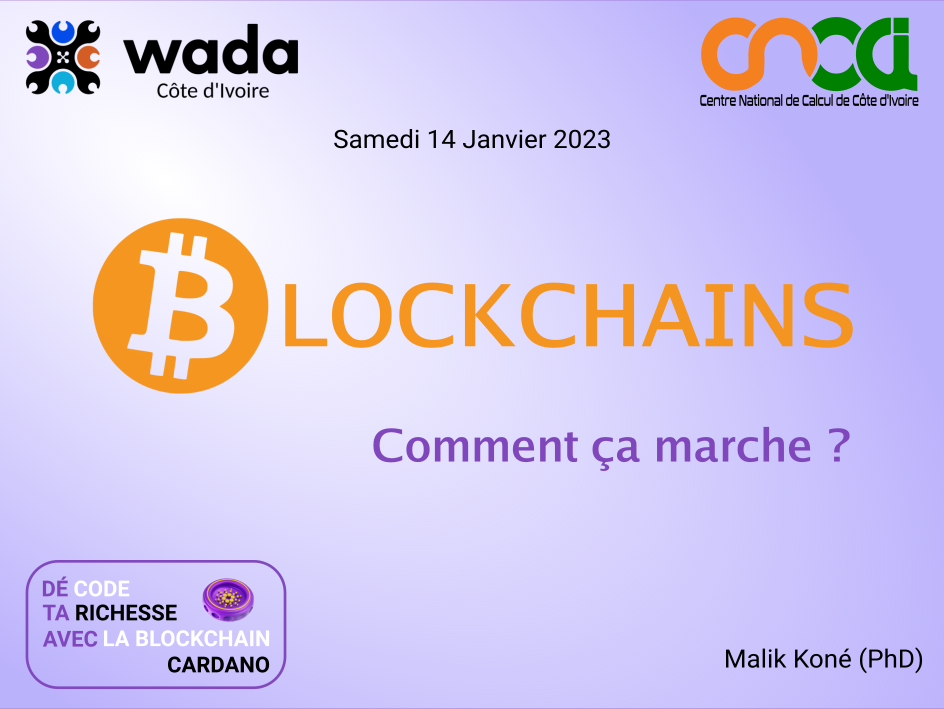
\includegraphics[height=\paperheight]{./page_de_garde_wadaci_j1a}}
  \frame[plain]{
  }
}

\section{Introduction}
\label{sec:org6f536e9}
\begin{frame}[label={sec:org1959b3f}]{Notions de départ}
\begin{block}{Notions de départ}
\begin{center}
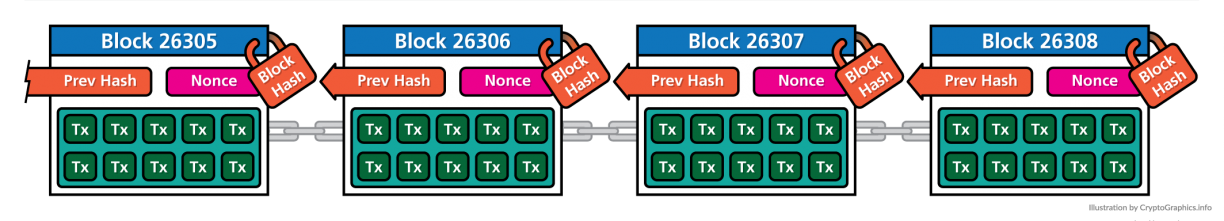
\includegraphics[width=\textwidth]{Pictures/cryptographics/anatomy-of-a-chain-1.png}
\end{center}

\begin{columns}
\begin{column}{0.54\columnwidth}
\begin{block}<1->{Blockchain}
\begin{itemize}
\item <2> Décentralisation
\item <2> Consensus
\item <2> Cryptographie
\item <2> Applications décentralisées (dApp)
\end{itemize}
\end{block}
\end{column}
\begin{column}{0.46\columnwidth}
\begin{block}<1->{Cryptoéconomie}
\begin{itemize}
\item <0>Tokens ou jetons
\item <0>Marchés financiers
\item <0>Porte-monnaie de crypto (\href{https://yoroi-wallet.com}{Yoroi-wallet})
\end{itemize}
\end{block}
\end{column}
\end{columns}
\end{block}
\end{frame}

\begin{frame}[label={sec:org7ff72af}]{Les types d'utilisateurs des Blockchain}
\begin{block}{Les rôles sur la blockchain}
\begin{columns}
\begin{column}{0.39\columnwidth}
\begin{block}{}
\begin{itemize}
\item <1>Les empereurs
\item <2>les élus
\item <3>les mineurs
\item <4>les utilisateurs
\end{itemize}
\end{block}
\end{column}
\begin{column}{0.6\columnwidth}
\begin{block}{}
\begin{figure}[ht]
  \centering
  \includegraphics<1>[width=\textwidth]{Pictures/user_empereur}
  \includegraphics<2>[width=\textwidth]{Pictures/user_elu}
  \includegraphics<3>[width=\textwidth]{Pictures/user_mineur2}    
  \includegraphics<4>[width=\textwidth]{Pictures/user_user2}
\end{figure}
\end{block}
\end{column}
\end{columns}
\end{block}
\end{frame}

\section{Bitcoin : Blockchain de 1\iere{} génération}
\label{sec:orgeb73947}
\begin{frame}[label={sec:org3b084ec}]{La Naissance du Bitcoin}
\begin{block}{}
\begin{verse}
Toute action engendre une réaction (3\ieme{} loi de Newton)\\[0pt]
\end{verse}
\end{block}
\begin{block}{La Naissance du Bitcoin}
\begin{columns}
\begin{column}{0.70\columnwidth}
\begin{block}{From: Satoshi Nakamoto satoshi@vistomail.com}
\begin{verbatiminput}
SSubject: Bitcoin P2P e-cashe paper\\[0pt]
Newsgroups: gmane.comp.encryption.general\\[0pt]
Date: Friday 31st October 2008 18:10:00 UTC\\[0pt]
~\\[0pt]
I've been working on a new electronic cash system that's fully peer-to-peer, with no trusted third party.
\end{verbatiminput}
\end{block}
\end{column}

\begin{column}{0.30\columnwidth}
\begin{block}{Cyber-Anarchisme}
\begin{center}
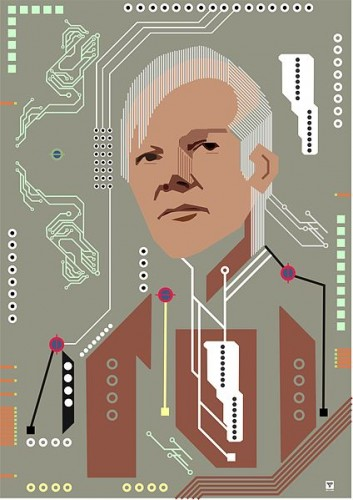
\includegraphics[width=.7\linewidth]{Pictures/assange.jpg}
\end{center}
\end{block}
\end{column}
\end{columns}
\end{block}

\begin{block}{La Naissance du Bitcoin}
\begin{block}{Cypherpunk (Hal Finney)}
\begin{center}
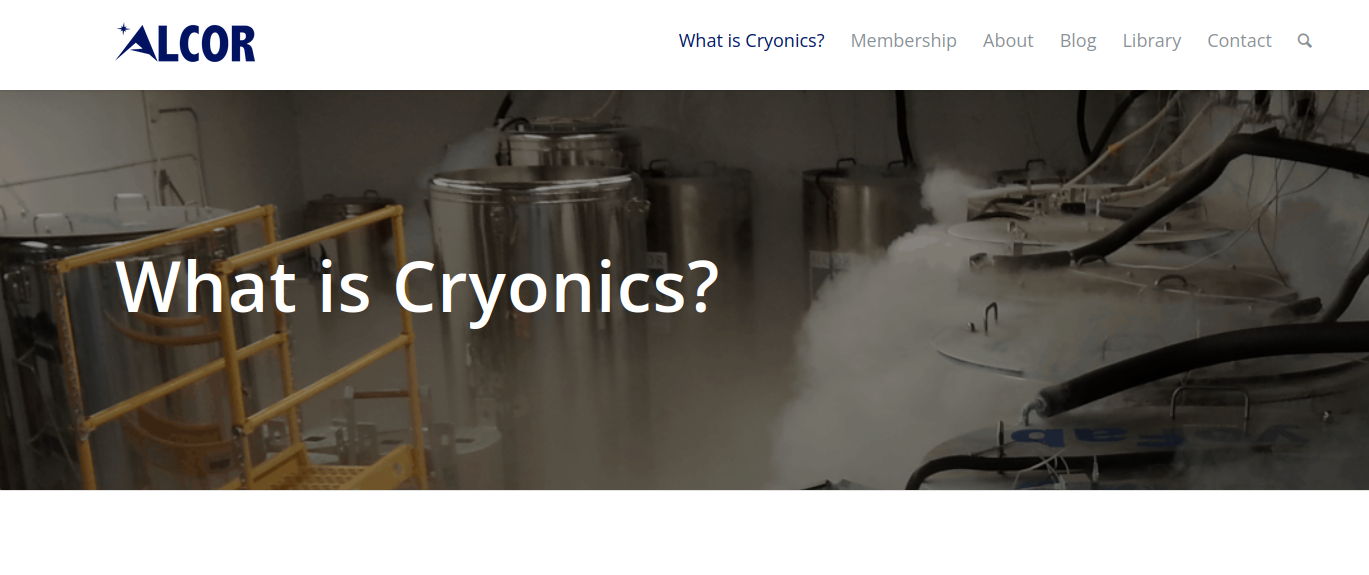
\includegraphics[width=\linewidth]{Pictures/cryonics_hal_finney.png}
\end{center}
\end{block}
\end{block}
\end{frame}

\begin{frame}[label={sec:org88d23fe}]{Que vaut la blockchain ?}
\begin{block}{Que vaut la blockchain ?}
\begin{center}
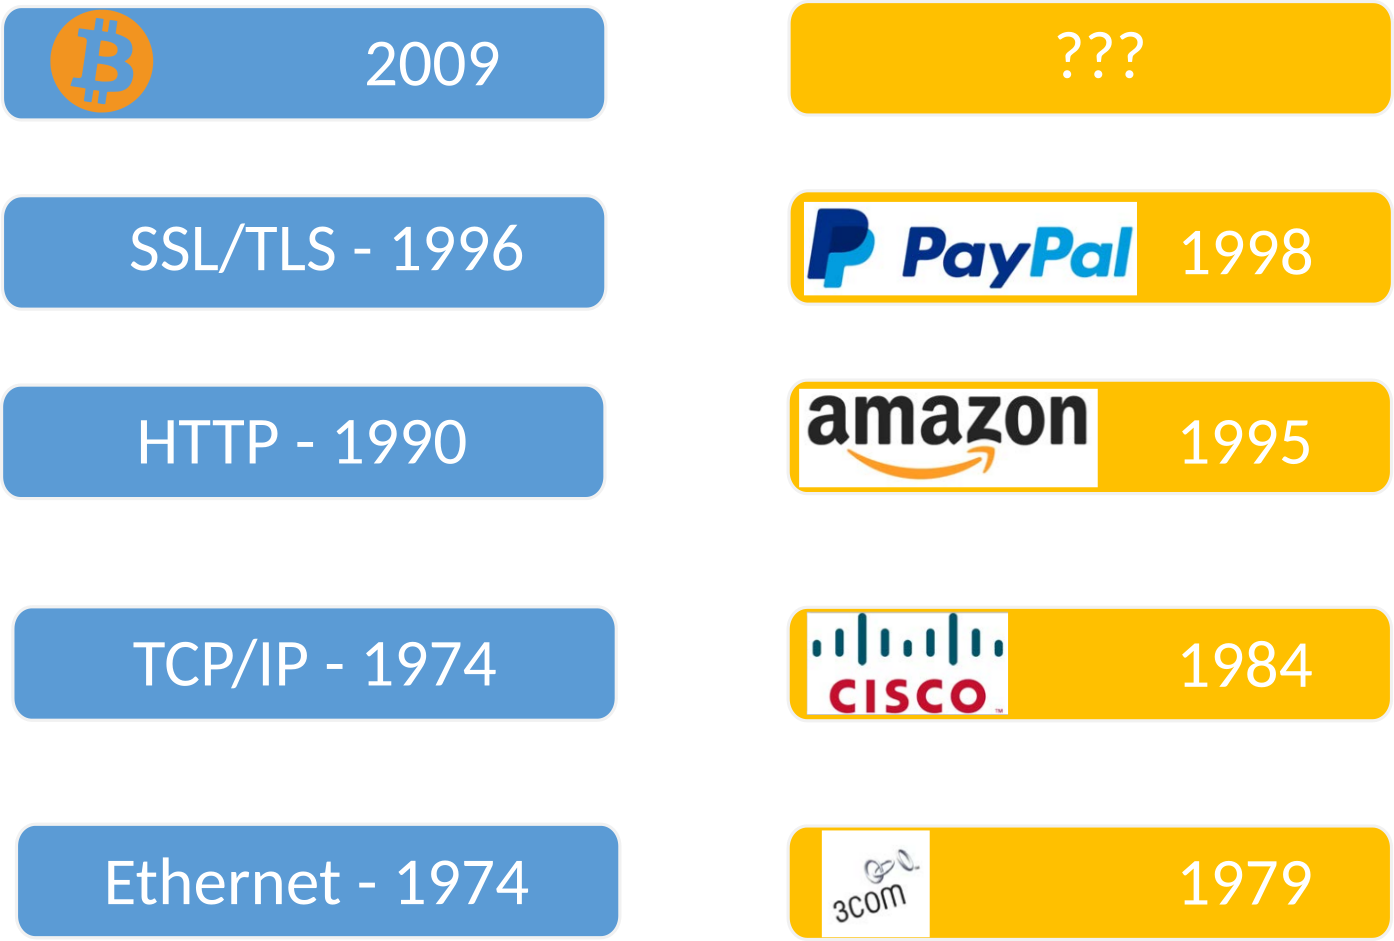
\includegraphics[width=.8\linewidth]{Pictures/layers_btc.png}
\end{center}
\begin{block}{Cela dépendera de son utilité}
\end{block}
\end{block}
\end{frame}

\begin{frame}[label={sec:org6ff9387}]{Historique du cours du Bitcoin}
\begin{block}{}
\begin{center}
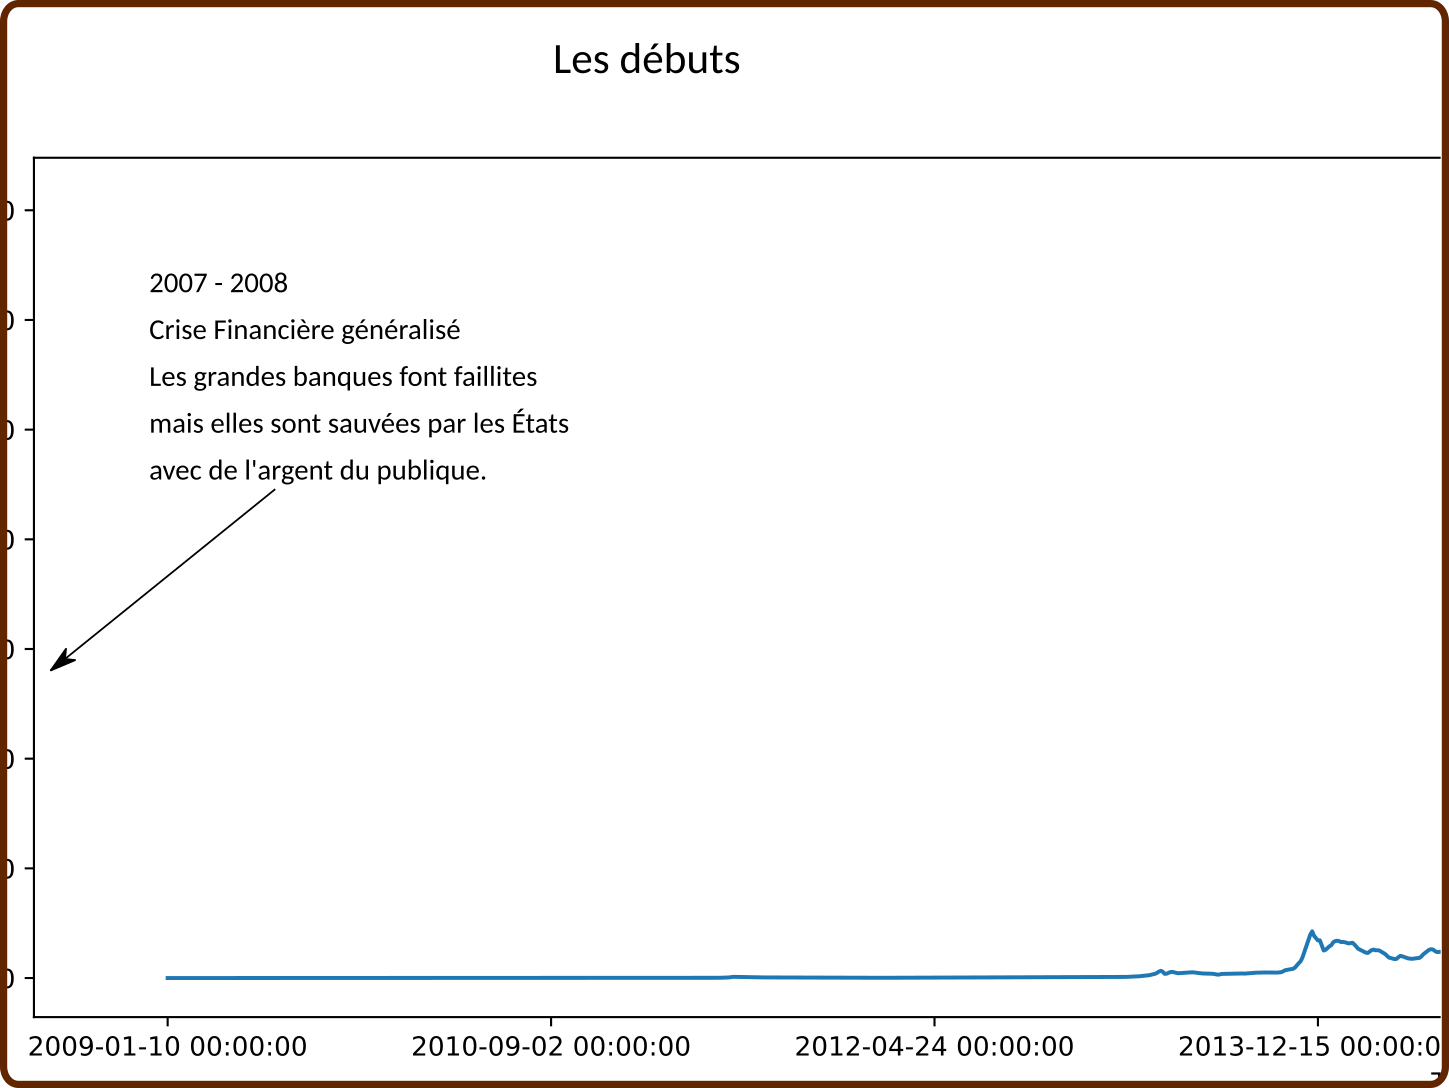
\includegraphics[width=.95\textwidth]{./Pictures/Timeline/00debut0.png}
\end{center}
\end{block}
\begin{block}{}
\begin{center}
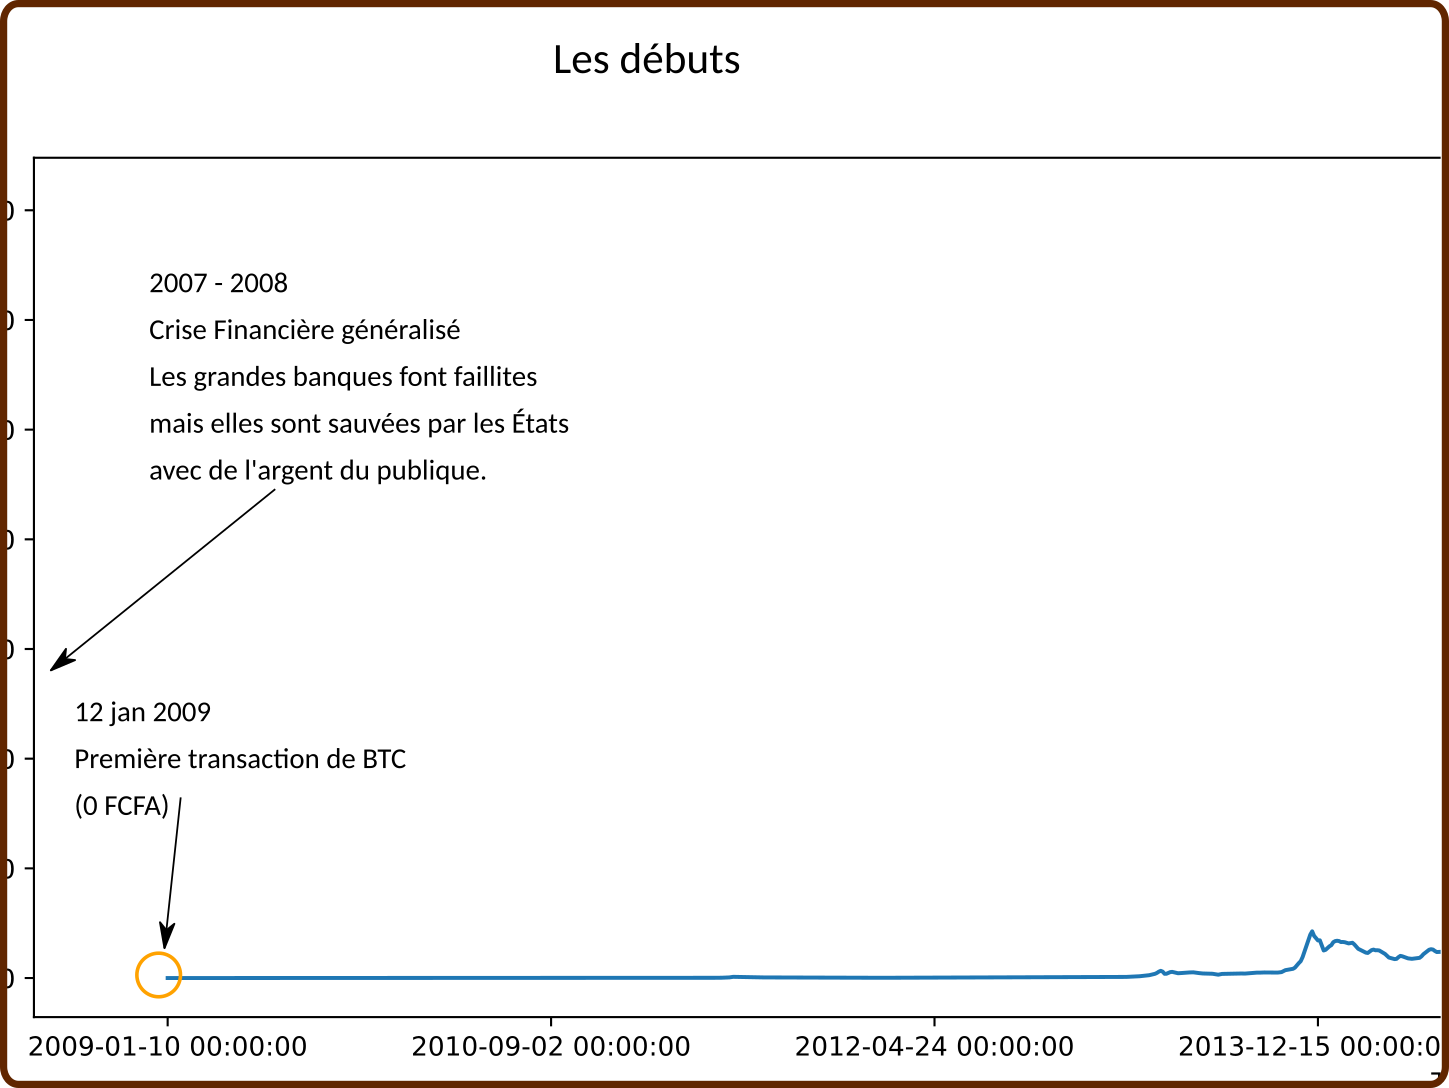
\includegraphics[width=.95\textwidth]{./Pictures/Timeline/01debut_prix_crea.png}
\end{center}
\end{block}

\begin{block}{}
\begin{center}
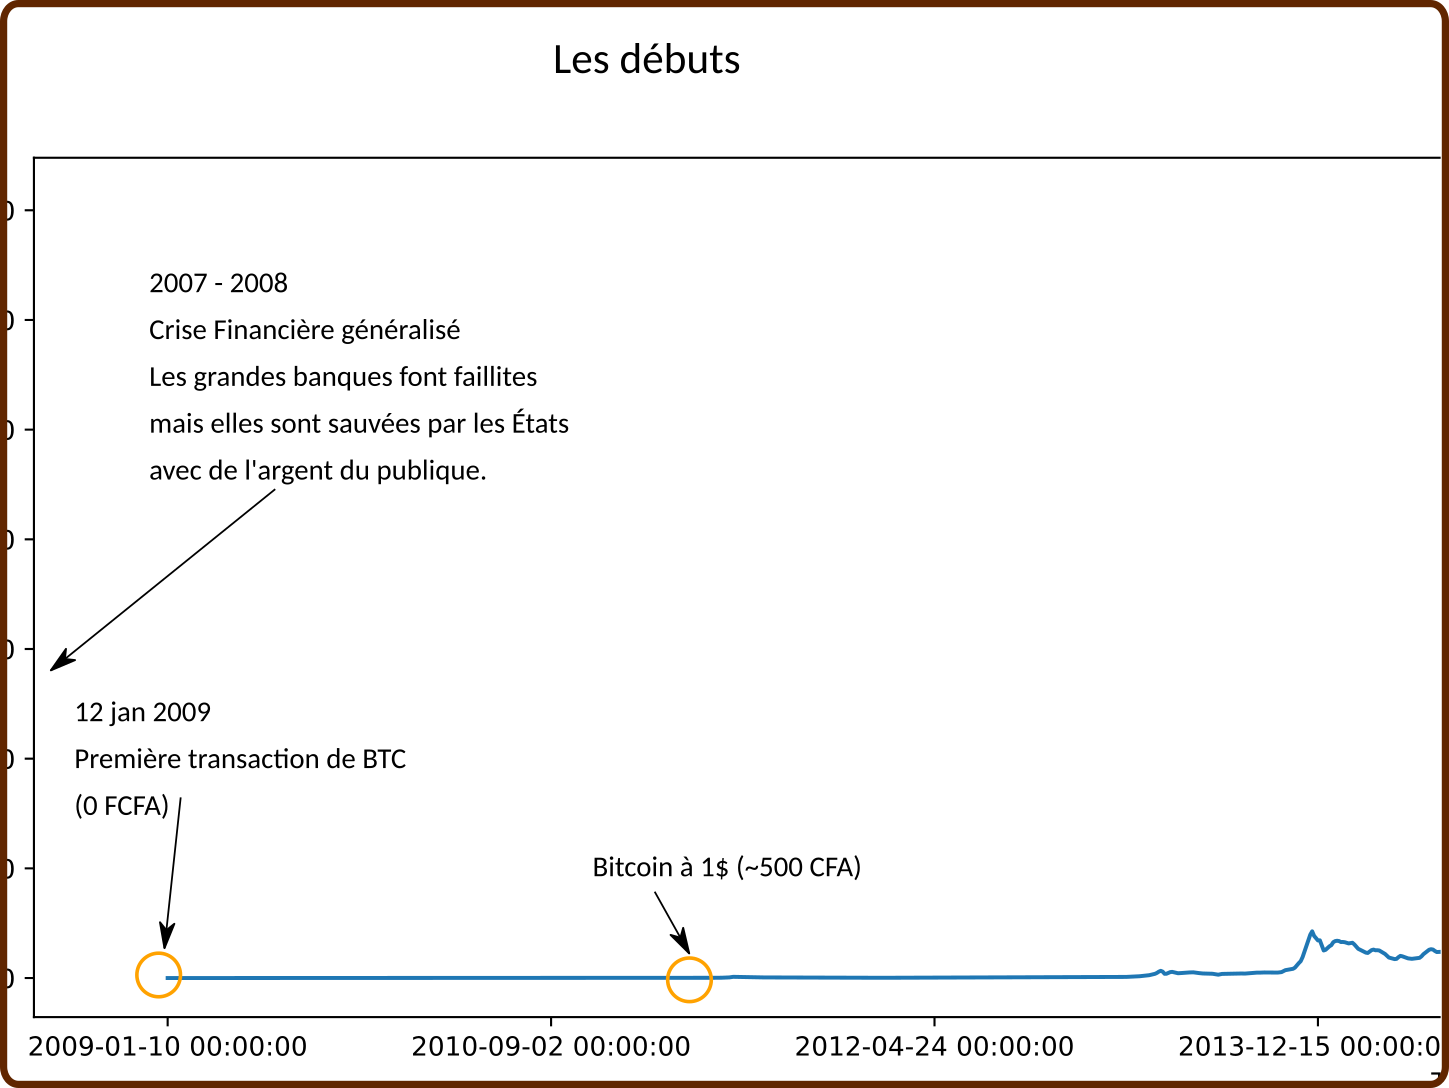
\includegraphics[width=.95\textwidth]{./Pictures/Timeline/02debut_prix_1.png}
\end{center}
\end{block}
\begin{block}{}
\begin{center}
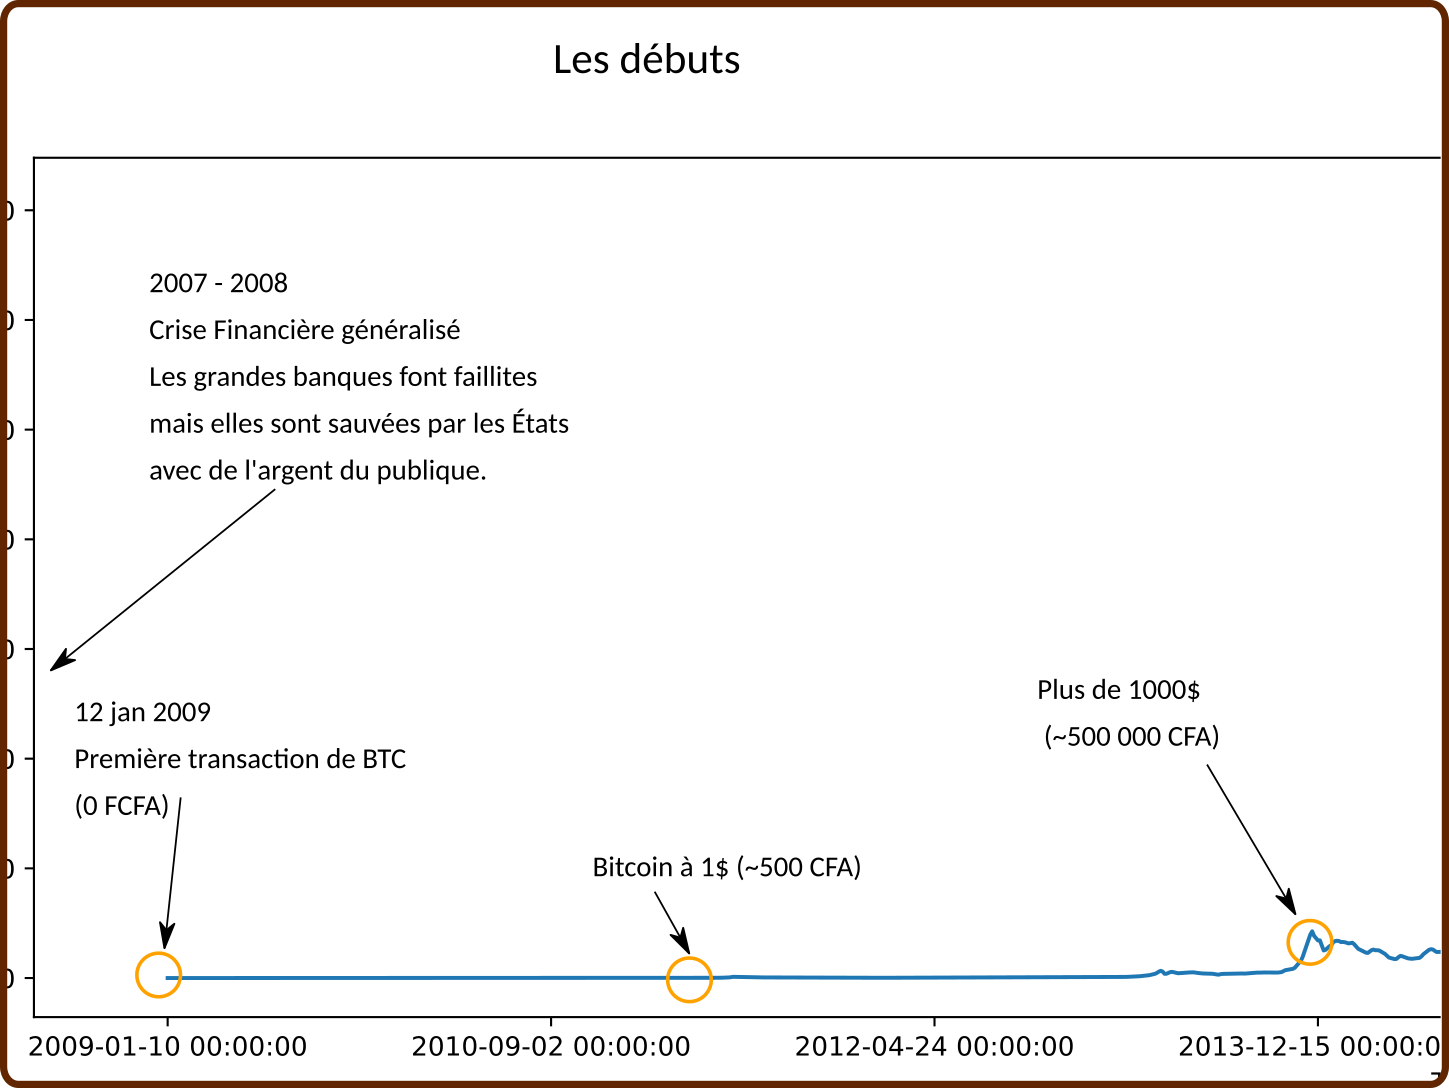
\includegraphics[width=.95\textwidth]{./Pictures/Timeline/03debut_prix_1000.png}
\end{center}
\end{block}
\begin{block}{}
\begin{center}
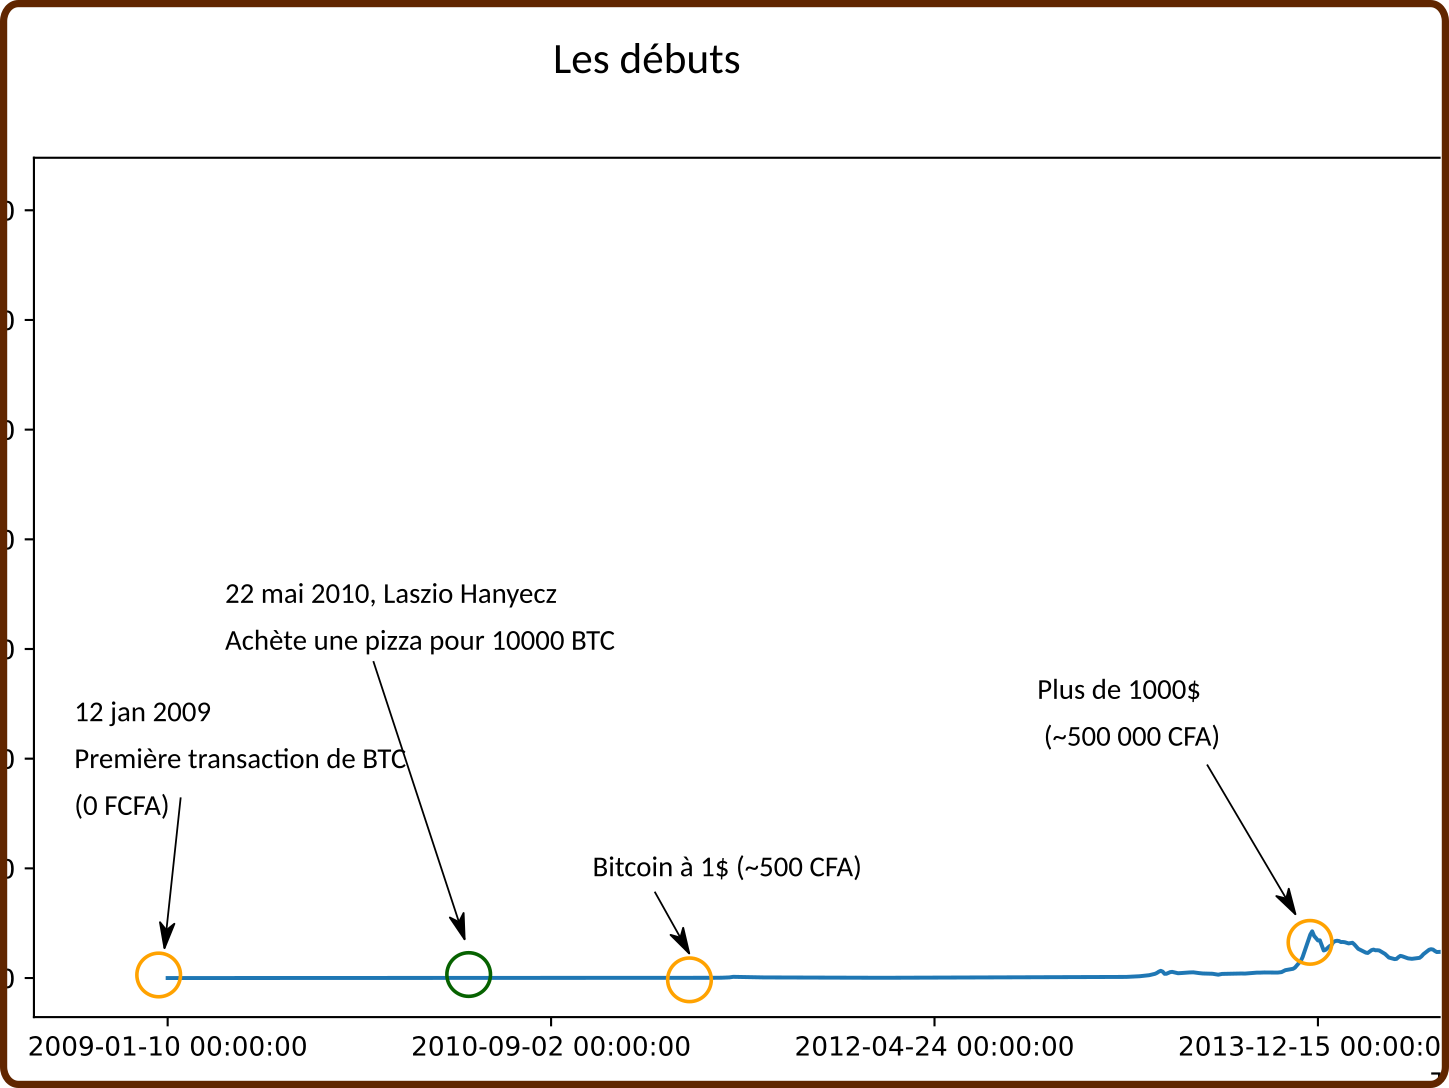
\includegraphics[width=.95\textwidth]{./Pictures/Timeline/04debut_pizza.png}
\end{center}
\end{block}

\begin{block}{}
\begin{center}
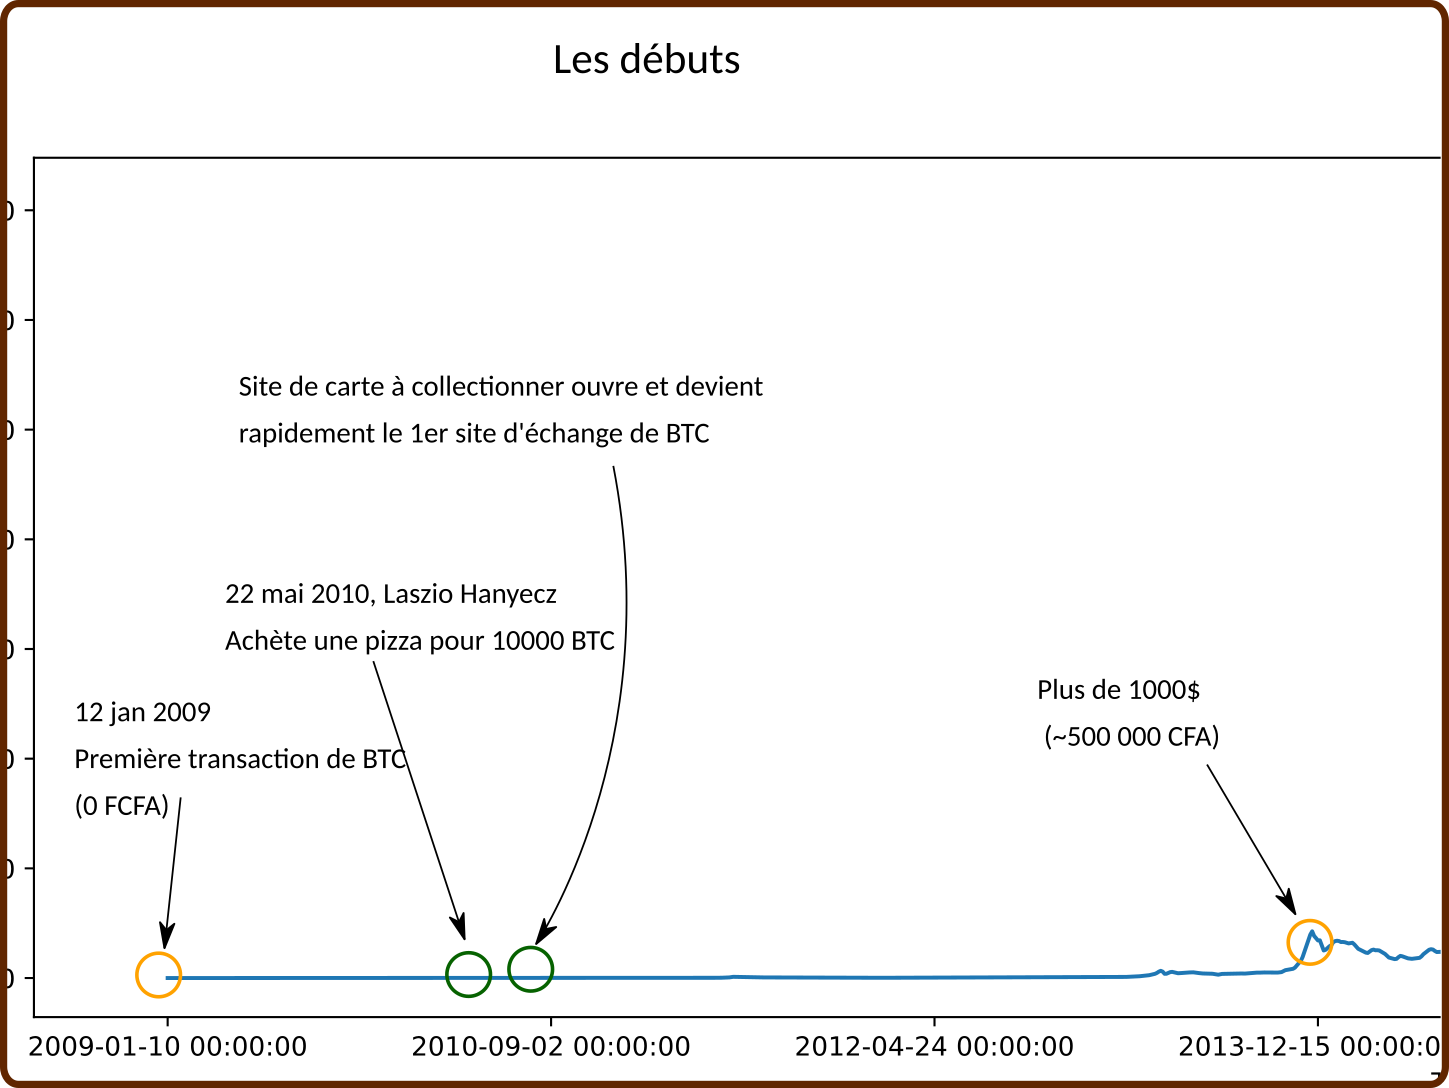
\includegraphics[width=.95\textwidth]{./Pictures/Timeline/05debut_mtdox.png}
\end{center}
\end{block}

\begin{block}{}
\begin{center}
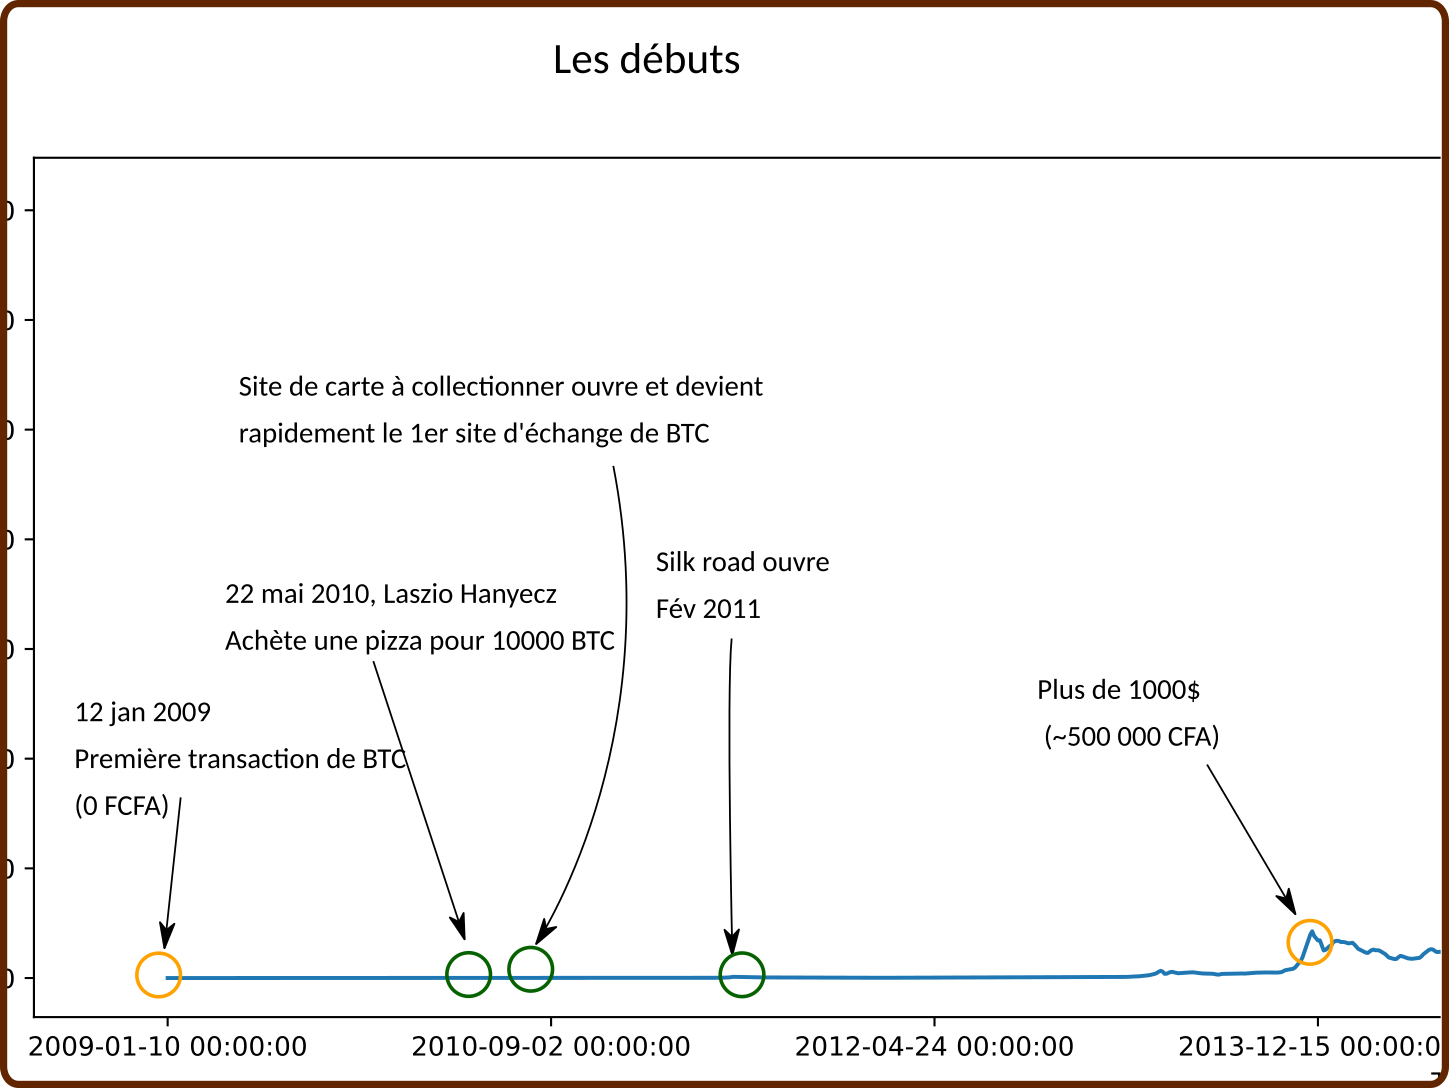
\includegraphics[width=.95\textwidth]{./Pictures/Timeline/06debut_silk.png}
\end{center}
\end{block}

\begin{block}{}
\begin{center}
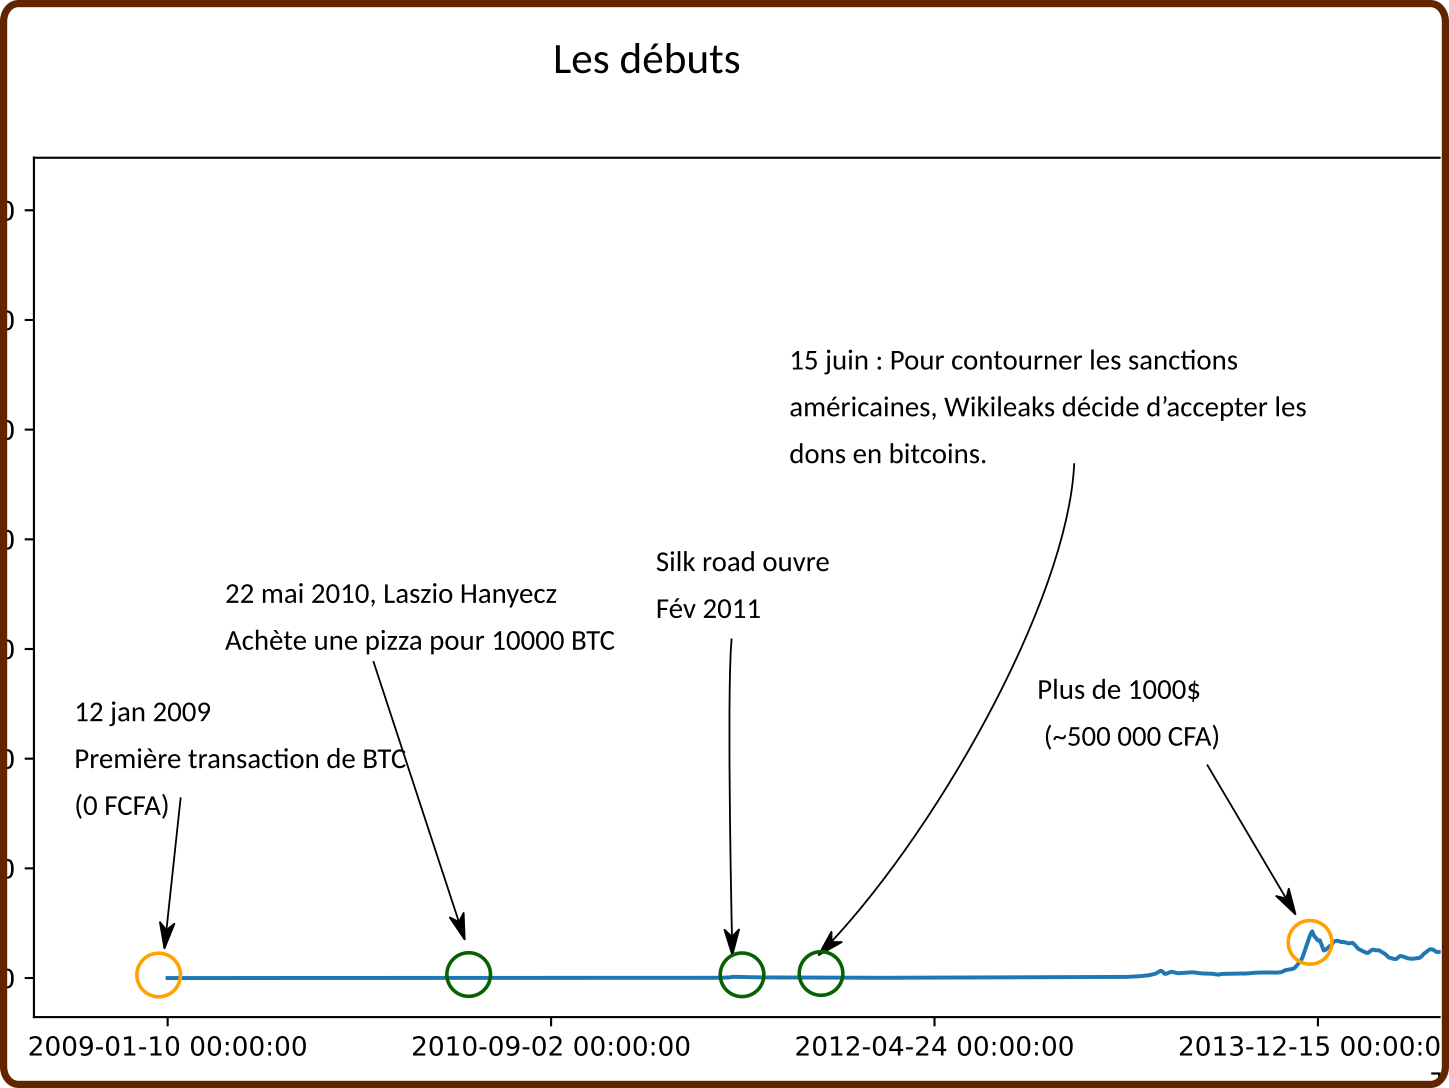
\includegraphics[width=.95\textwidth]{./Pictures/Timeline/07debut_wiki.png}
\end{center}
\end{block}

\begin{block}{}
\begin{center}
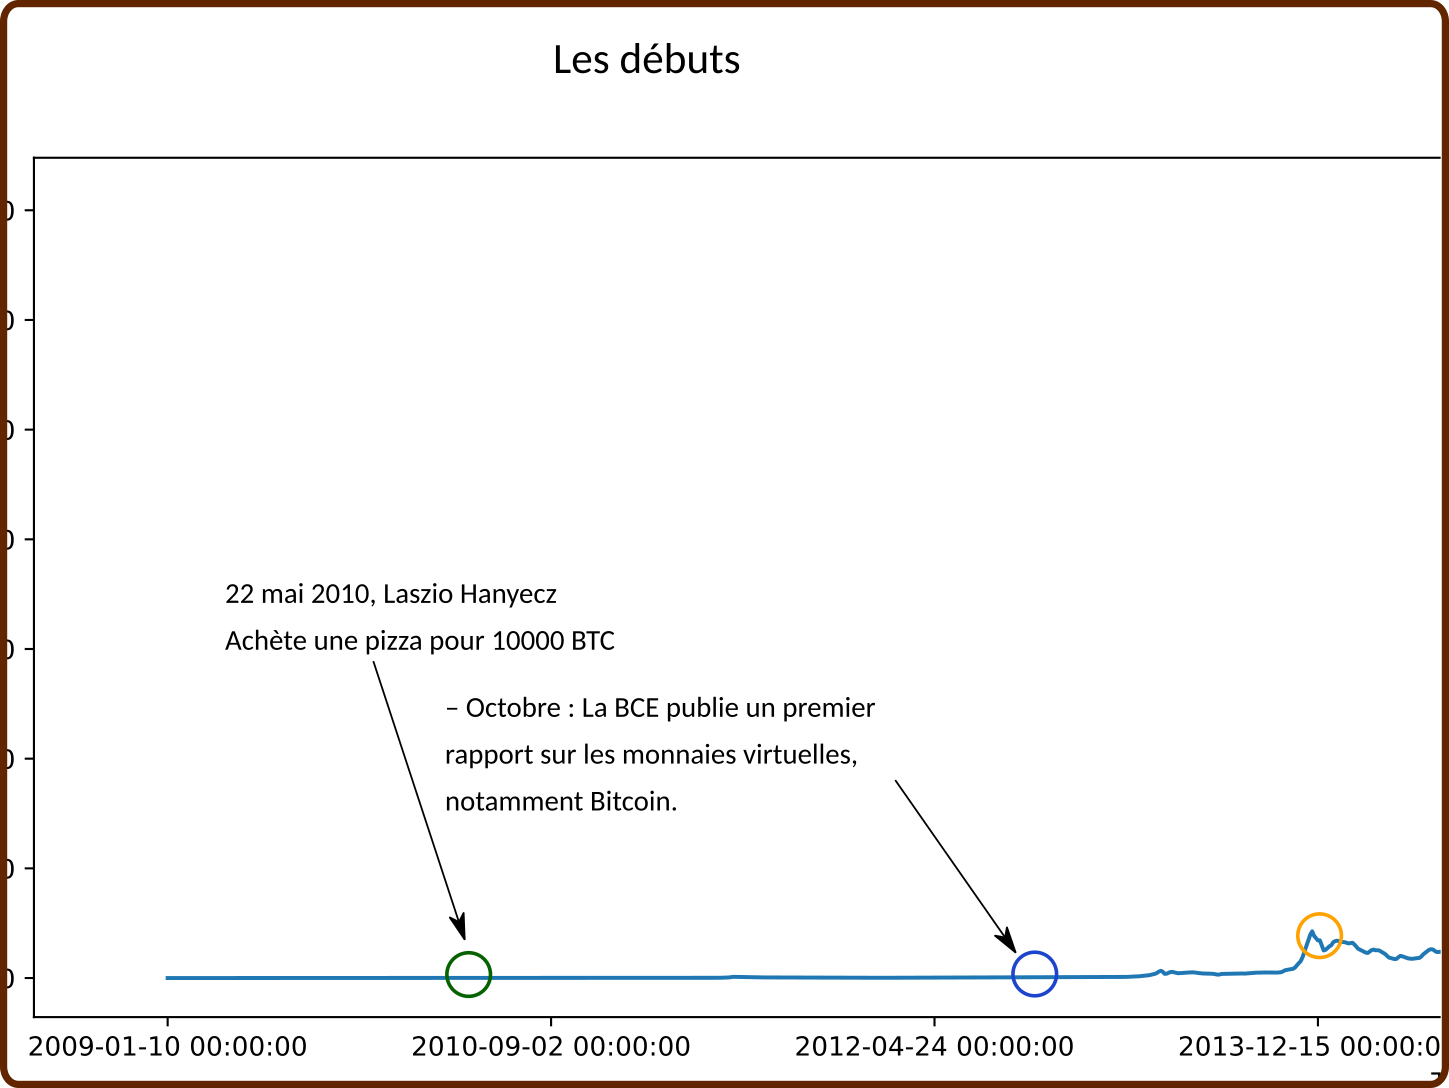
\includegraphics[width=.95\textwidth]{./Pictures/Timeline/10debut_BCE.png}
\end{center}
\end{block}

\begin{block}{}
\begin{center}
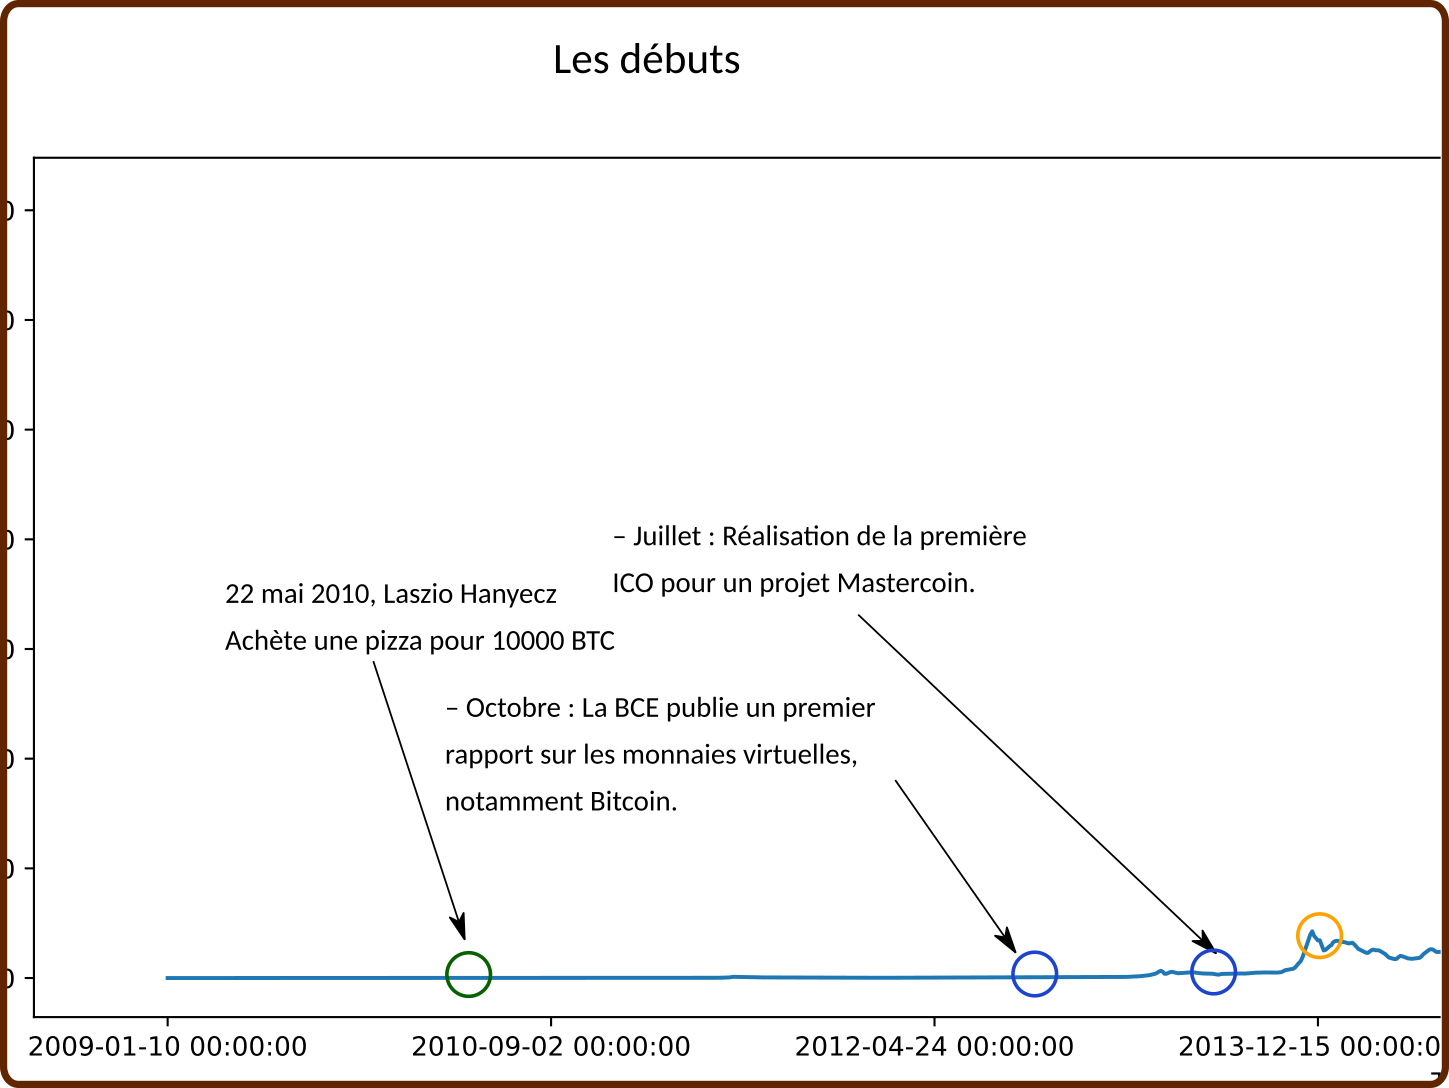
\includegraphics[width=.95\textwidth]{./Pictures/Timeline/11debut_ICO.png}
\end{center}
\end{block}

\begin{block}{}
\begin{center}
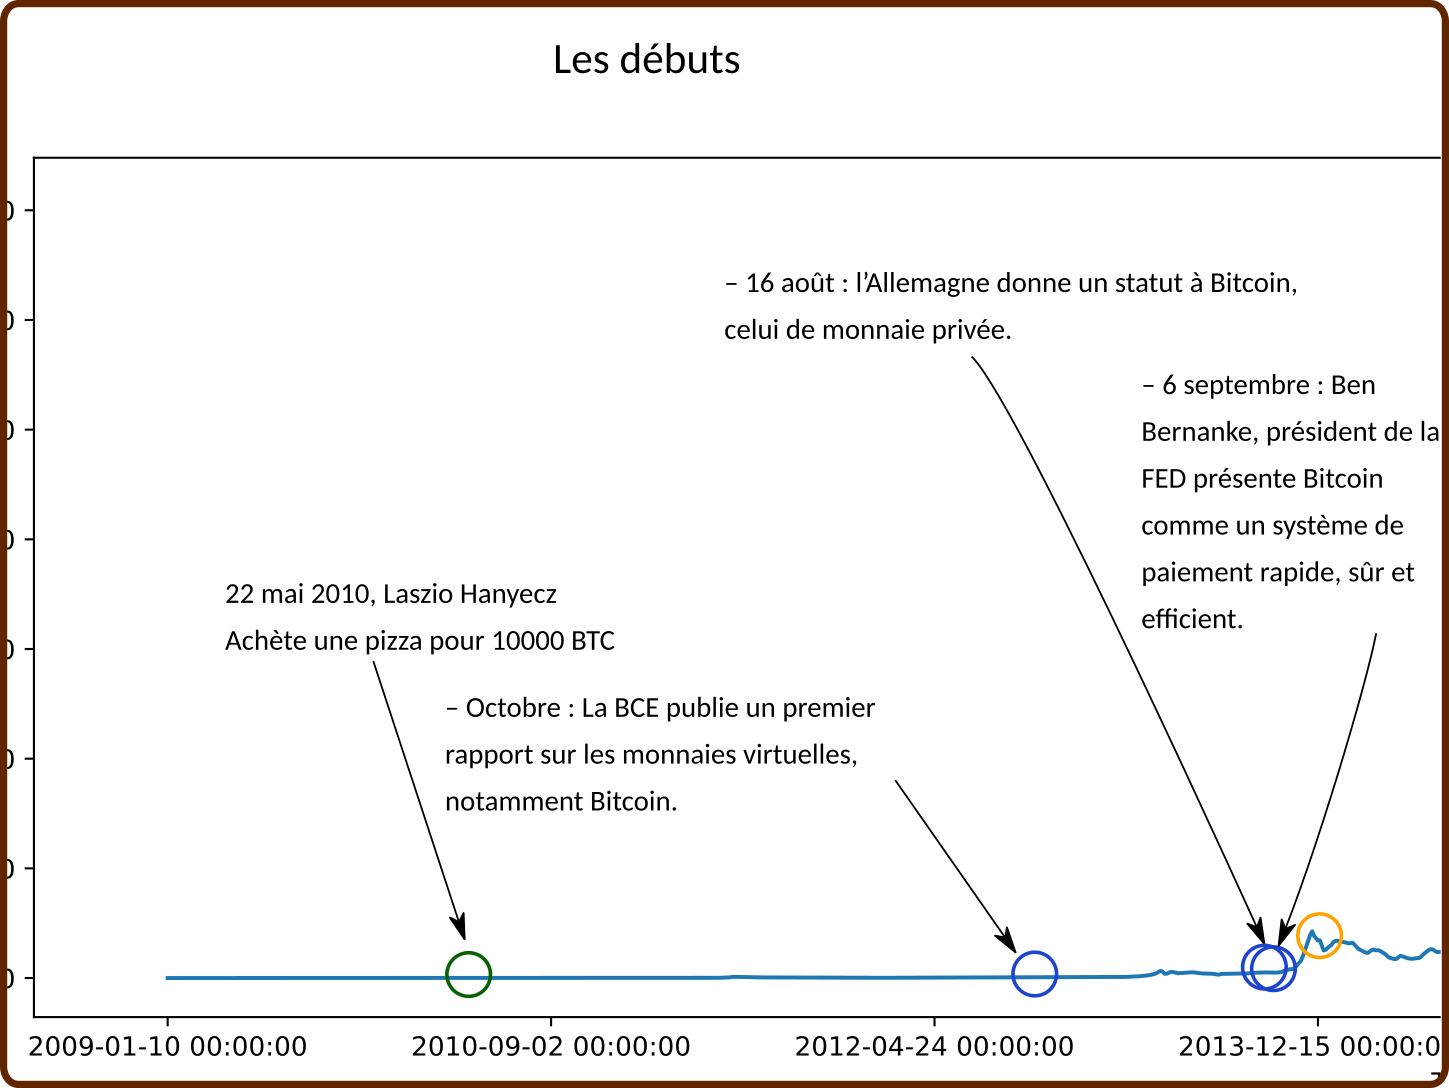
\includegraphics[width=.95\textwidth]{./Pictures/Timeline/12debut_FED.png}
\end{center}
\end{block}

\begin{block}{}
\begin{center}
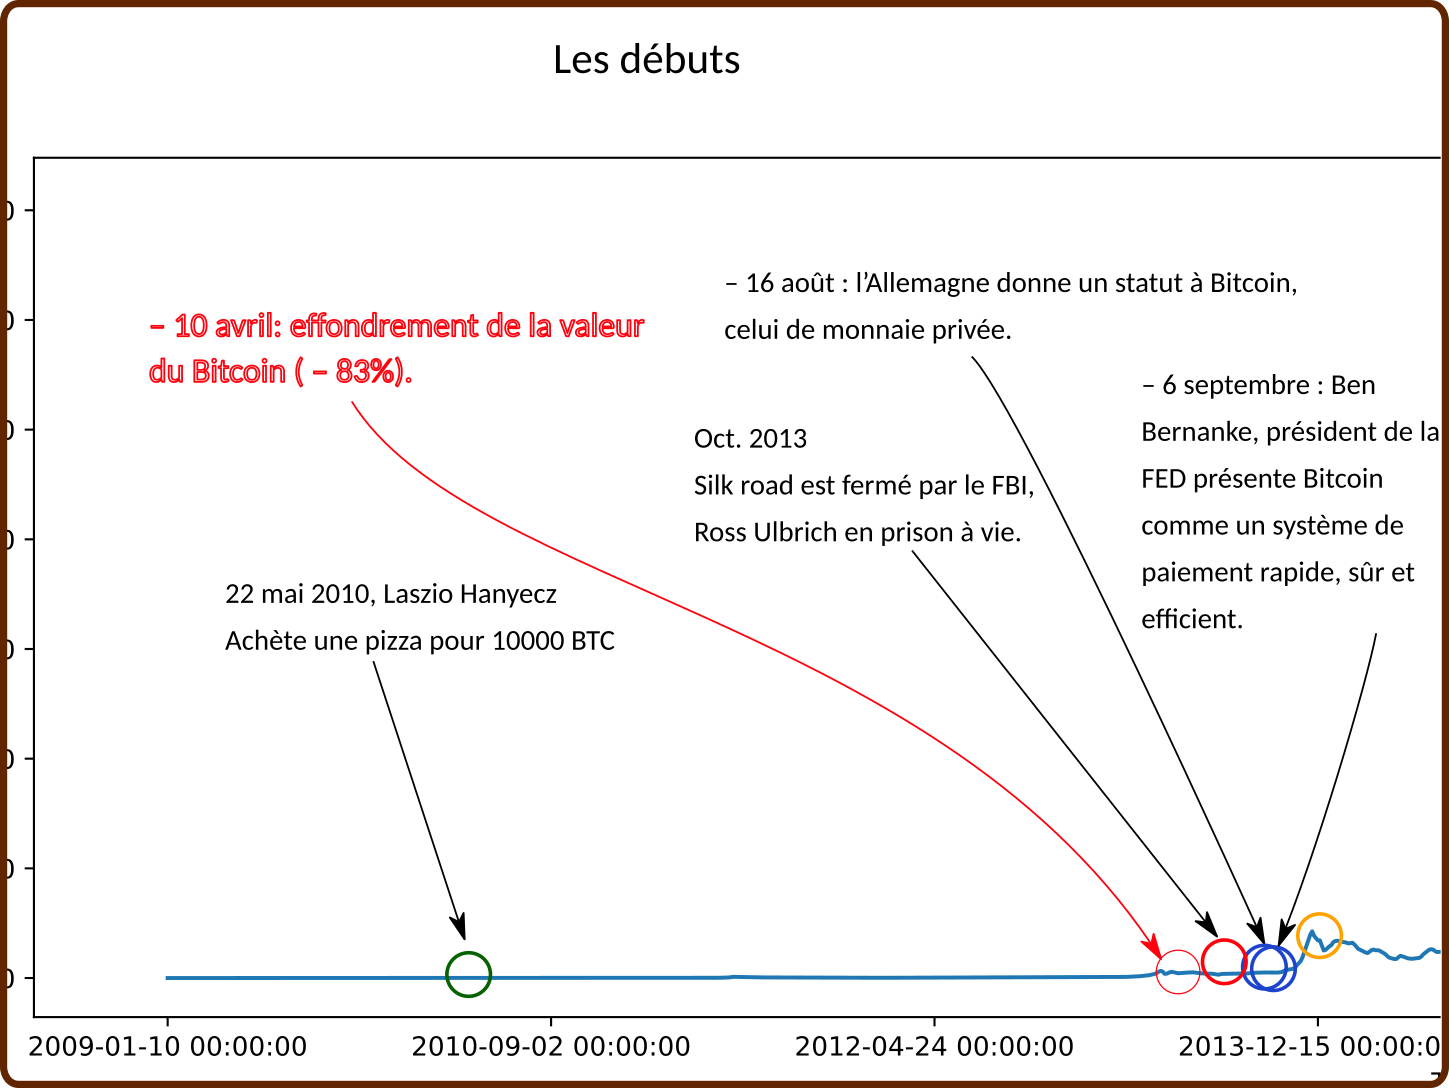
\includegraphics[width=.95\textwidth]{./Pictures/Timeline/13debut_realite.png}
\end{center}
\end{block}

\begin{block}{}
\begin{center}
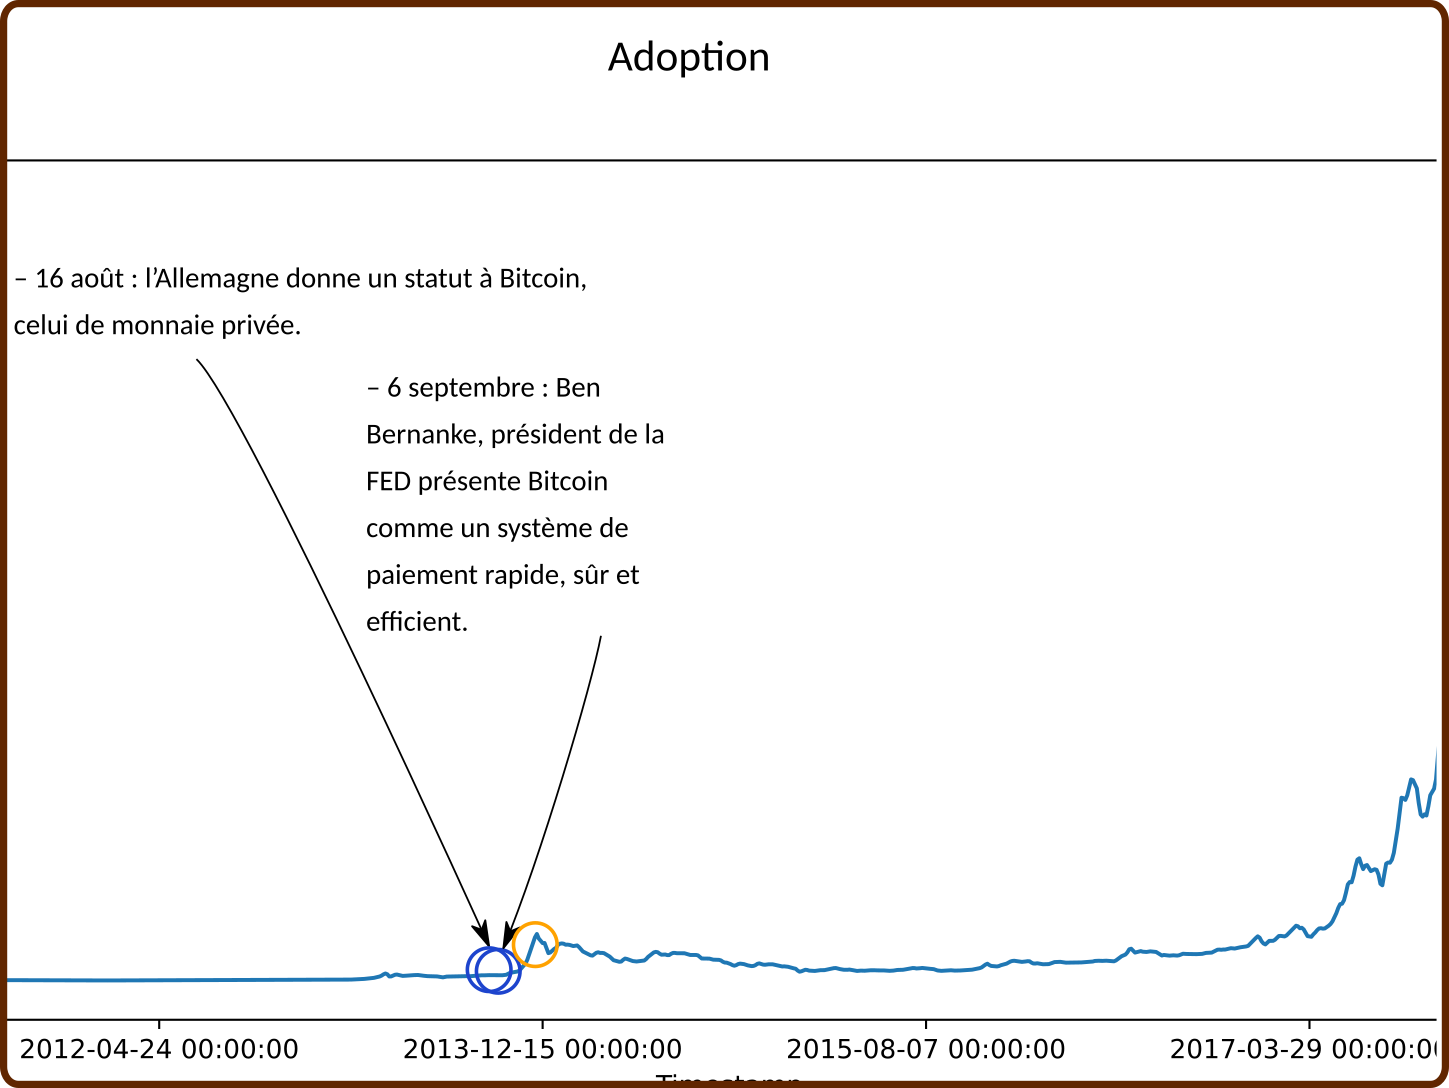
\includegraphics[width=.95\textwidth]{./Pictures/Timeline/20adoption.png}
\end{center}
\end{block}

\begin{block}{}
\begin{center}
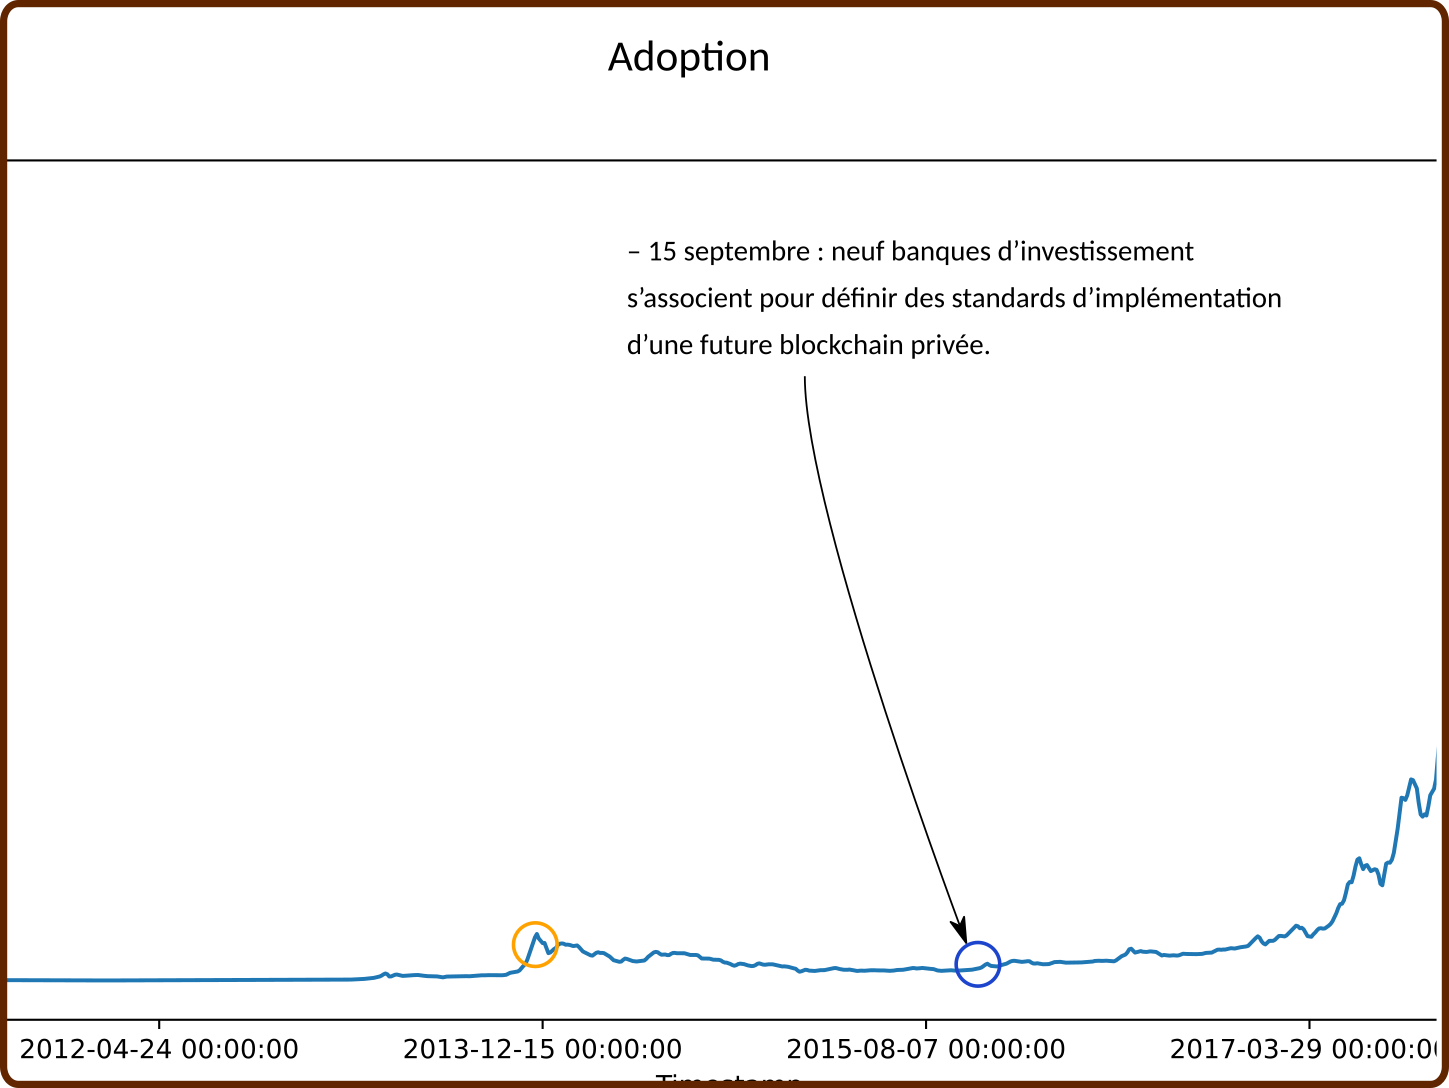
\includegraphics[width=.95\textwidth]{./Pictures/Timeline/21adoption_blockchain_privee.png}
\end{center}
\end{block}

\begin{block}{}
\begin{center}
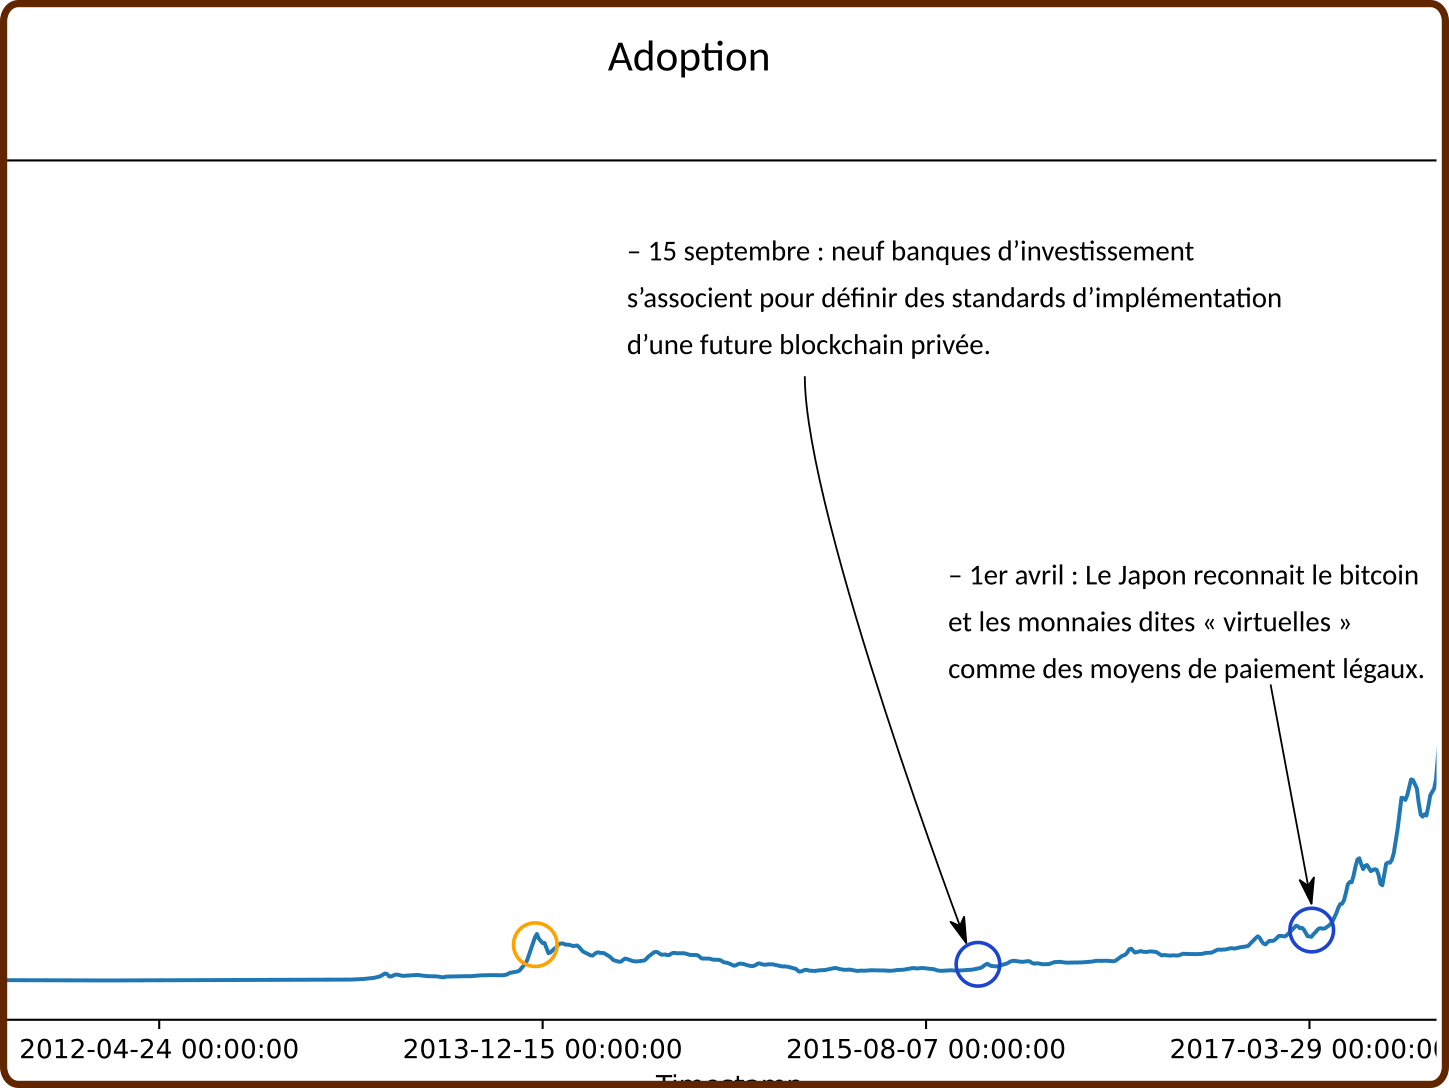
\includegraphics[width=.95\textwidth]{./Pictures/Timeline/21adoption_japon.png}
\end{center}
\end{block}

\begin{block}{}
\begin{center}
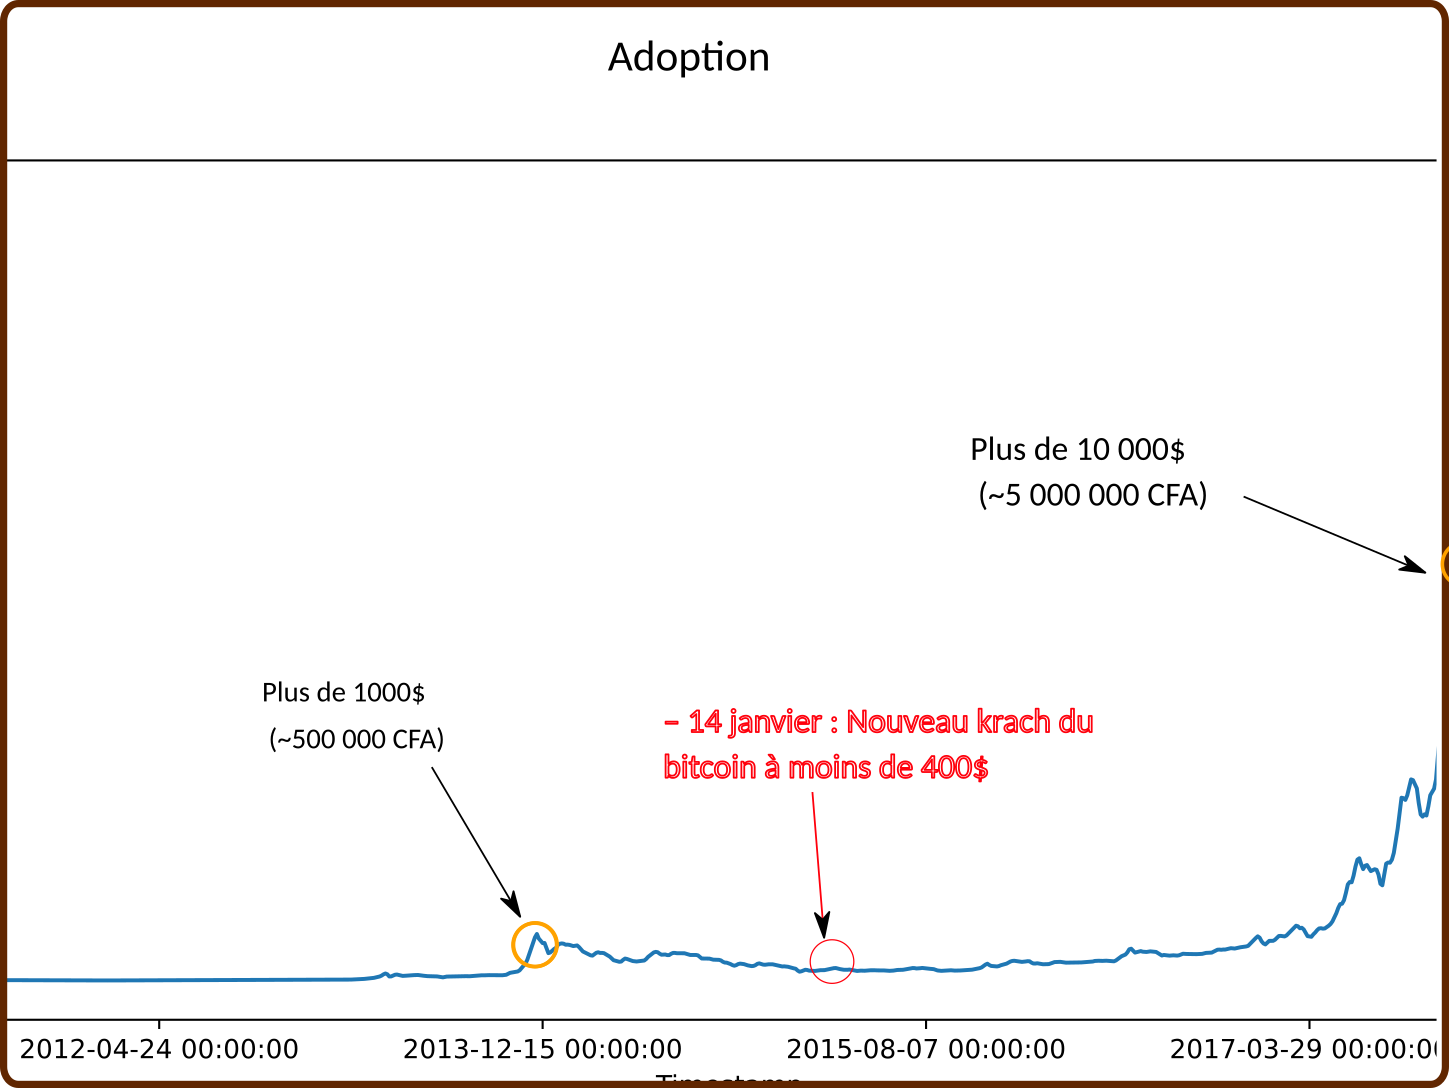
\includegraphics[width=.95\textwidth]{./Pictures/Timeline/22adoption_prix.png}
\end{center}
\end{block}

\begin{block}{}
\begin{center}
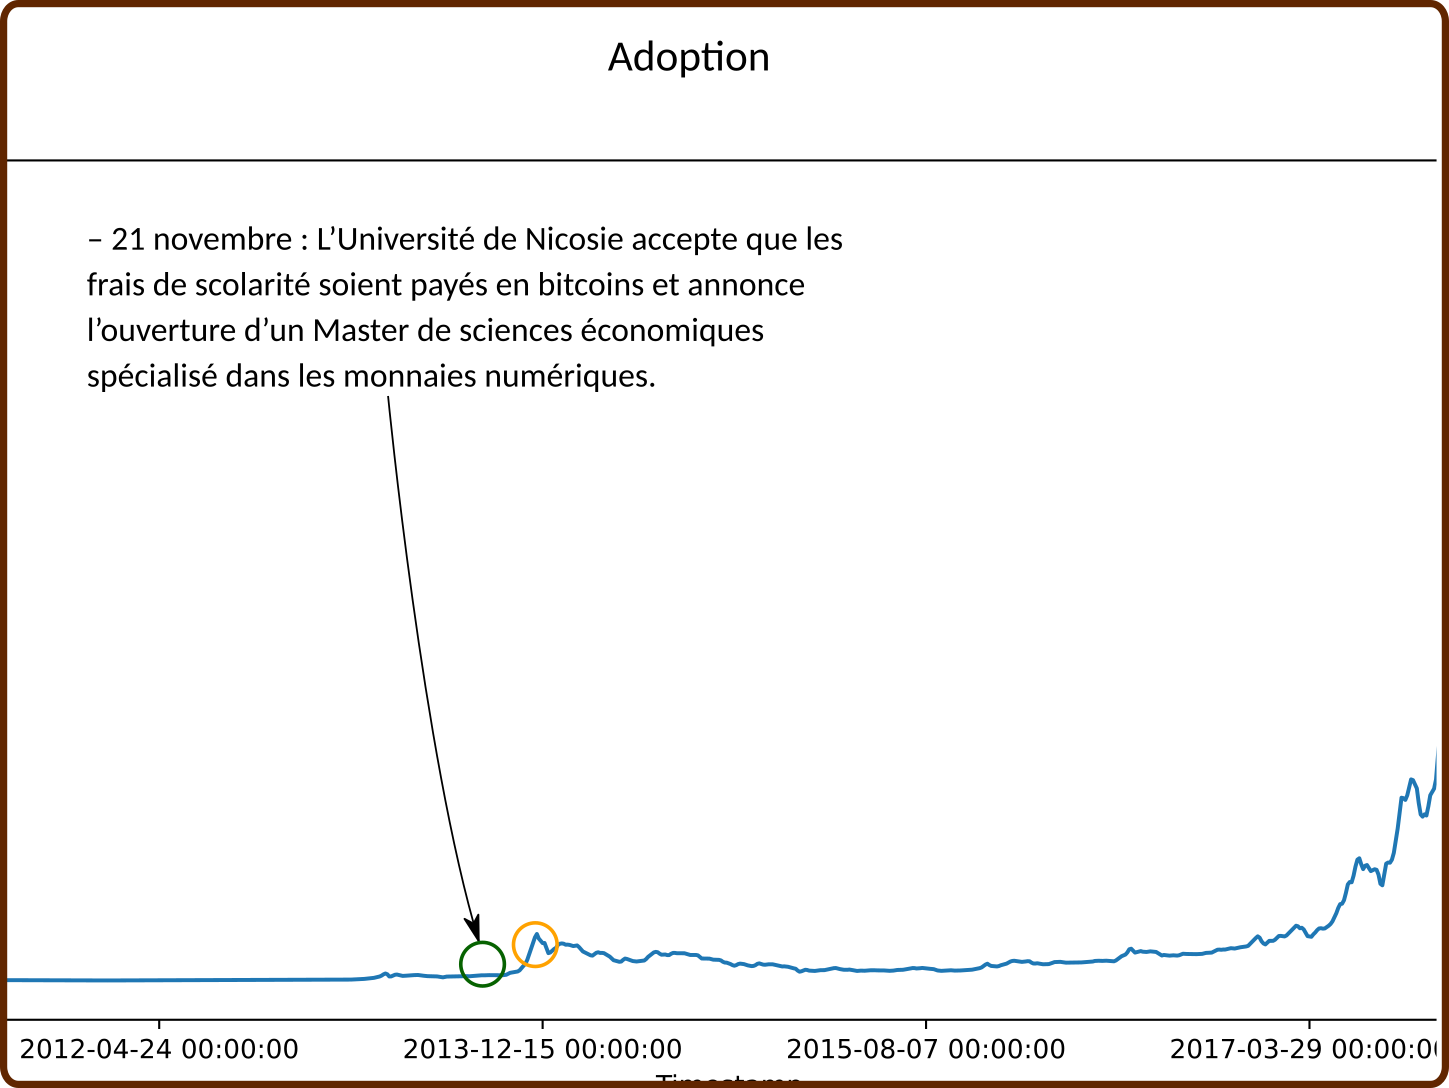
\includegraphics[width=.95\textwidth]{./Pictures/Timeline/23adoption_univ.png}
\end{center}
\end{block}

\begin{block}{}
\begin{center}
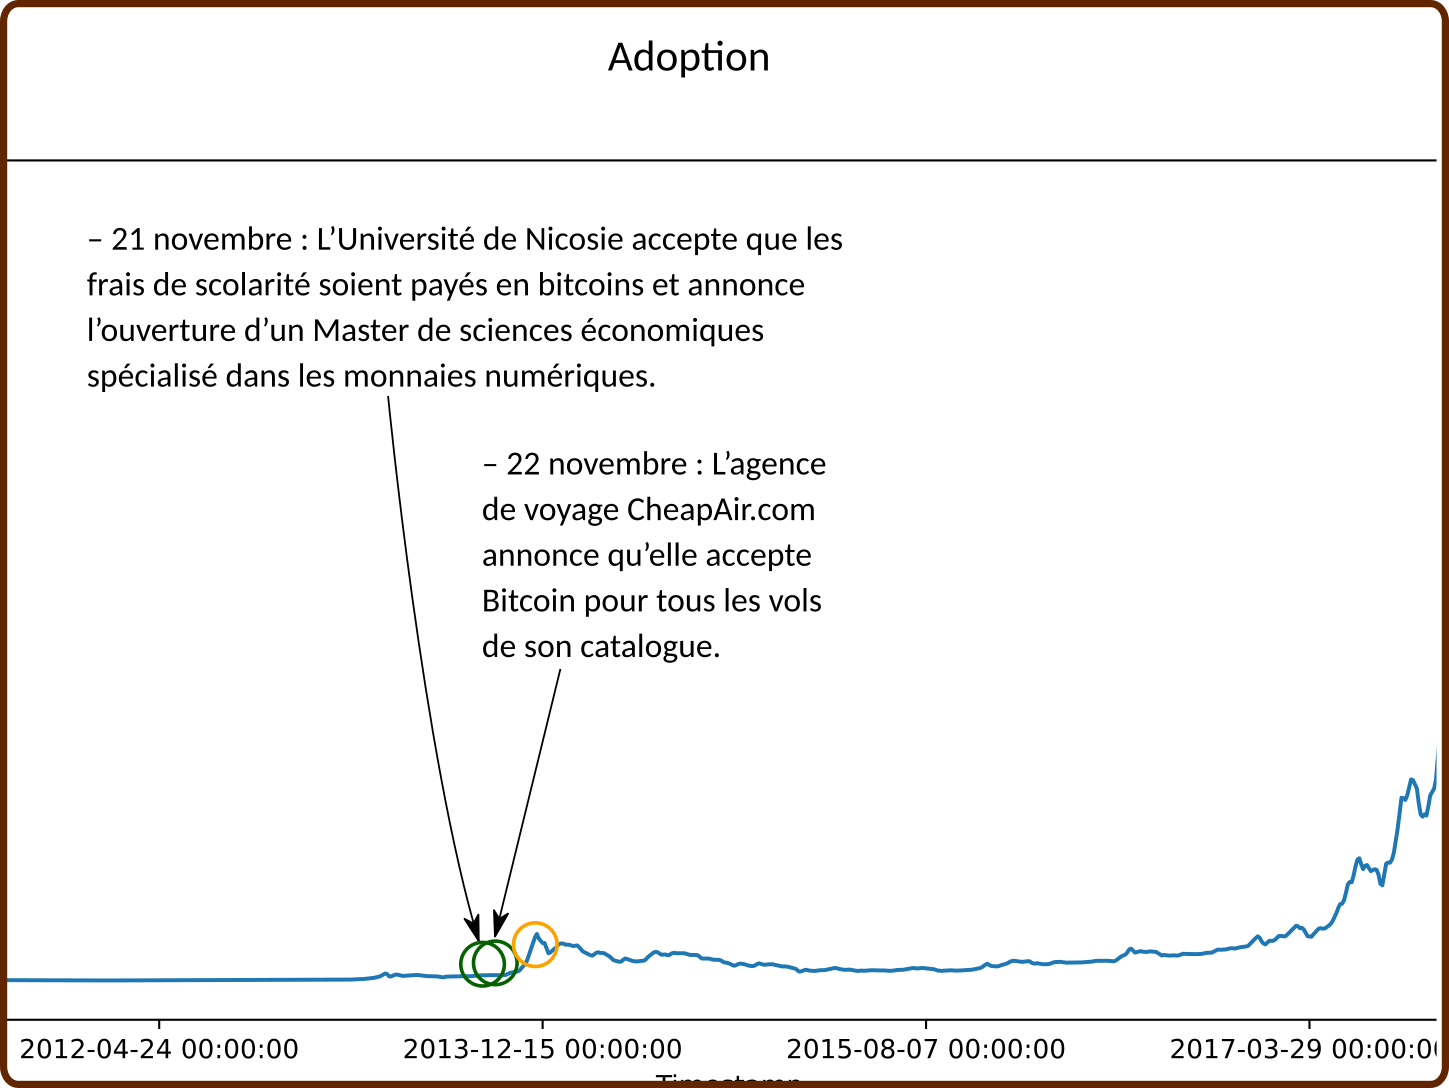
\includegraphics[width=.95\textwidth]{./Pictures/Timeline/23adoption_voyage.png}
\end{center}
\end{block}

\begin{block}{}
\begin{center}
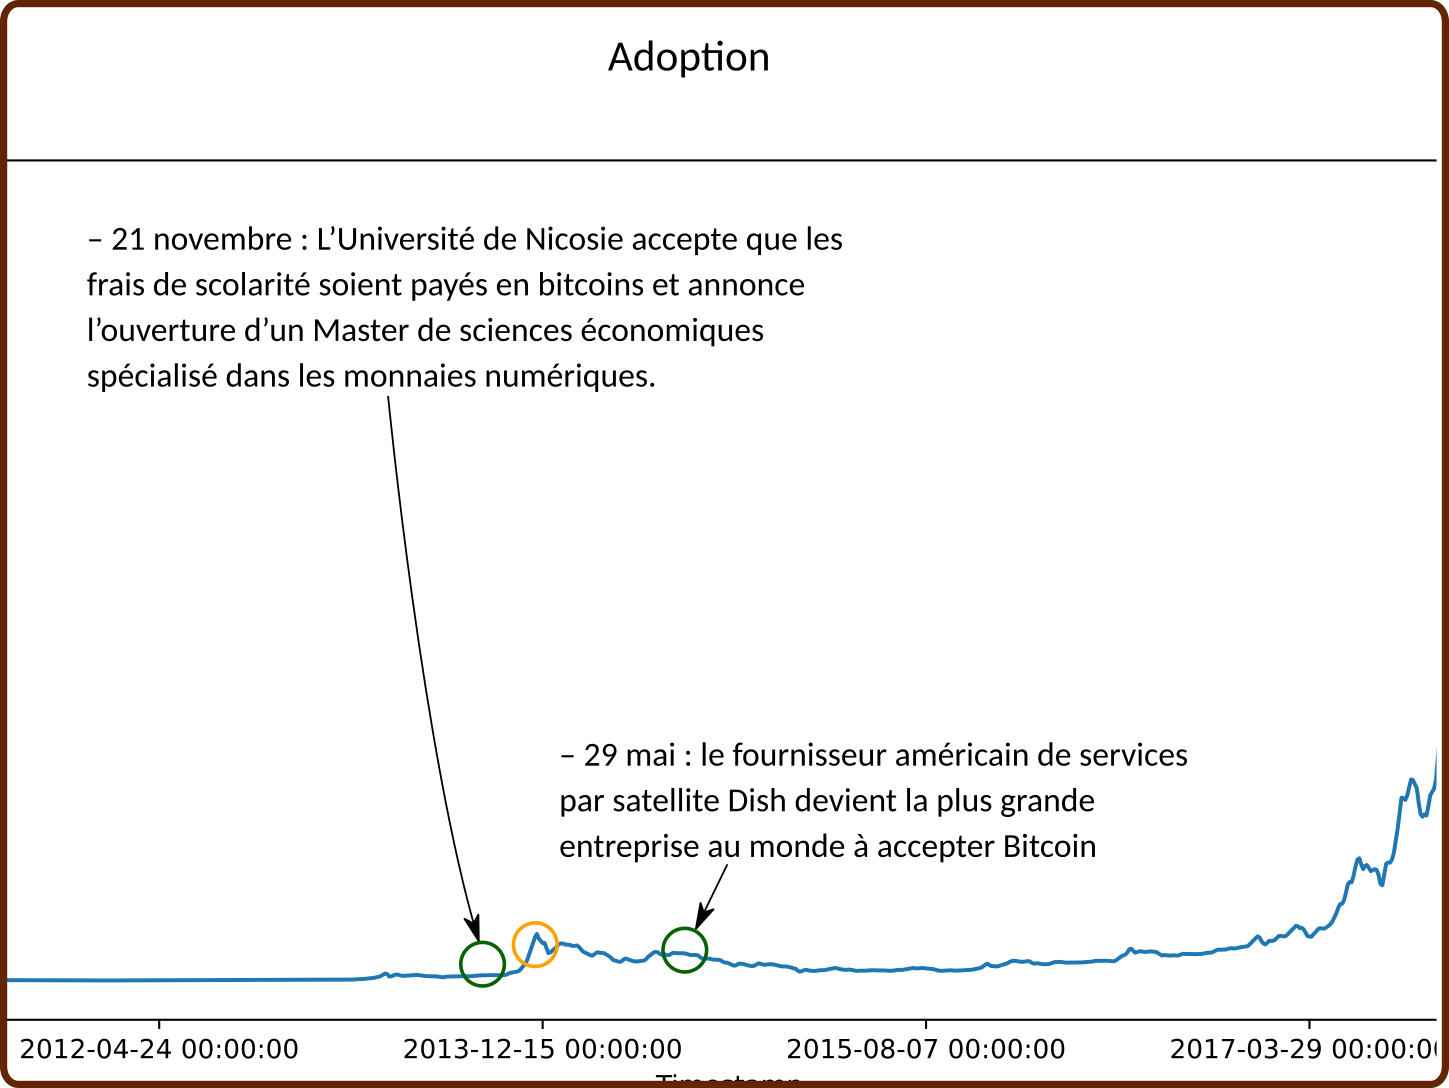
\includegraphics[width=.95\textwidth]{./Pictures/Timeline/24adoption_network.png}
\end{center}
\end{block}

\begin{block}{}
\begin{center}
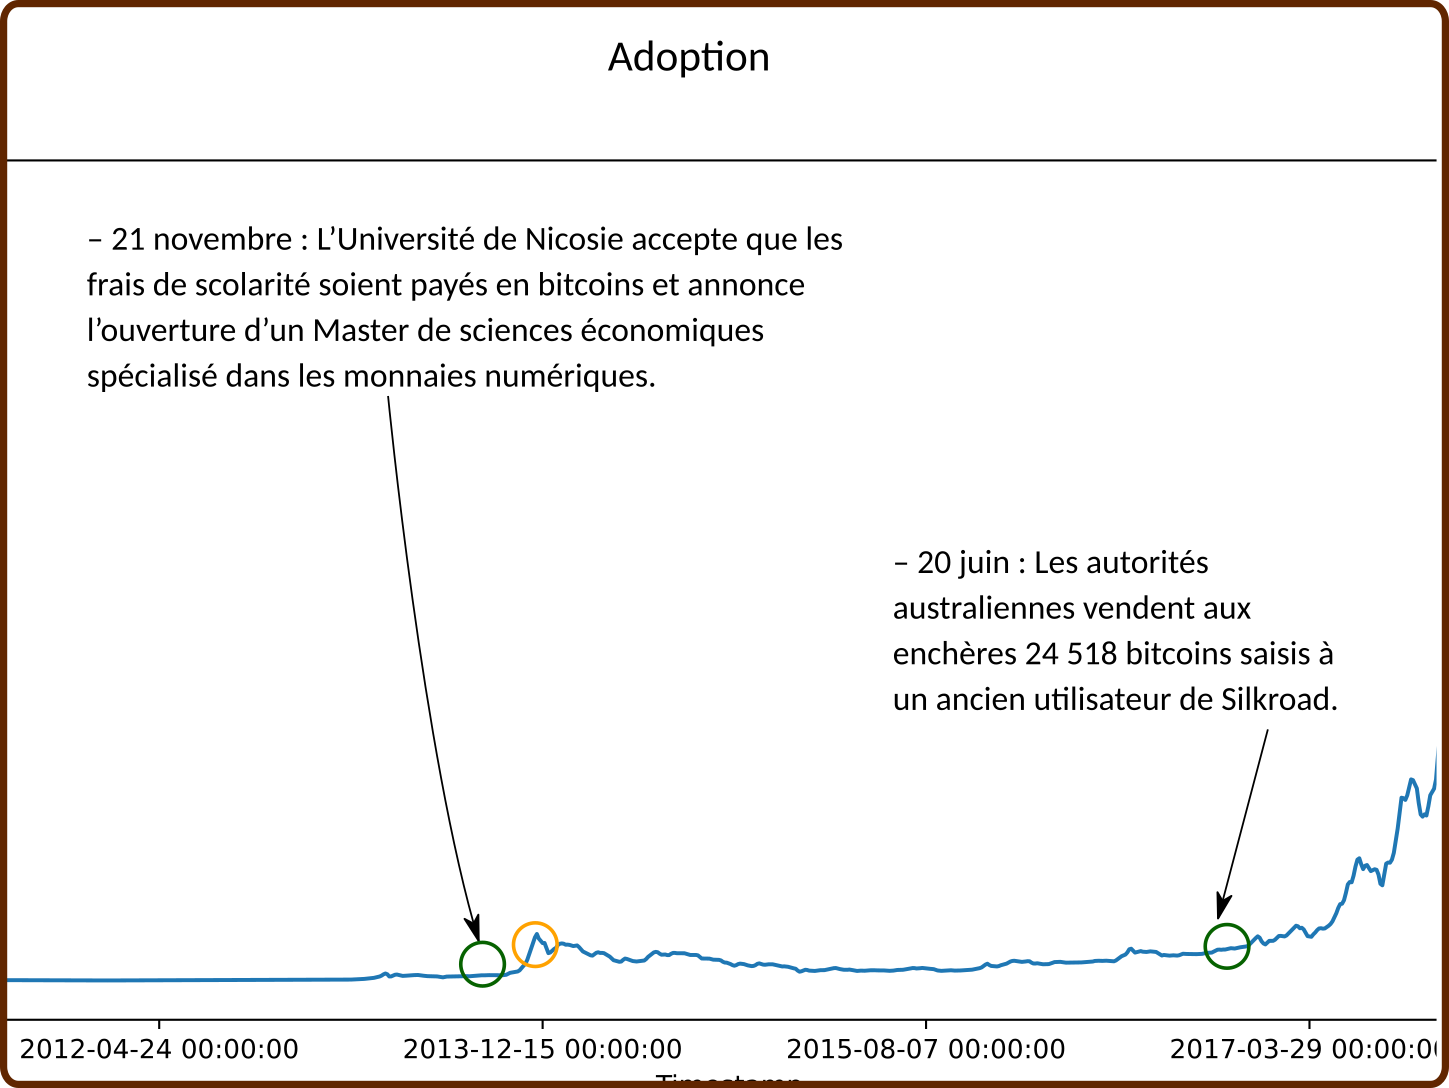
\includegraphics[width=.95\textwidth]{./Pictures/Timeline/25adoption_enchere.png}
\end{center}
\end{block}

\begin{block}{}
\begin{center}
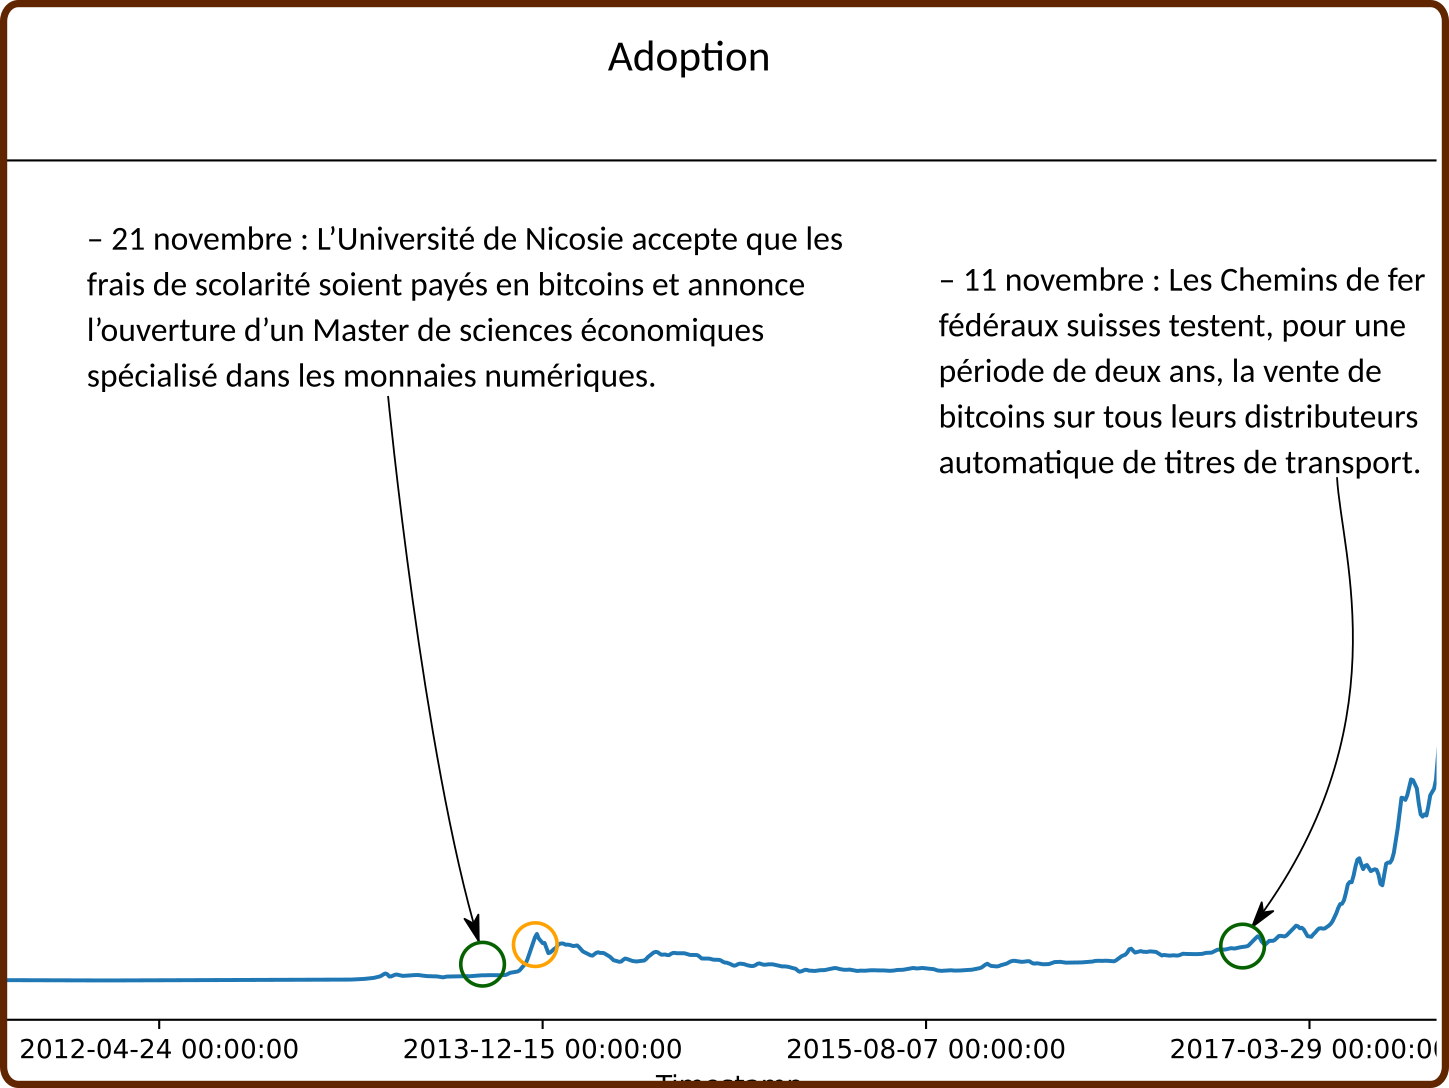
\includegraphics[width=.95\textwidth]{./Pictures/Timeline/26adoption_train.png}
\end{center}
\end{block}

\begin{block}{}
\begin{center}
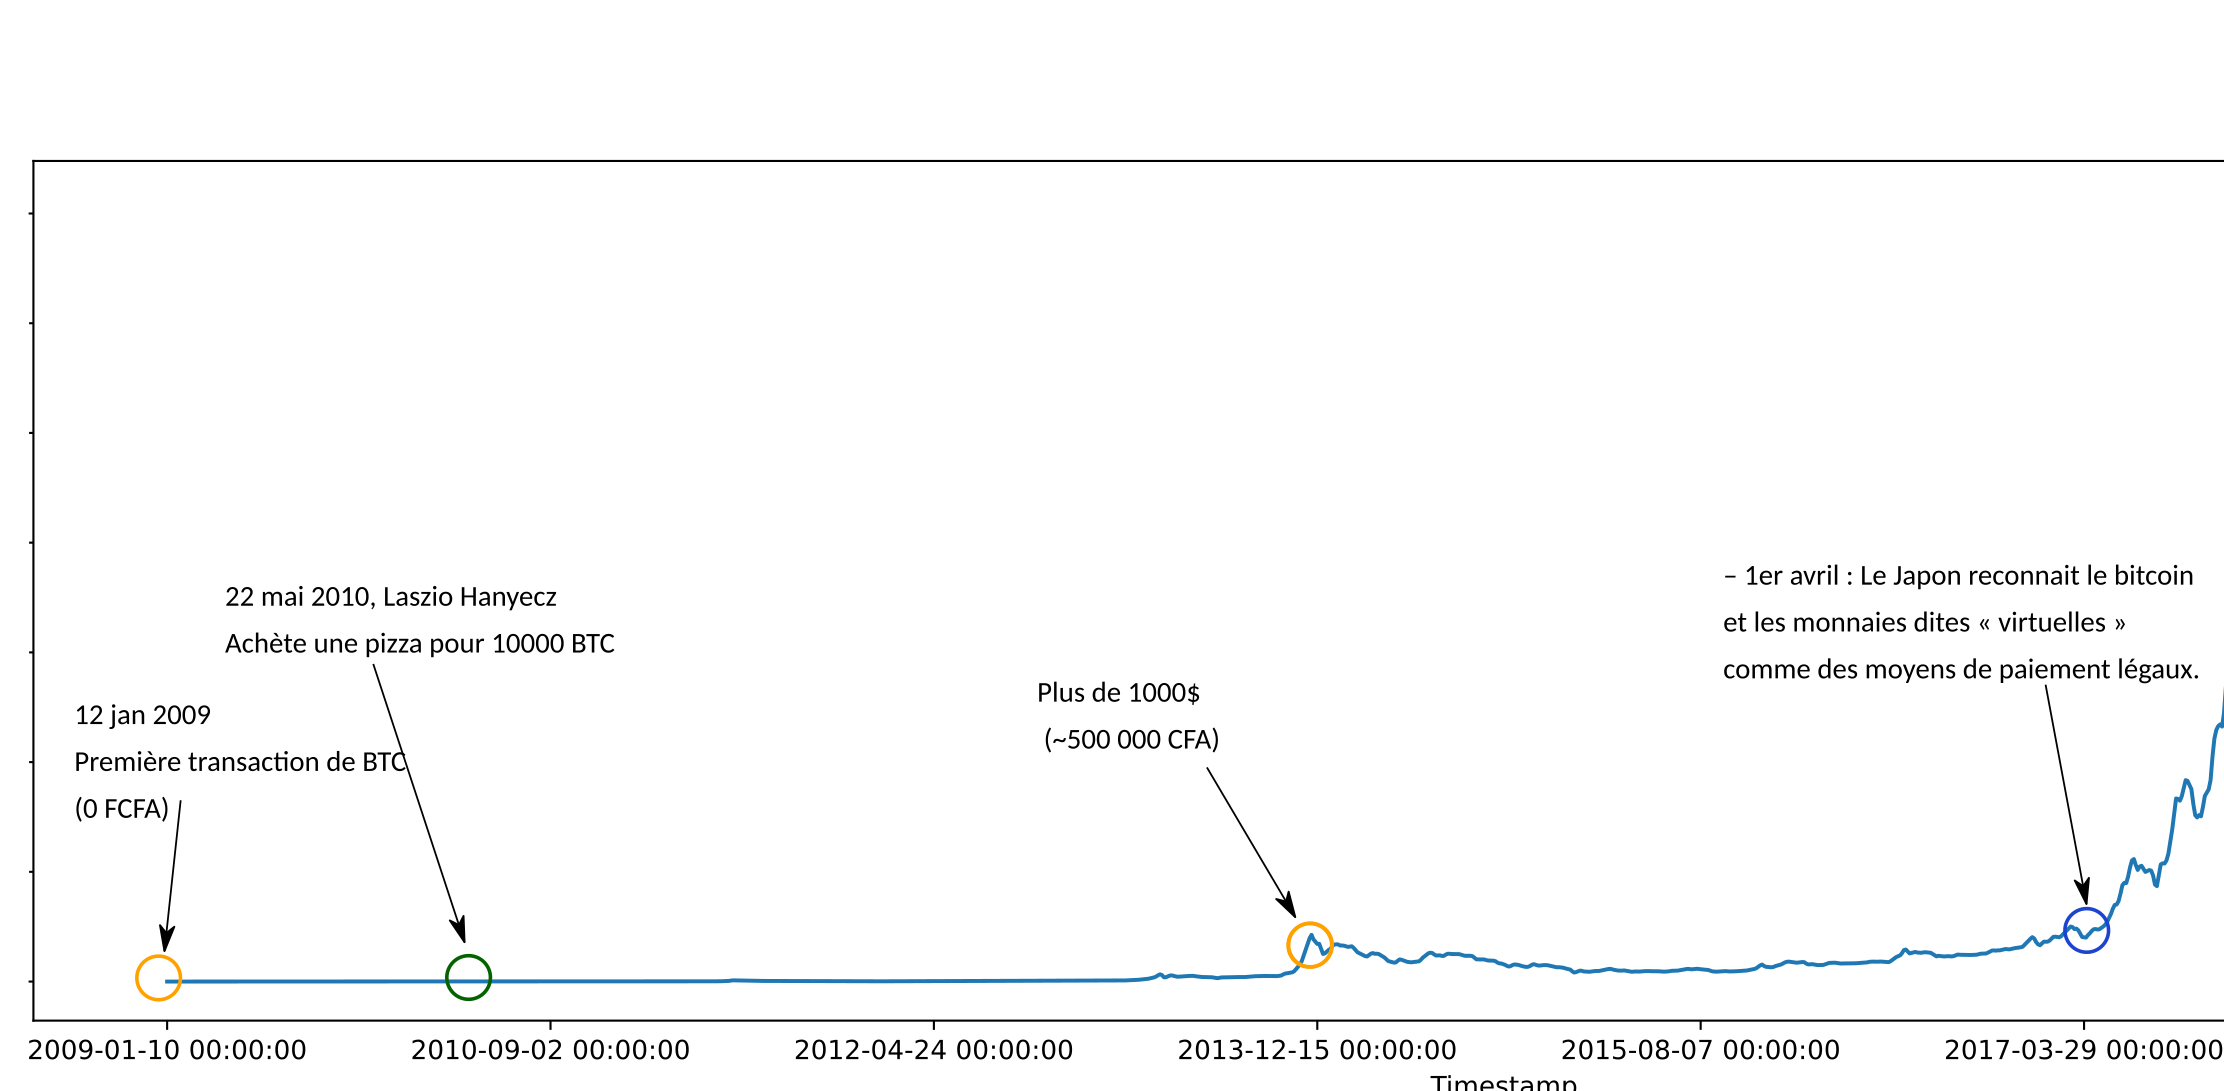
\includegraphics[width=1\textwidth]{./Pictures/Timeline/30hal_finney.png}
\end{center}
\end{block}

\begin{block}{}
\begin{center}
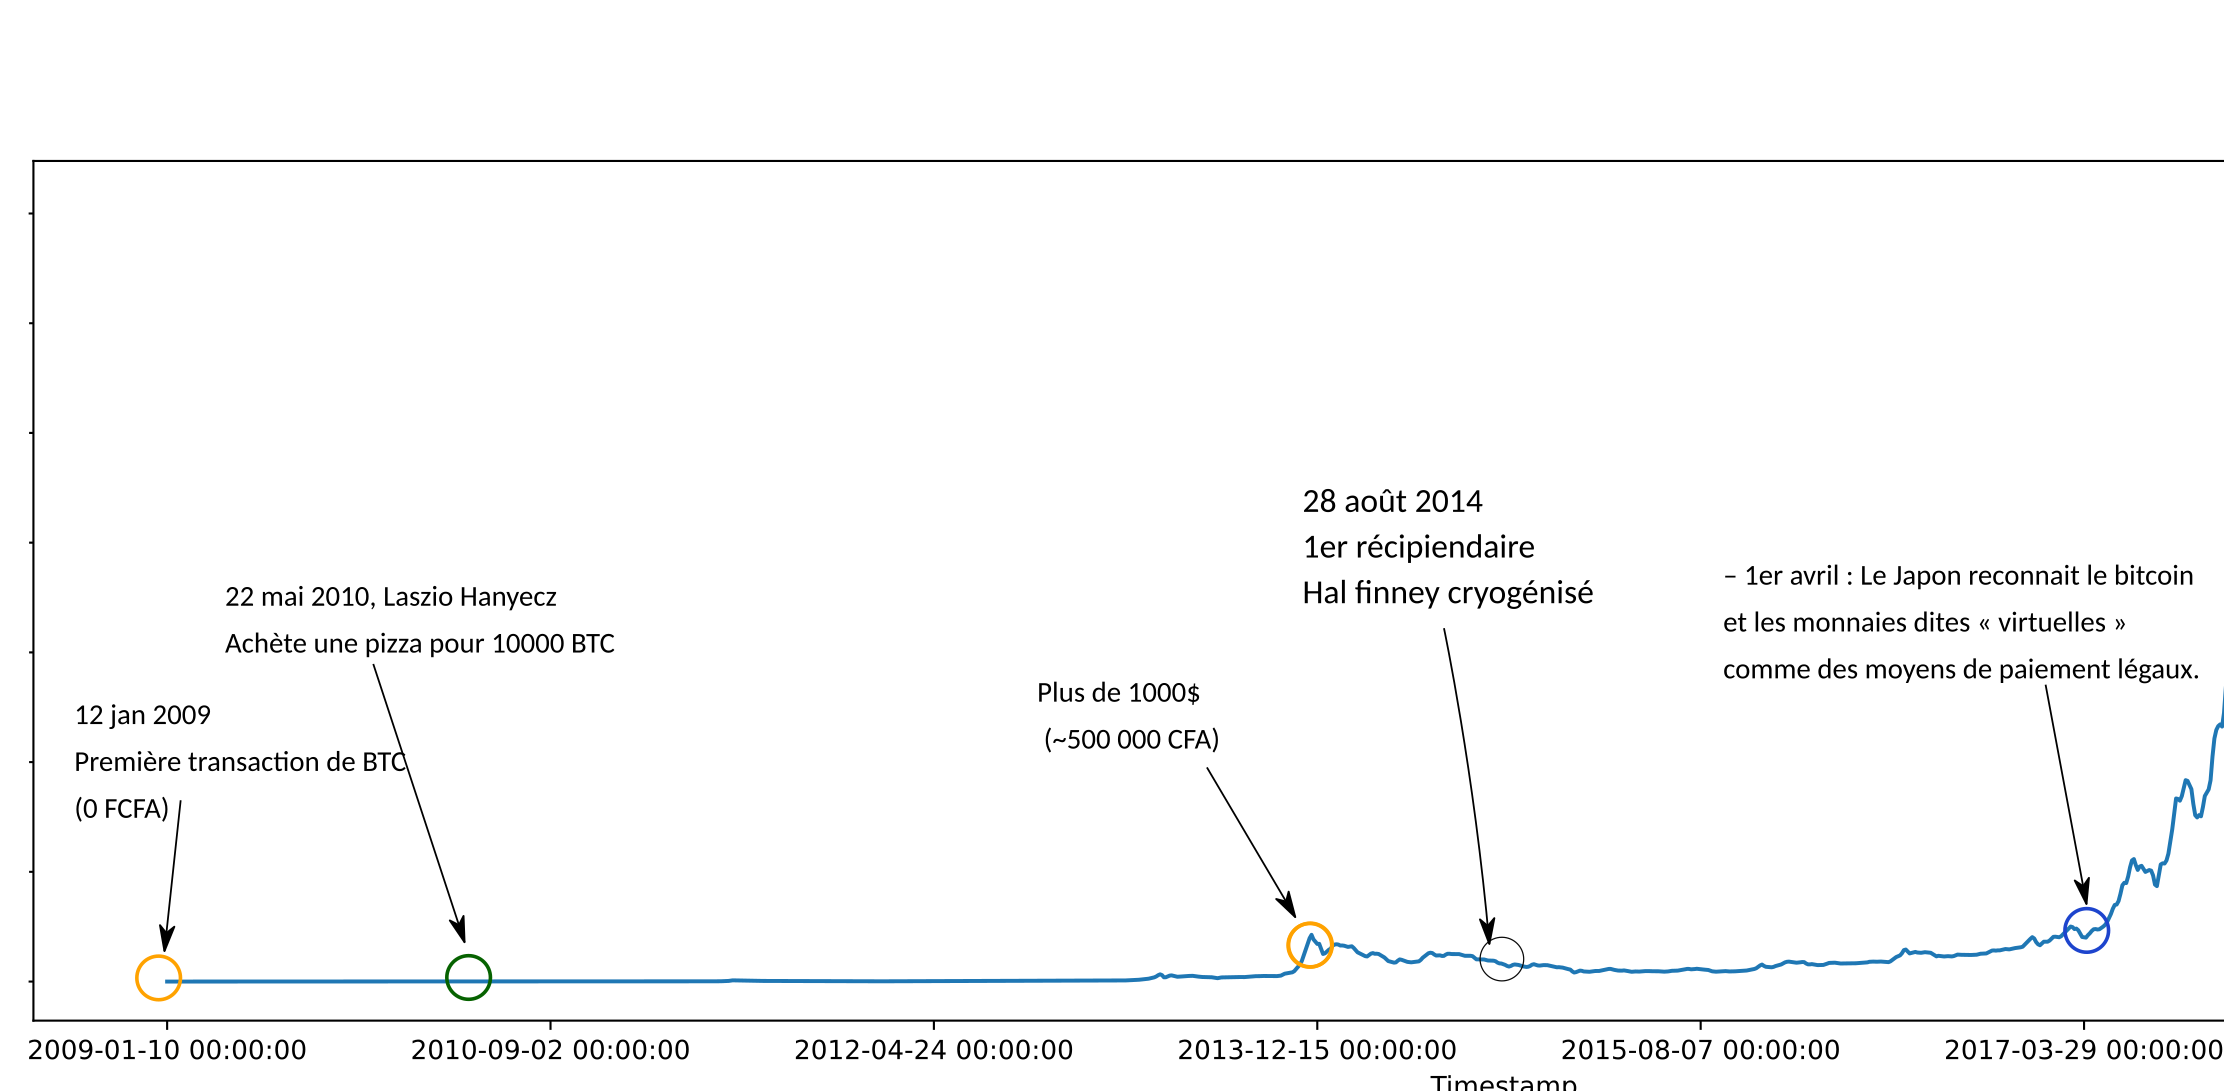
\includegraphics[width=1\textwidth]{./Pictures/Timeline/31hal_finney.png}
\end{center}
\end{block}

\begin{block}{}
\begin{center}
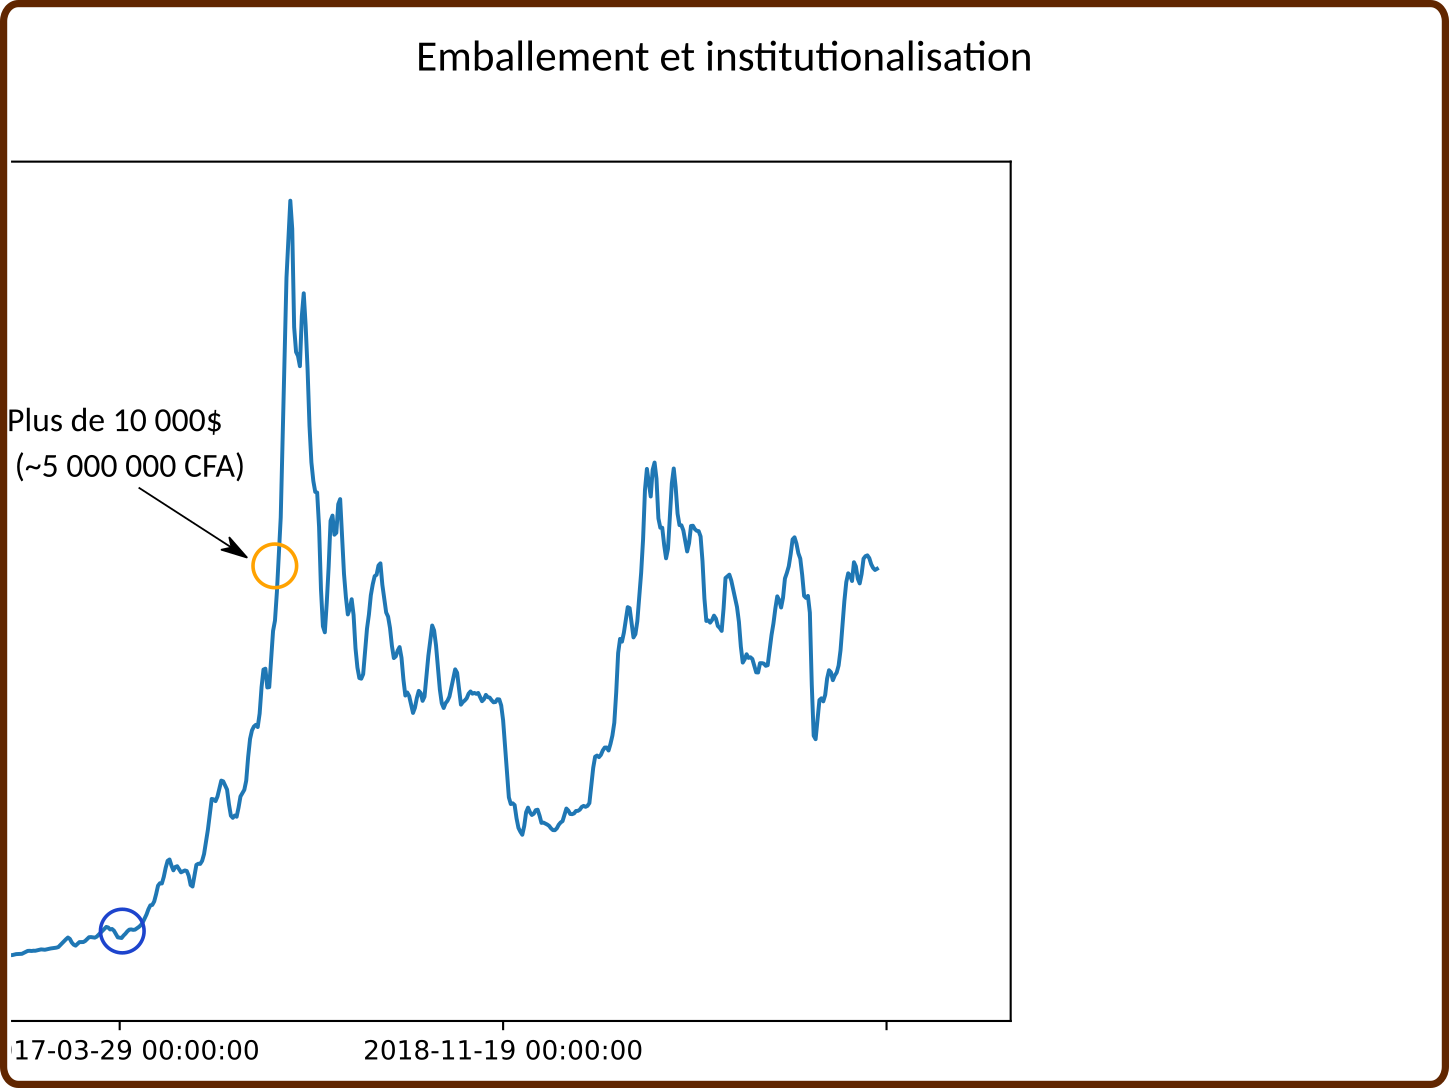
\includegraphics[width=.95\textwidth]{./Pictures/Timeline/40emballement.png}
\end{center}
\end{block}

\begin{block}{}
\begin{center}
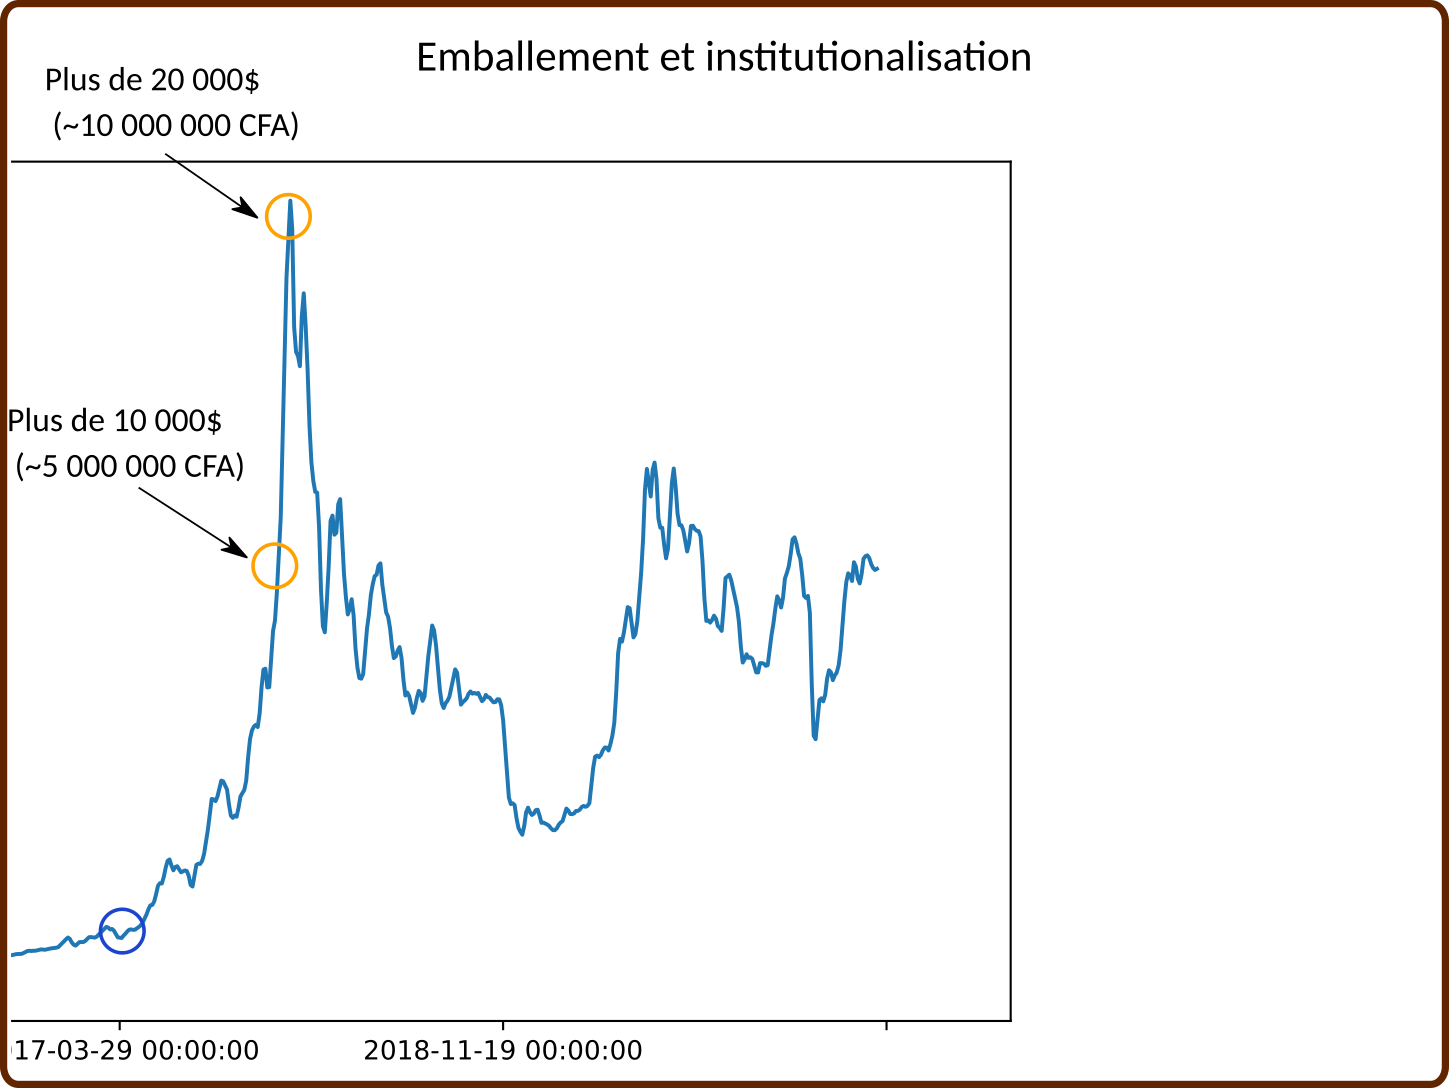
\includegraphics[width=.95\textwidth]{./Pictures/Timeline/41emballement_20000.png}
\end{center}
\end{block}

\begin{block}{}
\begin{center}
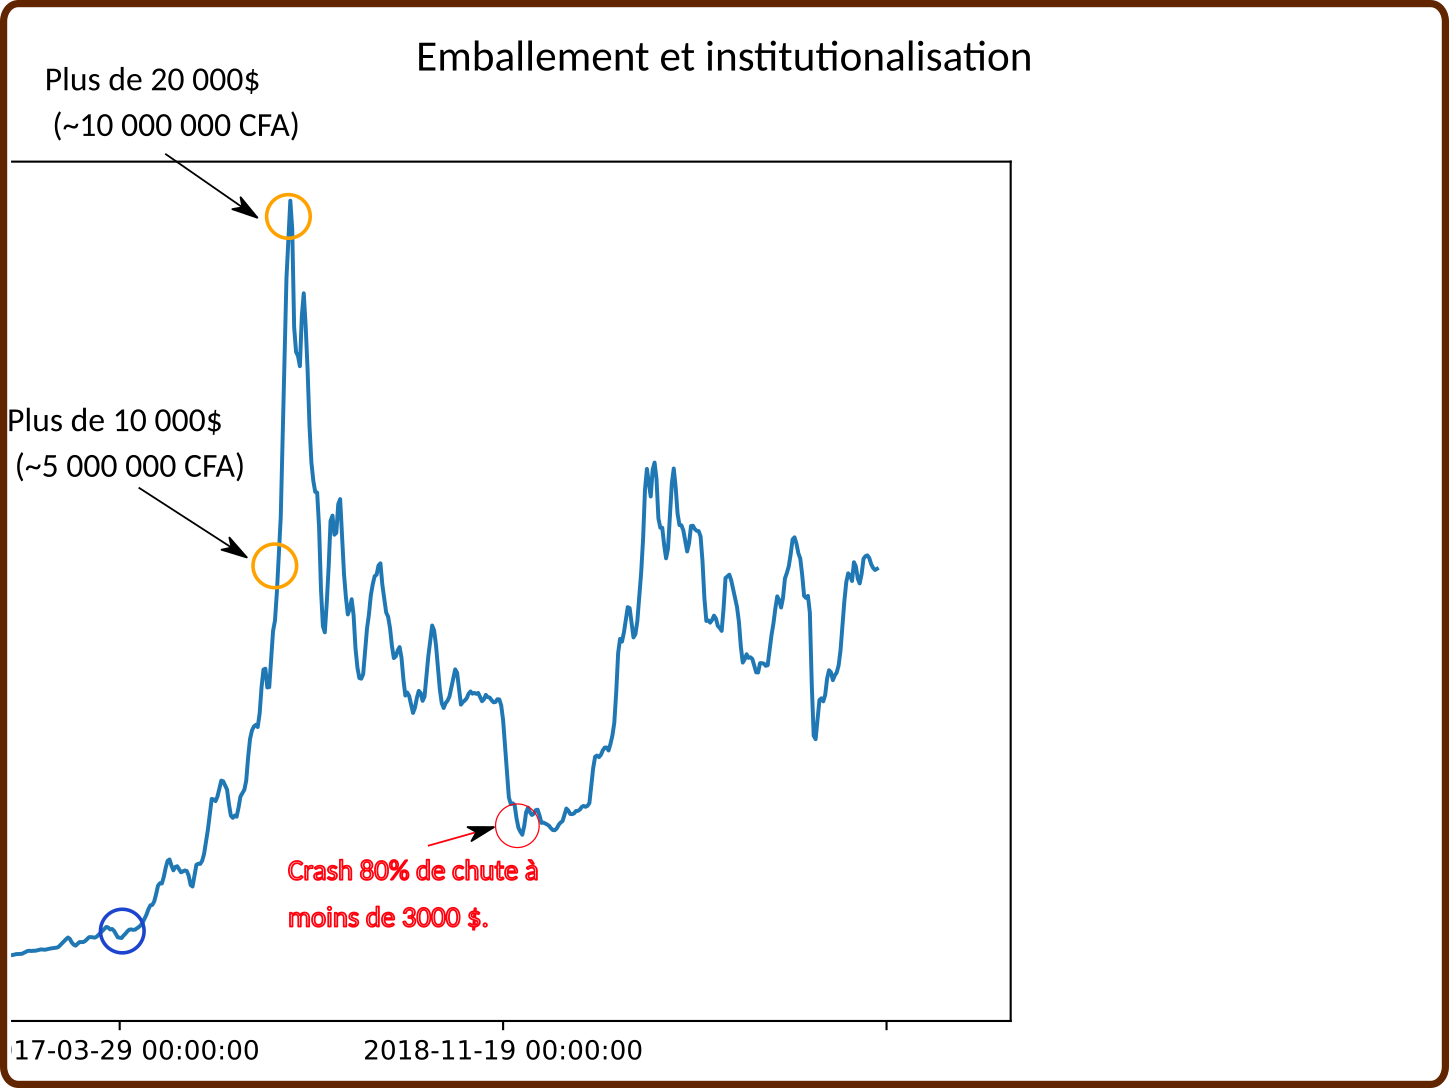
\includegraphics[width=.95\textwidth]{./Pictures/Timeline/42emballement_crash3.png}
\end{center}
\end{block}

\begin{block}{}
\begin{center}
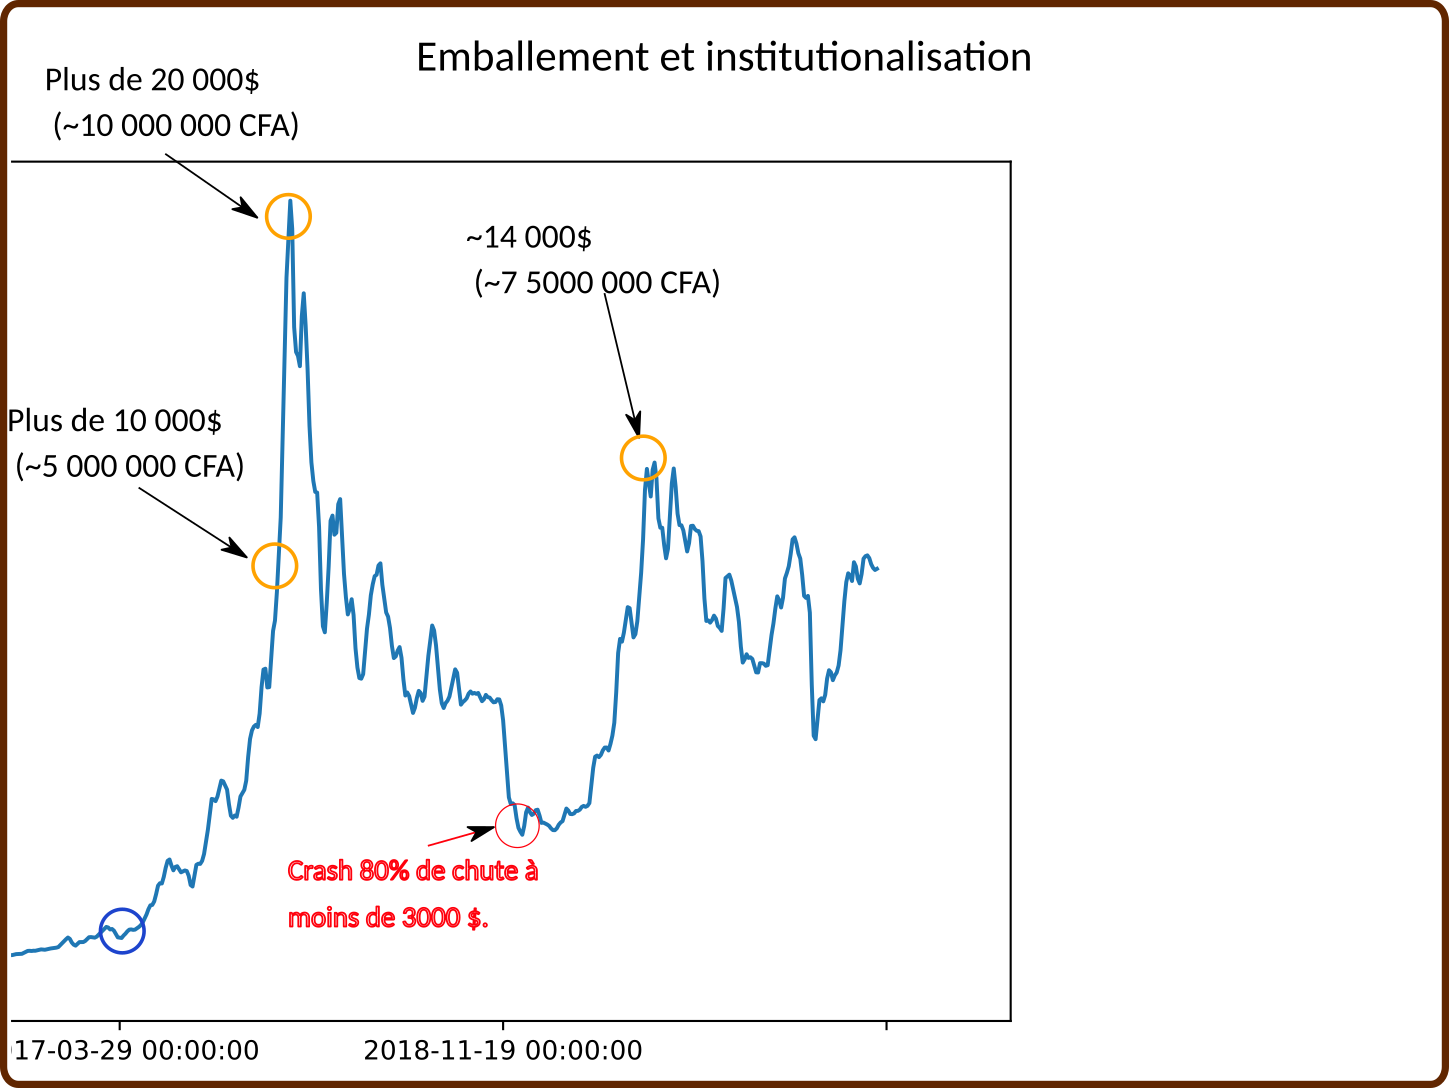
\includegraphics[width=.95\textwidth]{./Pictures/Timeline/43emballement_rebond.png}
\end{center}
\end{block}

\begin{block}{}
\begin{center}
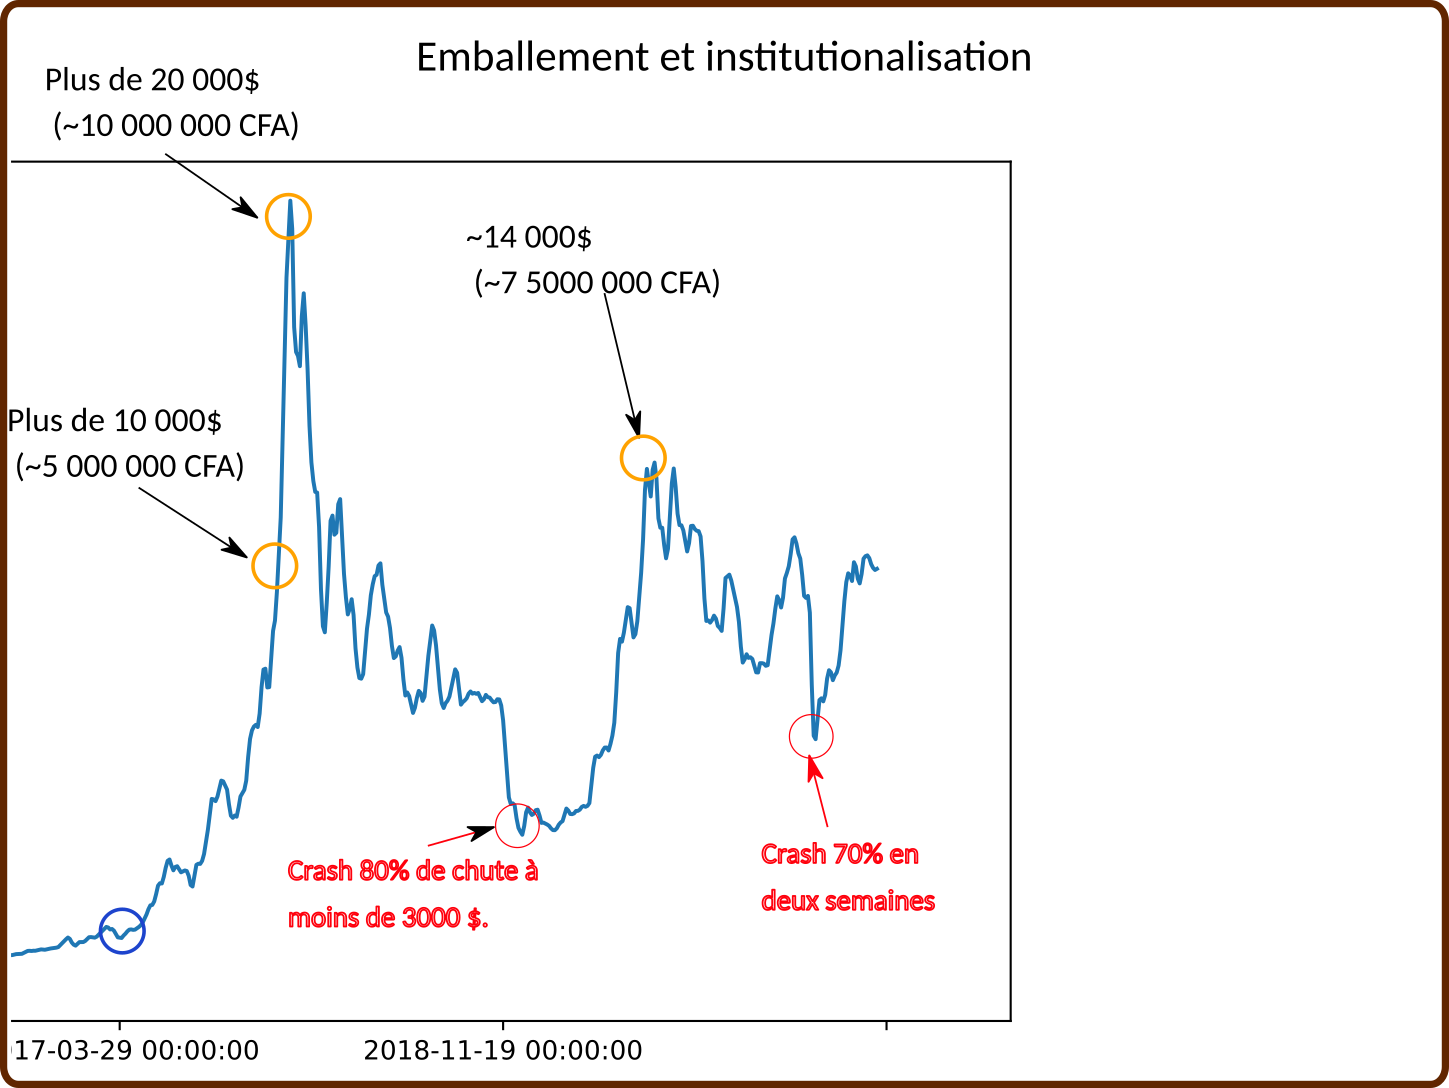
\includegraphics[width=.95\textwidth]{./Pictures/Timeline/44emballement_crash4.png}
\end{center}
\end{block}

\begin{block}{}
\begin{center}
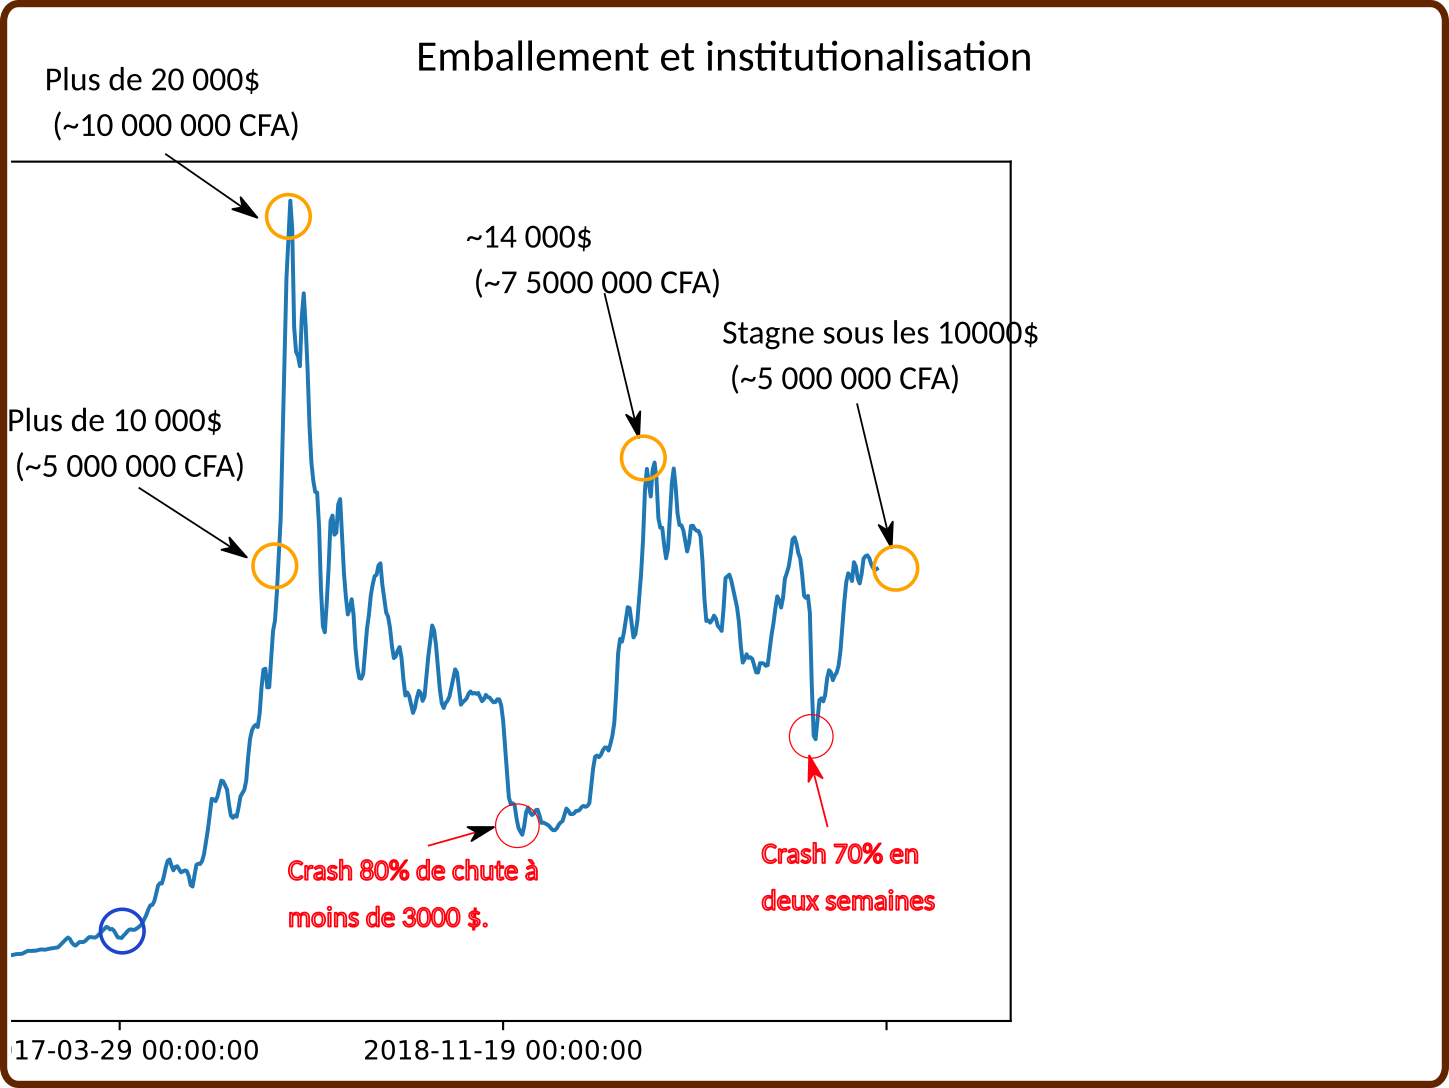
\includegraphics[width=.95\textwidth]{./Pictures/Timeline/45emballement_aujourdhui.png}
\end{center}
\end{block}

\begin{block}{}
\begin{center}
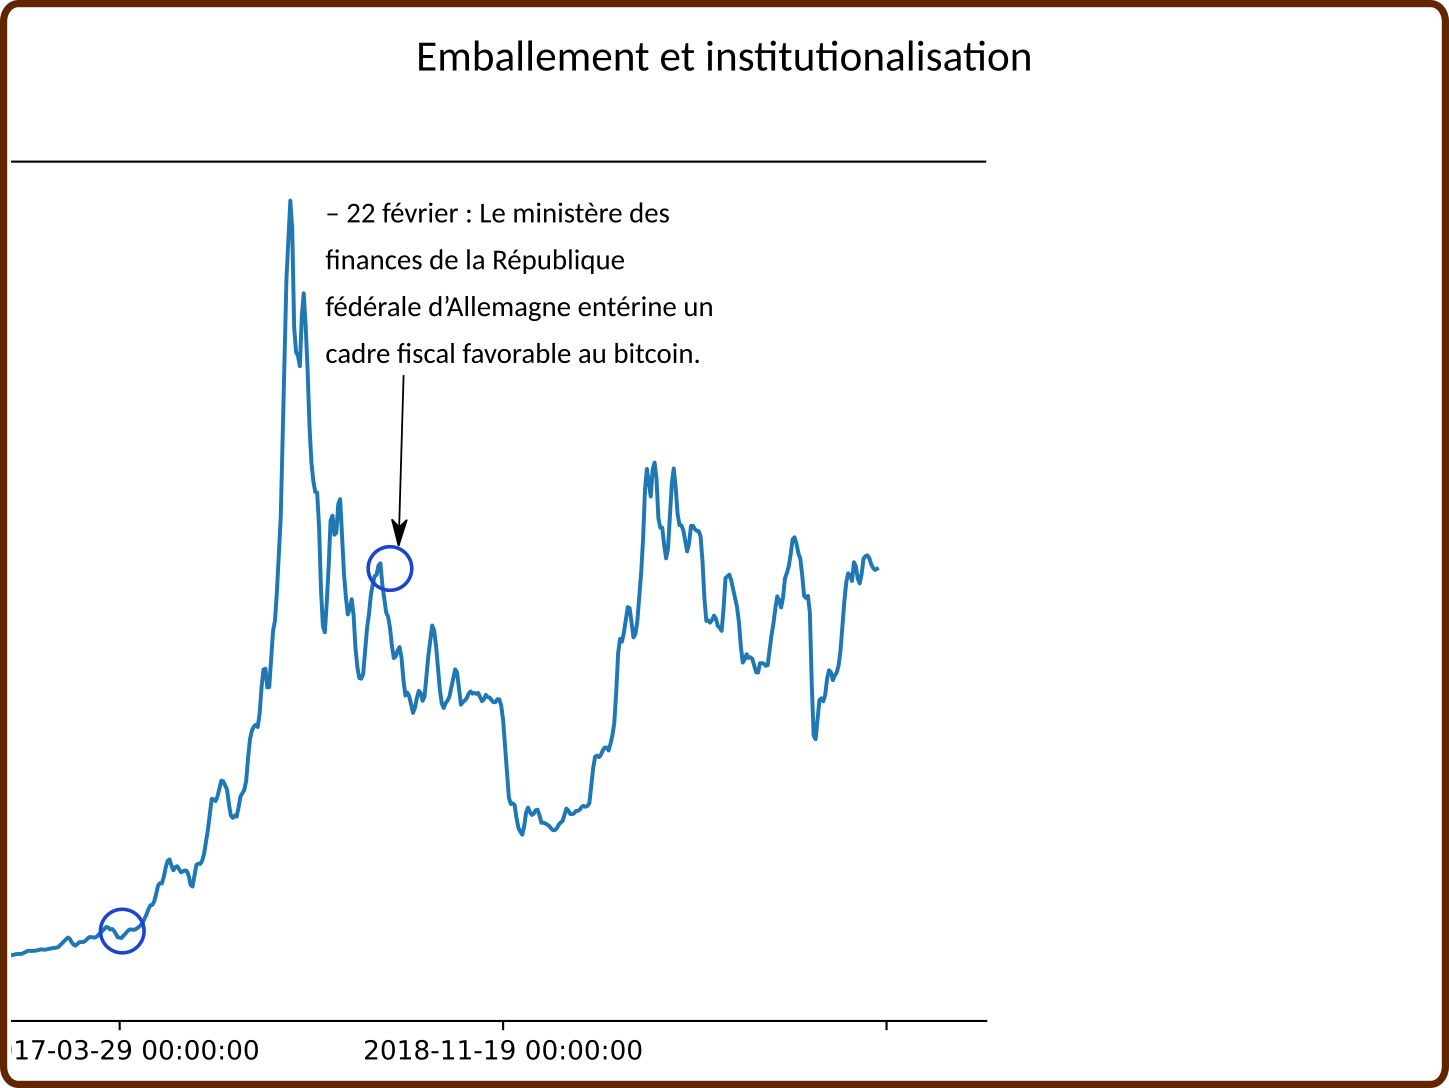
\includegraphics[width=.95\textwidth]{./Pictures/Timeline/50emballement_banque.png}
\end{center}
\end{block}

\begin{block}{}
\begin{center}
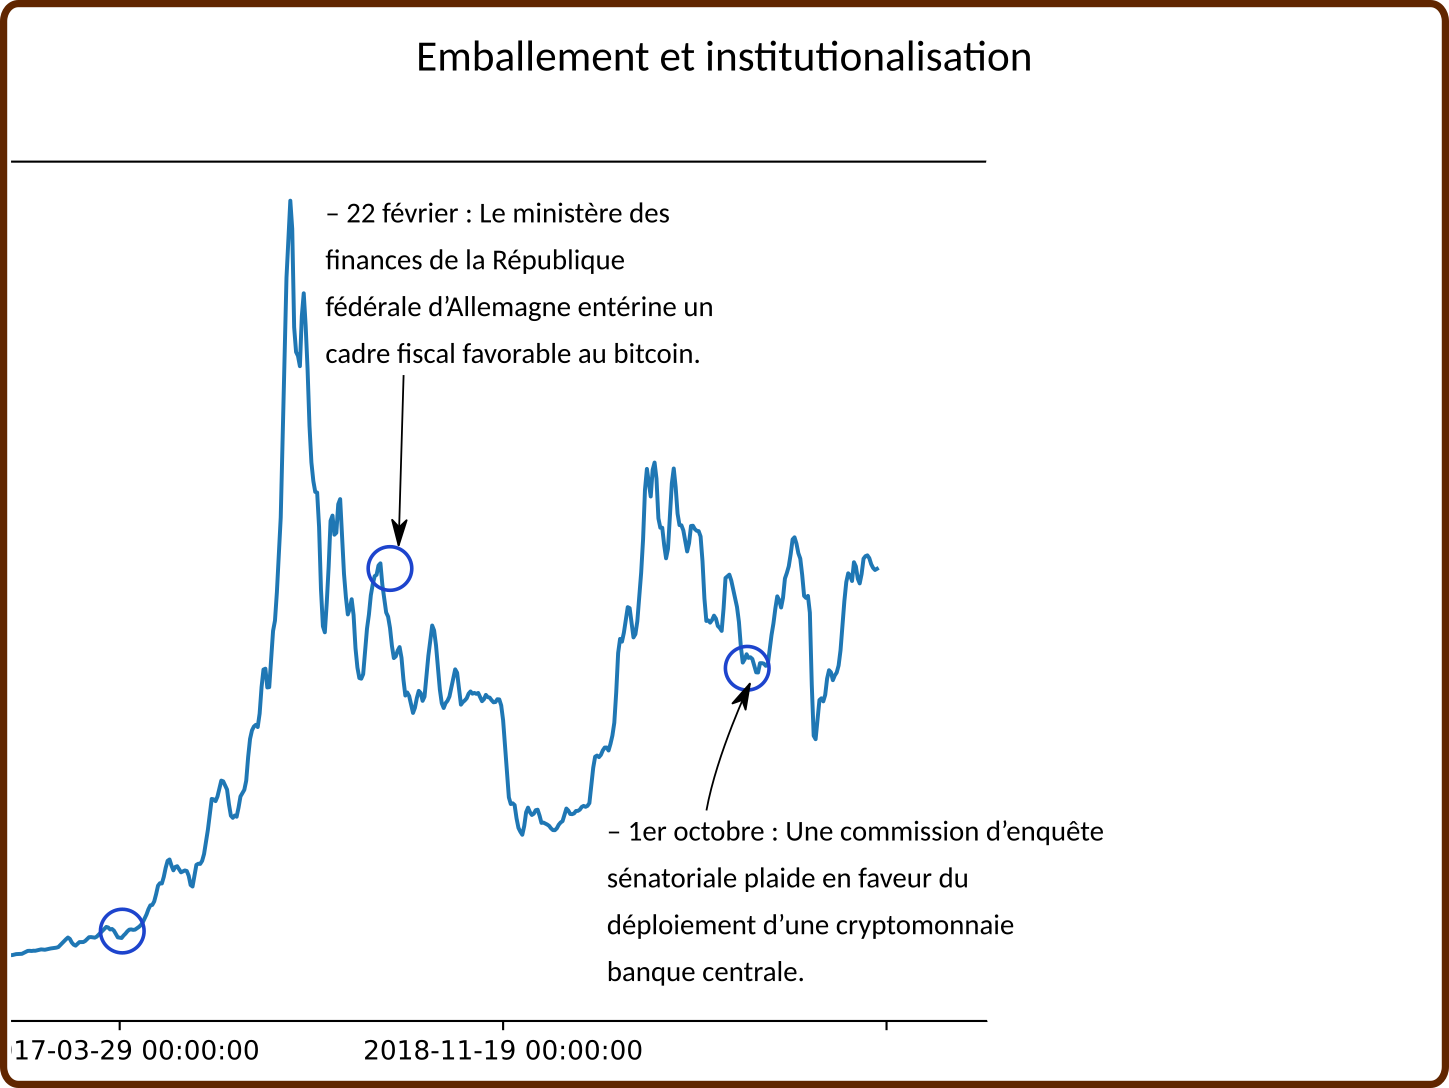
\includegraphics[width=.95\textwidth]{./Pictures/Timeline/51emballement_senat.png}
\end{center}
\end{block}

\begin{block}{}
\begin{center}
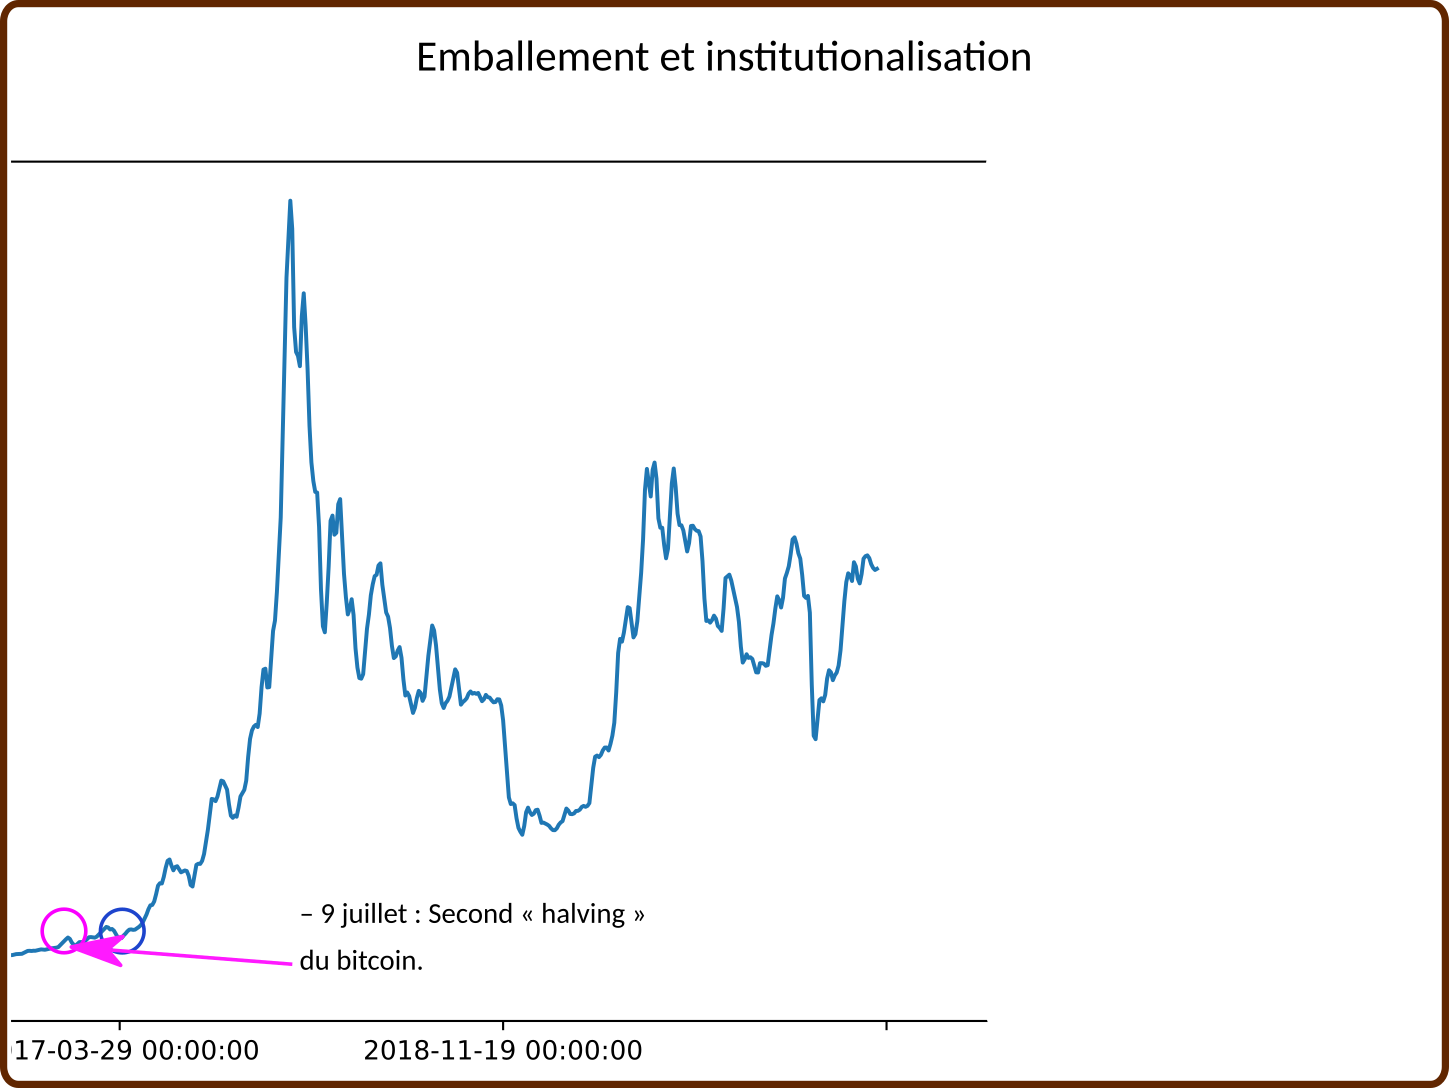
\includegraphics[width=.95\textwidth]{./Pictures/Timeline/60emballement_halving.png}
\end{center}
\end{block}

\begin{block}{}
\begin{center}
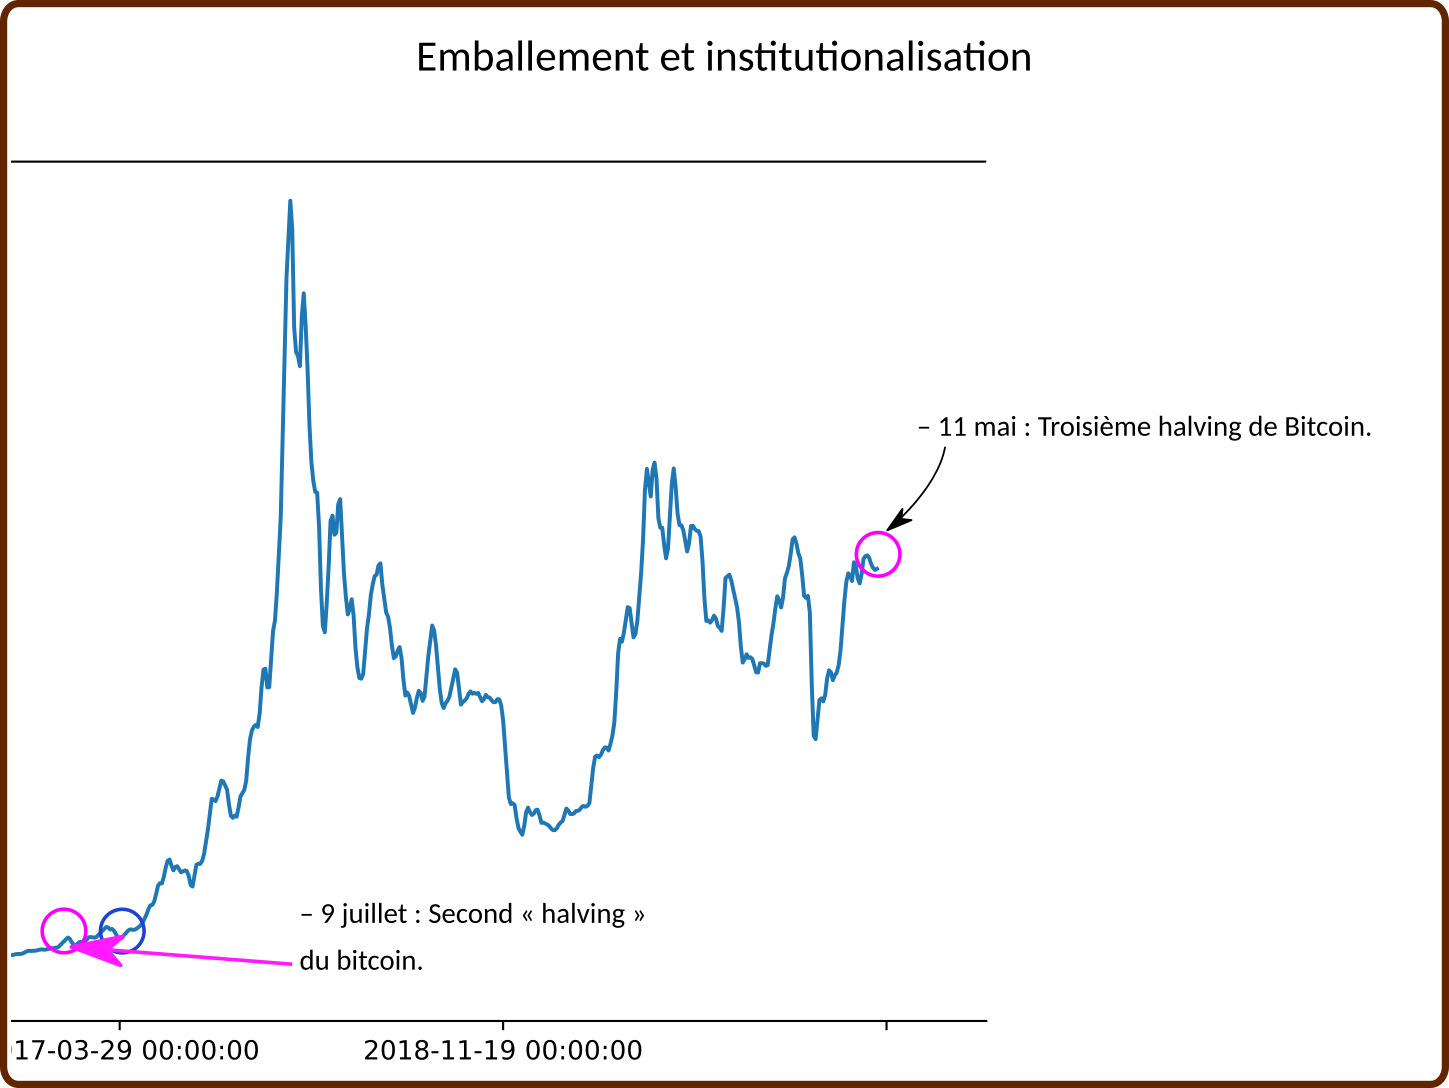
\includegraphics[width=.95\textwidth]{./Pictures/Timeline/61emballement_halving2.png}
\end{center}
\end{block}

\begin{block}{}
\begin{center}
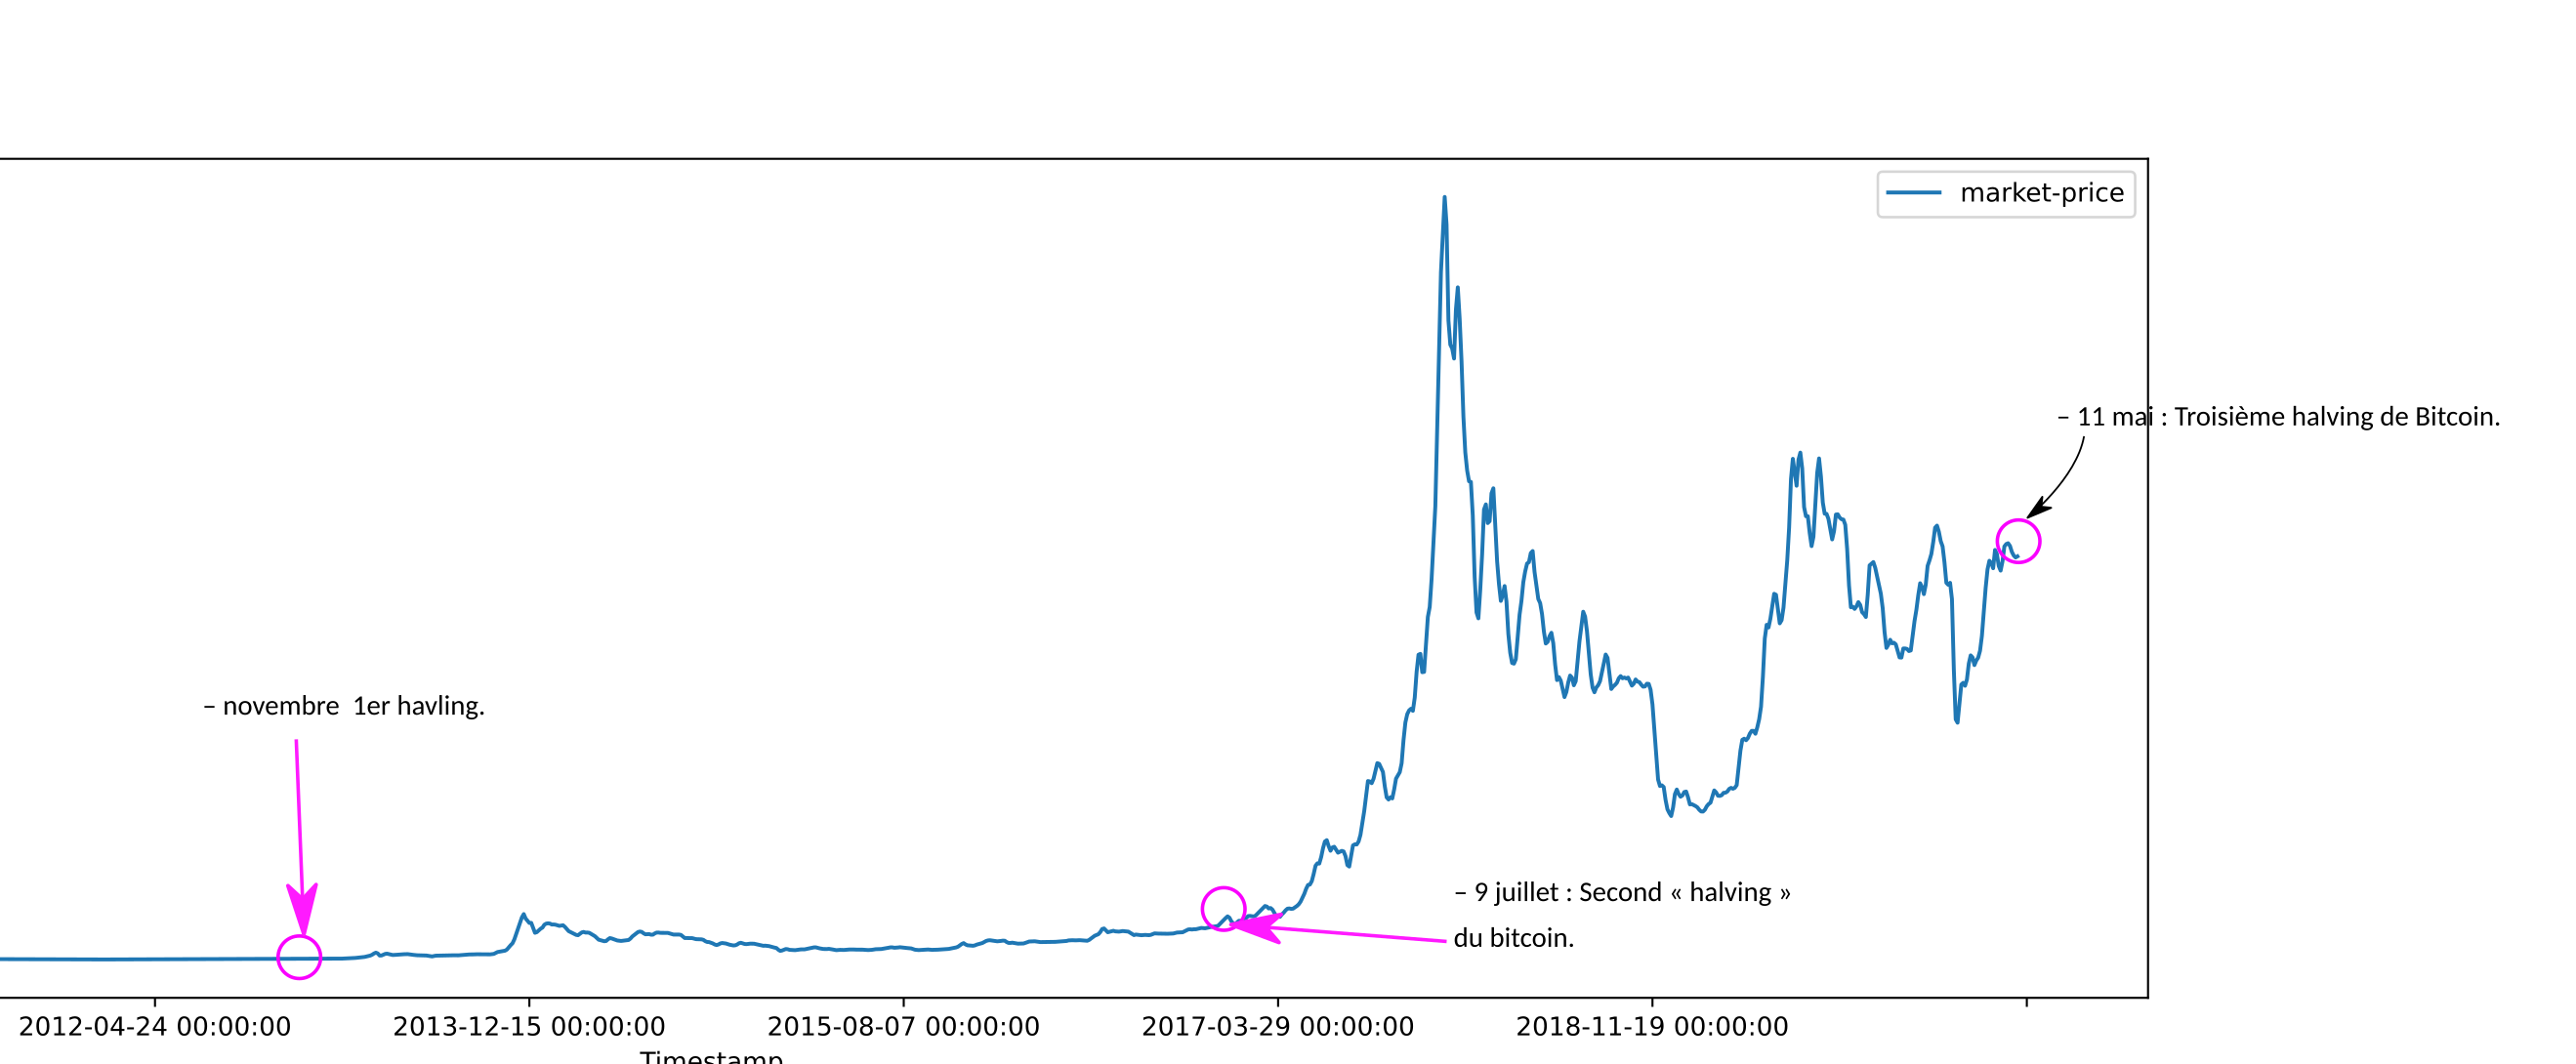
\includegraphics[width=1.05\textwidth]{./Pictures/Timeline/62emballement_halvings.png}
\end{center}
\end{block}

\begin{block}{}
\begin{center}
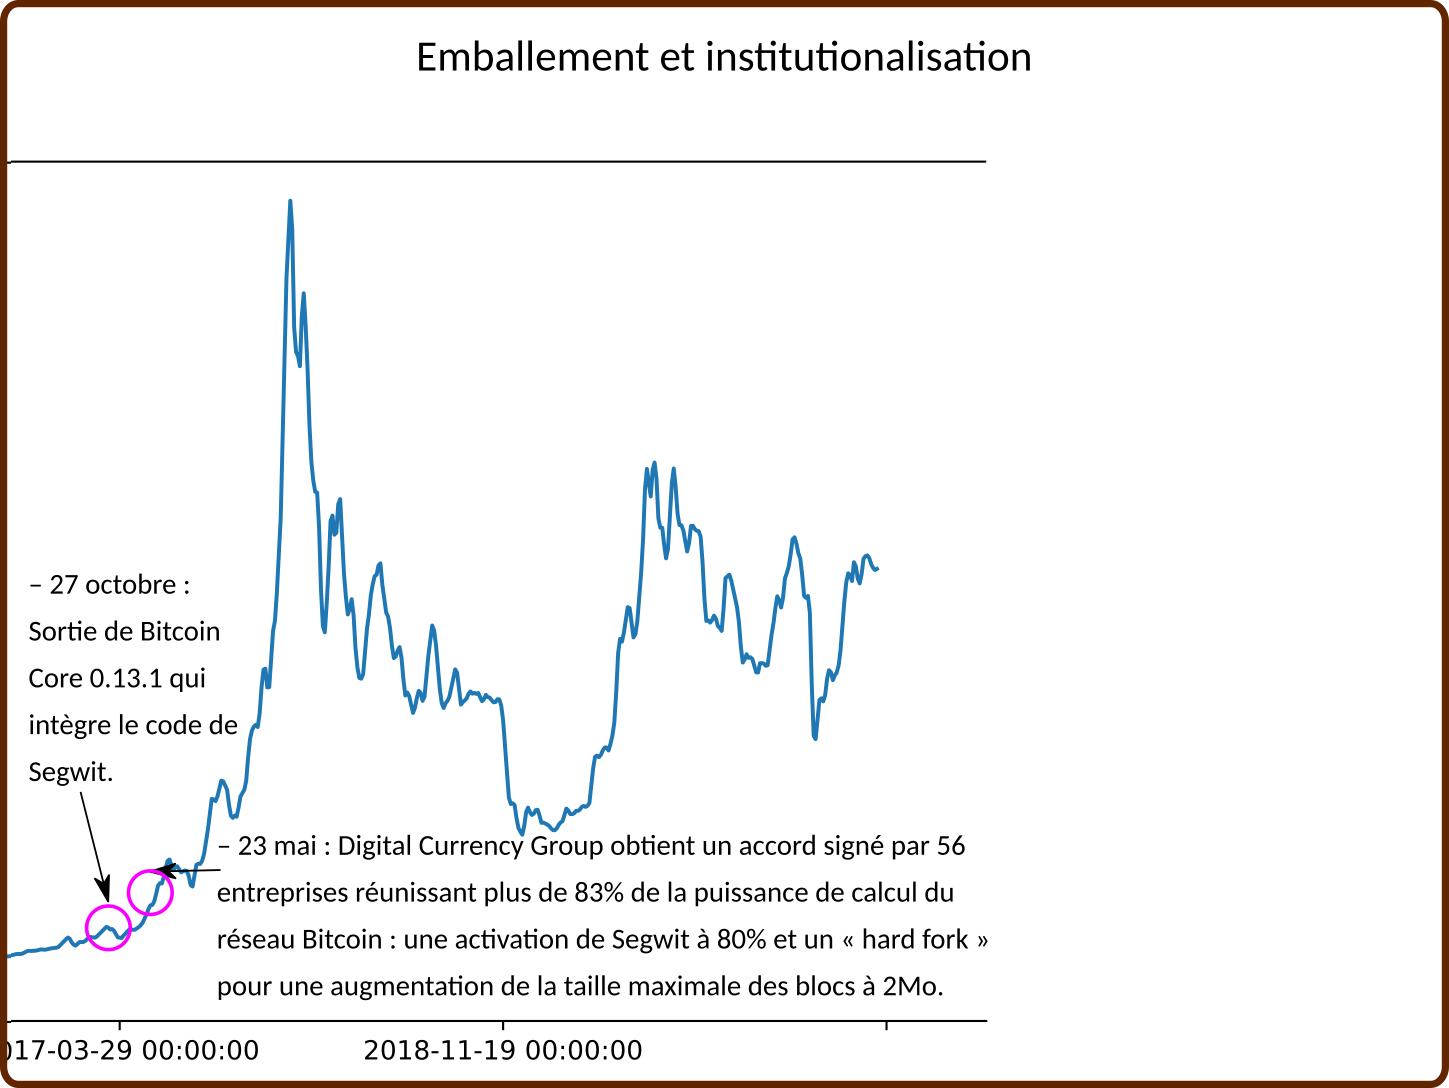
\includegraphics[width=.95\textwidth]{./Pictures/Timeline/70emballement_segwit.png}
\end{center}
\end{block}

\begin{block}{}
\begin{center}
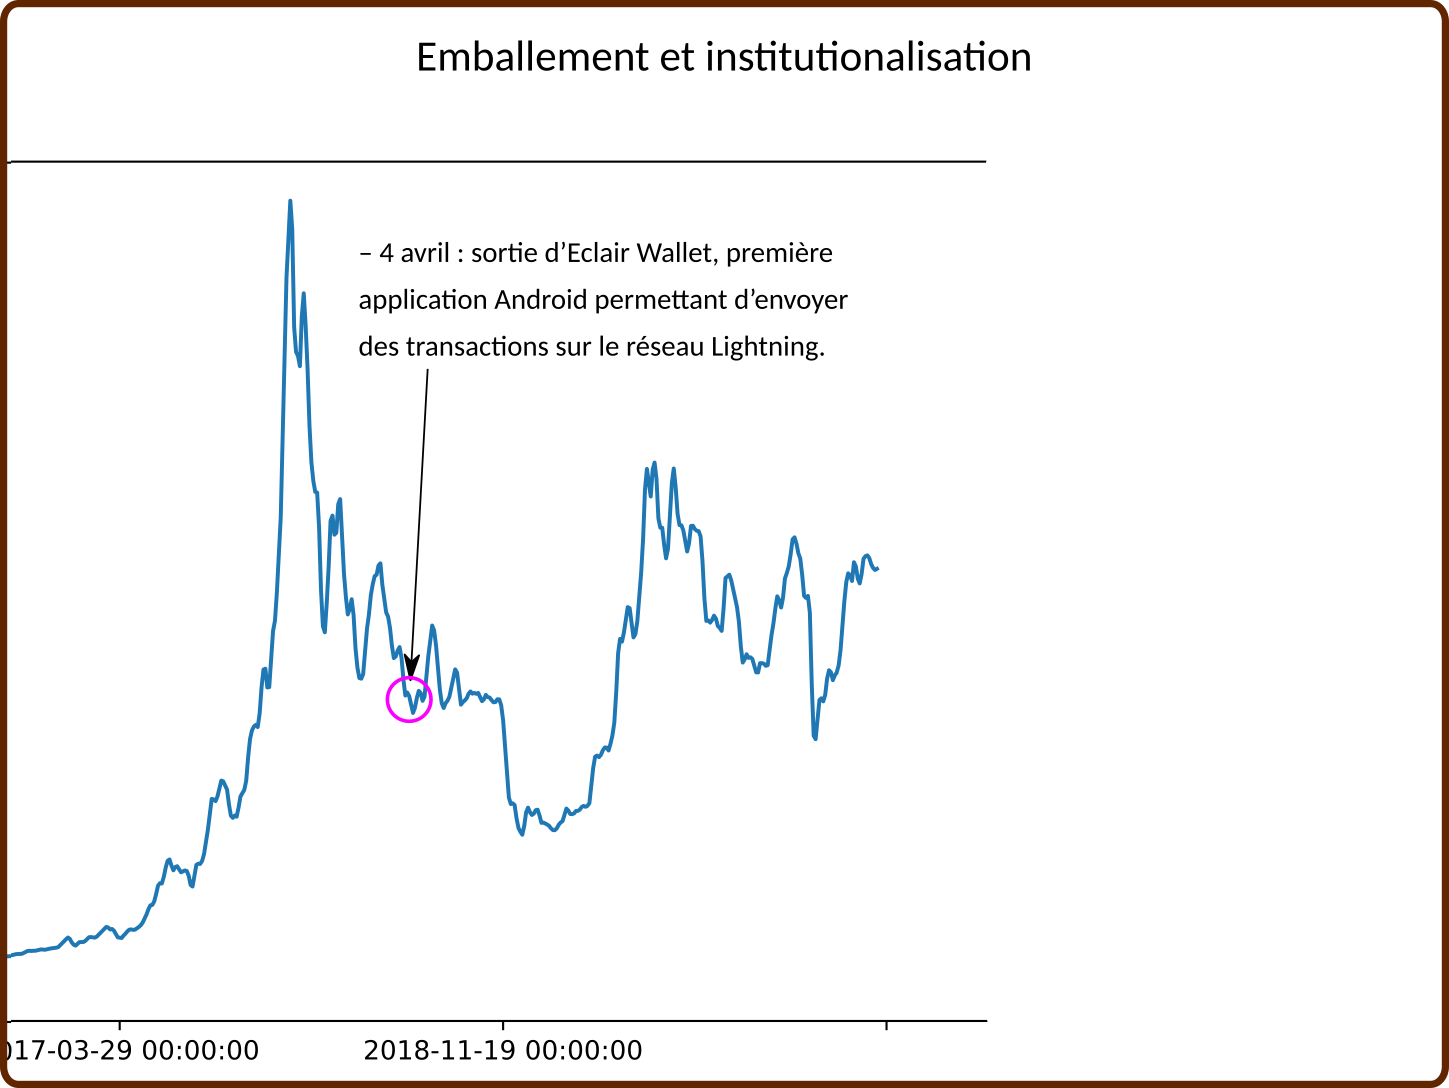
\includegraphics[width=.95\textwidth]{./Pictures/Timeline/71emballement_lightning.png}
\end{center}
\end{block}

\begin{block}{}
\begin{center}
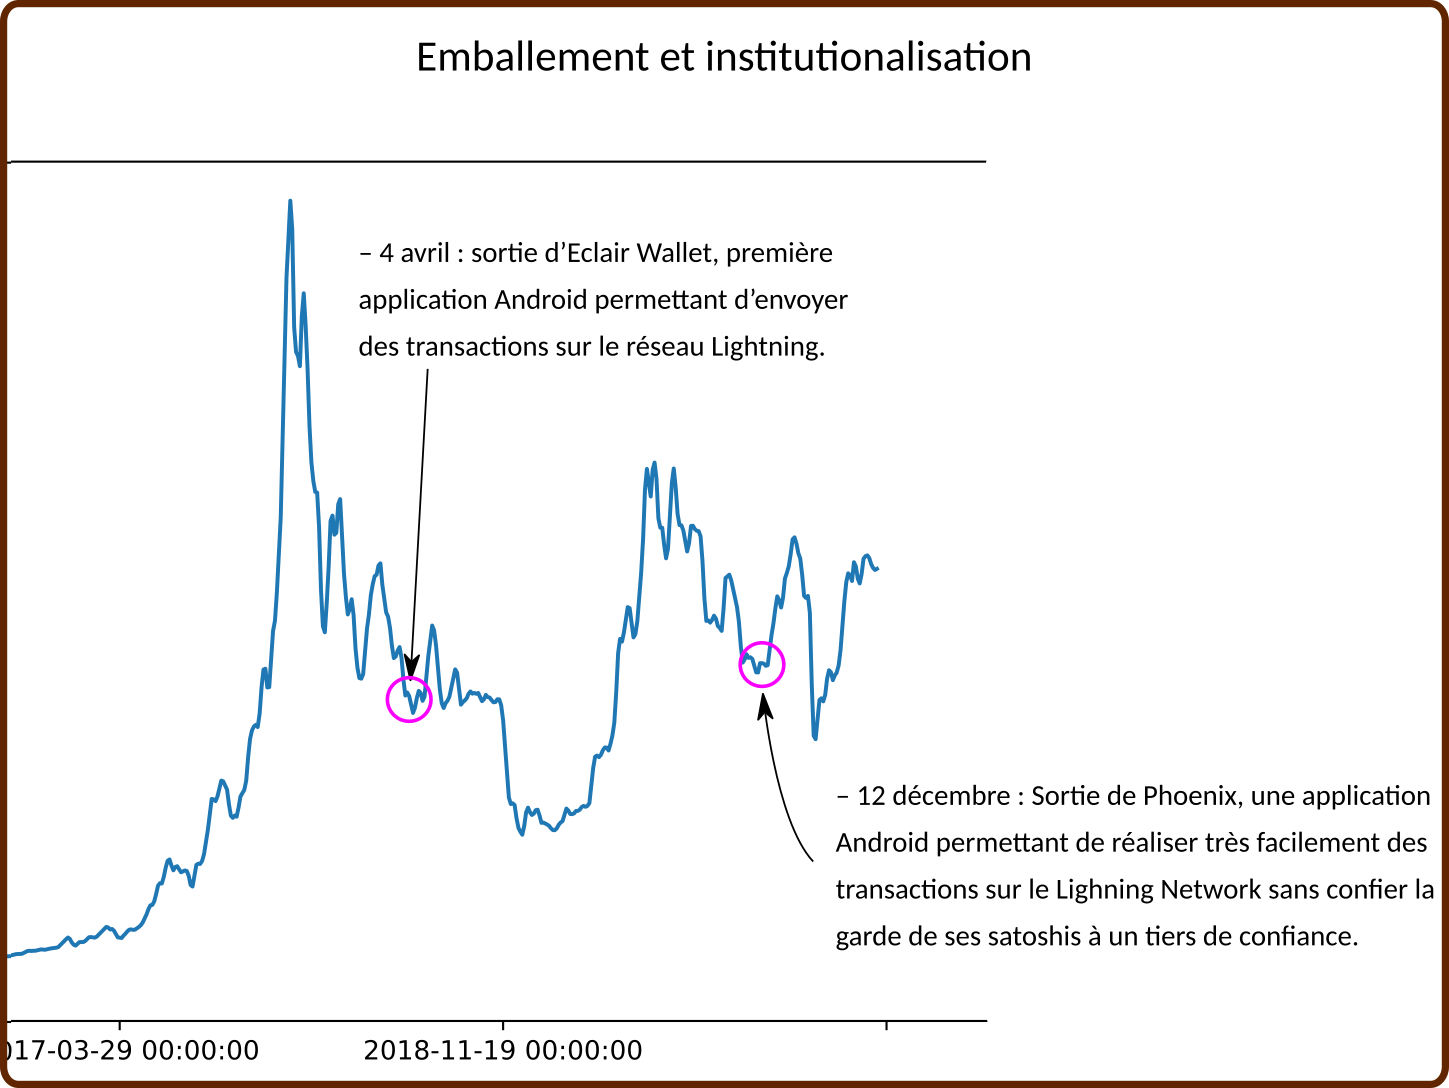
\includegraphics[width=.95\textwidth]{./Pictures/Timeline/72emballement_phoenix.png}
\end{center}
\end{block}

\begin{block}{}
\begin{center}
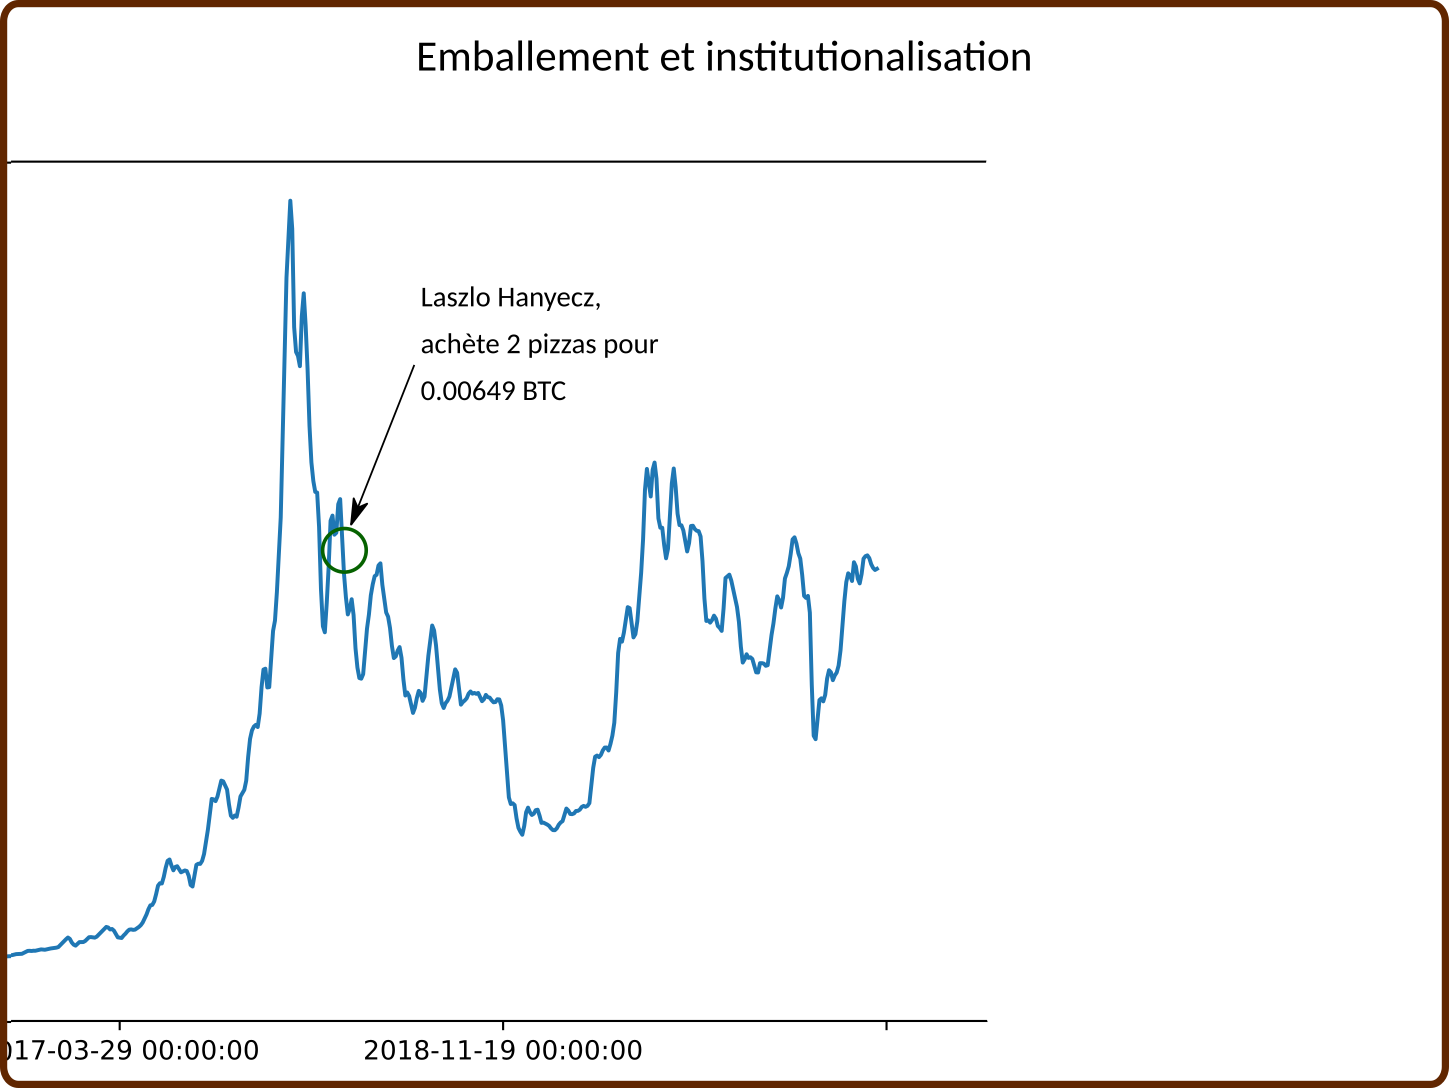
\includegraphics[width=.95\textwidth]{./Pictures/Timeline/80emballement_pizza.png}
\end{center}
\end{block}

\begin{block}{}
\begin{center}
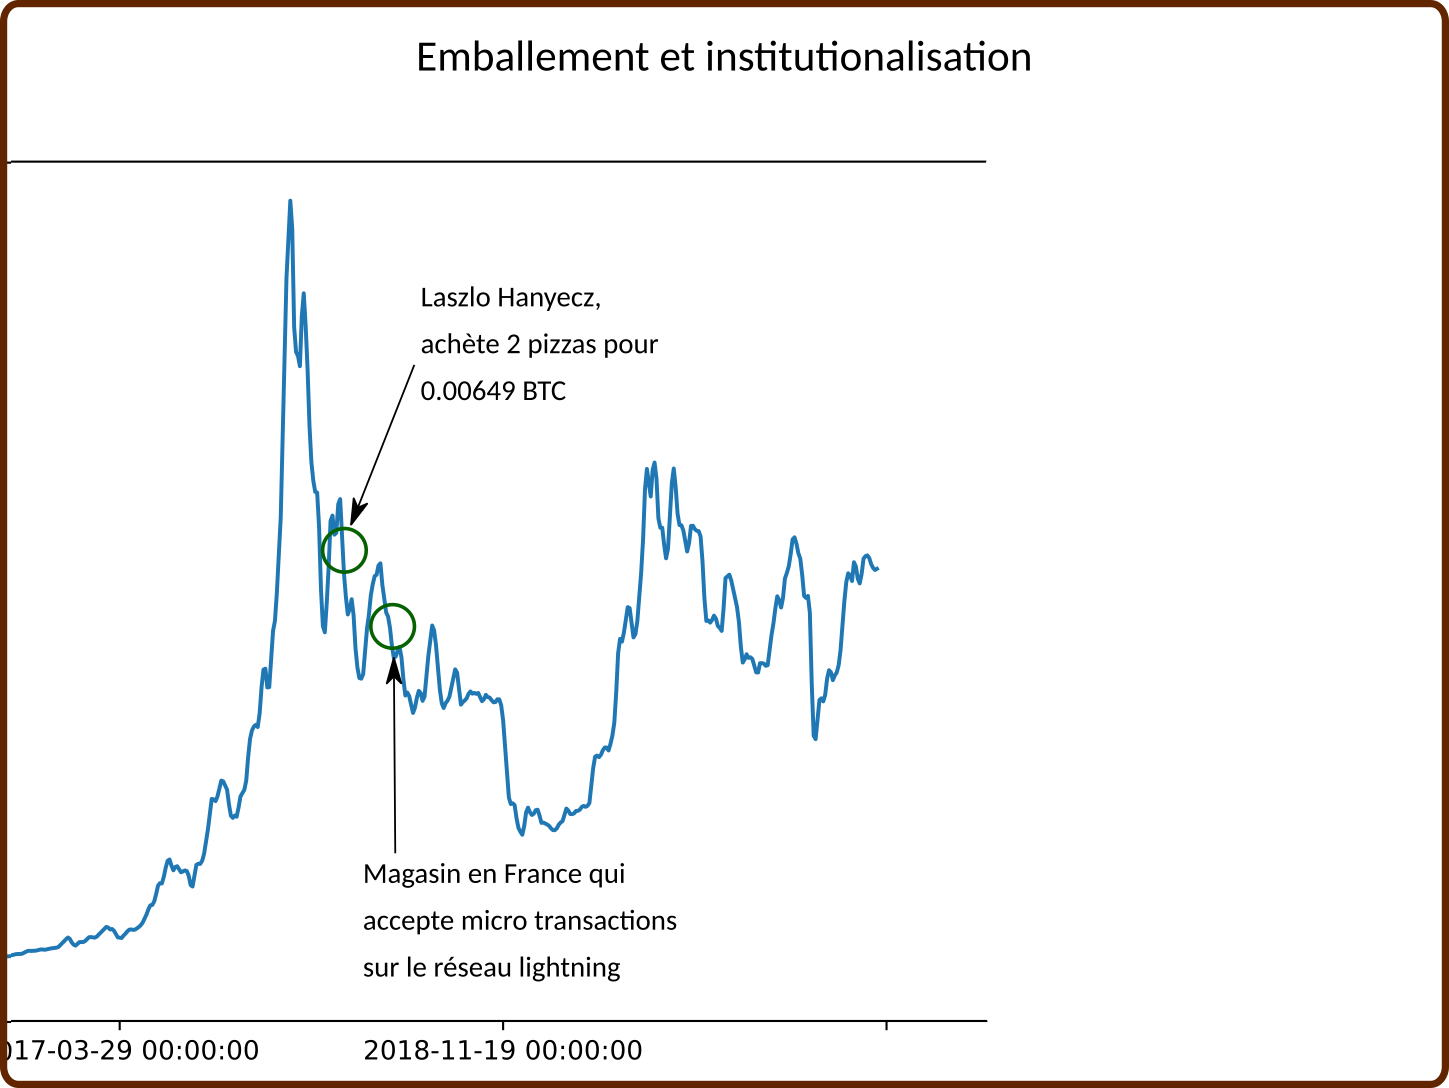
\includegraphics[width=.95\textwidth]{./Pictures/Timeline/81emballement_magasin.png}
\end{center}
\end{block}

\begin{block}{}
\begin{center}
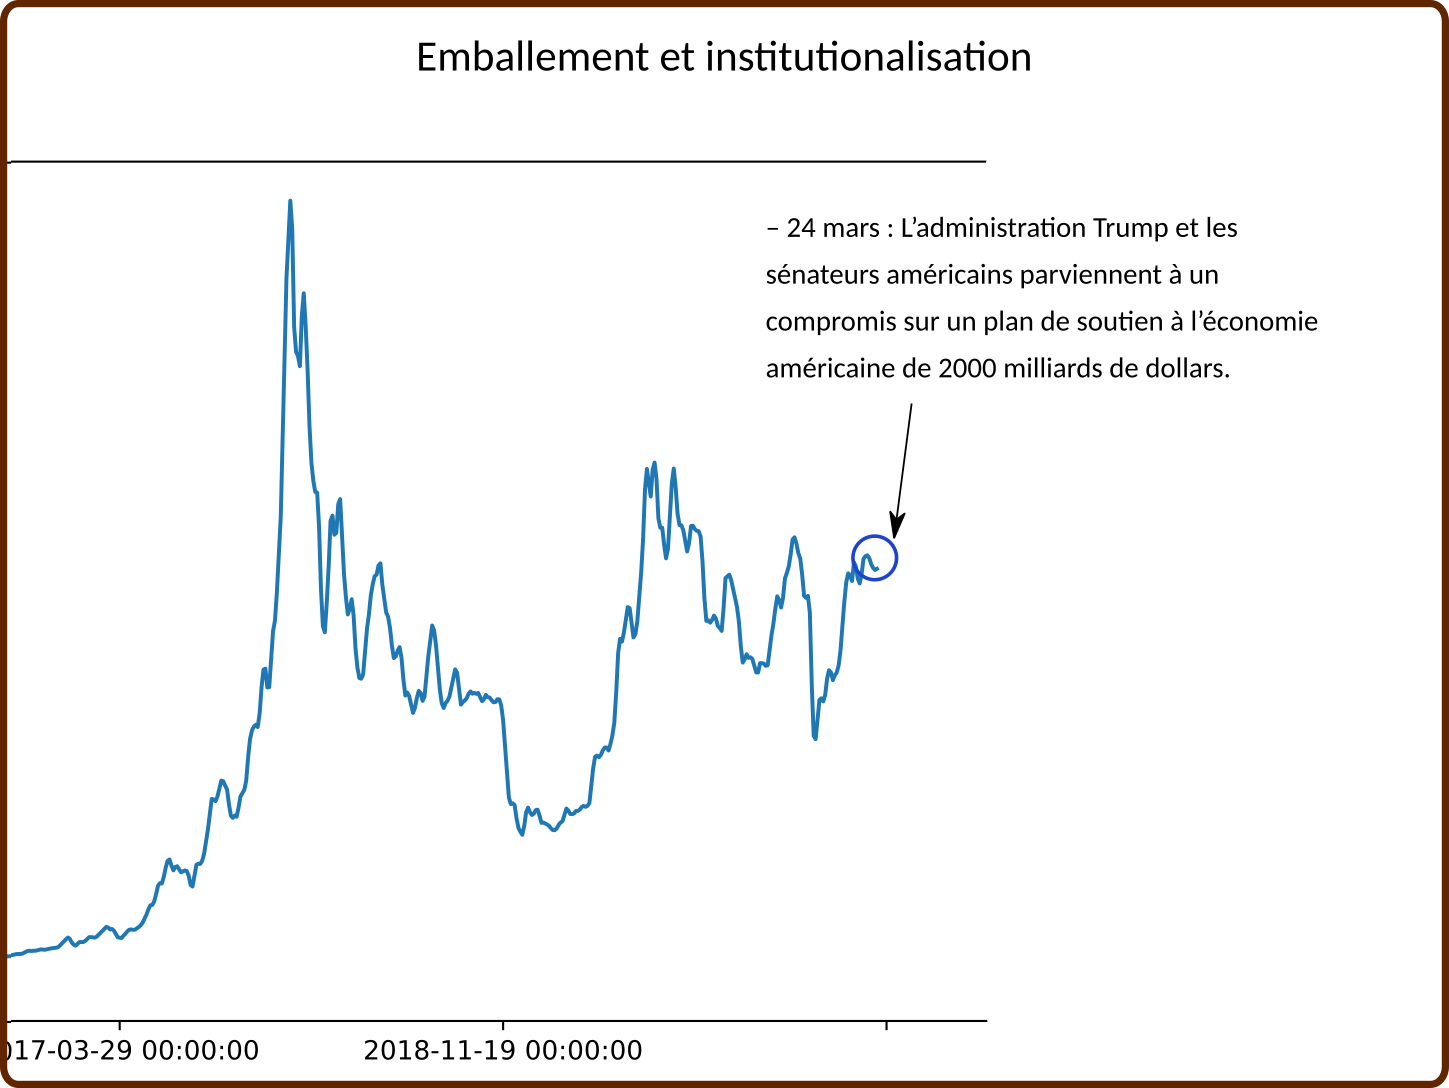
\includegraphics[width=.95\textwidth]{./Pictures/Timeline/90emballement_trump.png}
\end{center}
\end{block}

\begin{block}{et aujourd'hui ?}
\href{https://www.coingecko.com/en/coins/bitcoin/usd?chart=7\_days\#panel}{Regardons le graphique des prix du Bitcoin jusqu'à ce jour}
\end{block}
\end{frame}

\begin{frame}[label={sec:org41f4ea0}]{Quel est le problème résolu}
\begin{block}{La double dépense}
\begin{center}
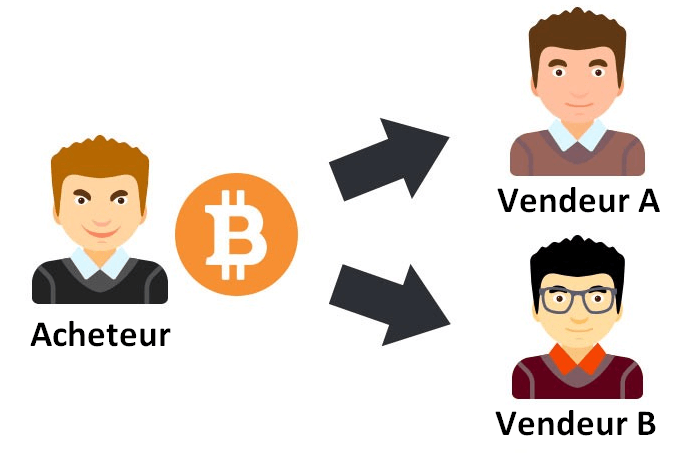
\includegraphics[width=.8\textwidth]{Pictures/double_depense.png}
\end{center}
\end{block}

\begin{block}{Comment le problème est-il résolu ?}
\begin{center}
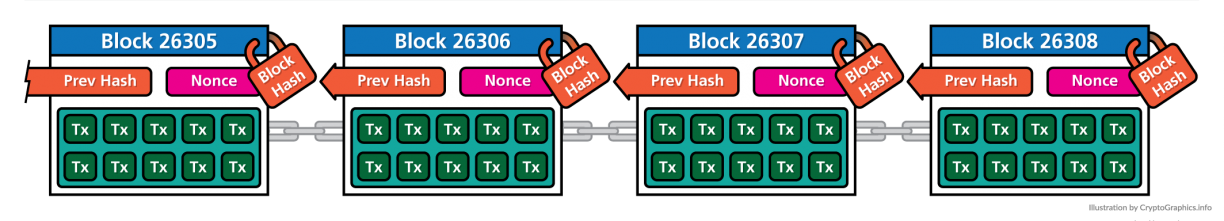
\includegraphics[width=\textwidth]{Pictures/cryptographics/anatomy-of-a-chain-1.png}
\end{center}
\begin{block}<1-4>{avec un journal comptable électronique}
\begin{itemize}
\item <1>organisés en blocks \alert{infalsifiables} : \href{https://andersbrownworth.com/blockchain/hash}{SHA256 HASH}
\item <2>de façon unique : \href{https://andersbrownworth.com/blockchain/block}{block}
\item <3>qui s'\alert{enchainent} les uns aux autres : \href{https://andersbrownworth.com/blockchain/blockchain}{chain}
\item <4>dans un réseau \alert{publique et décentralisé} : \href{https://andersbrownworth.com/blockchain/distributed}{pairs}
\end{itemize}
\end{block}

\begin{block}<5>{Un exemple de block}
\end{block}
\end{block}



\begin{block}{Plus techniquement comment cela fonctionne ?}
\begin{figure}[ht]
   \centering
   \includegraphics<1>[width=.6\textwidth]{Pictures/cryptographics/tx}
   \includegraphics<2>[width=.6\textwidth]{Pictures/cryptographics/block}
   \includegraphics<3>[width=\textwidth]{Pictures/cryptographics/Anatomy-of-a-block2}    
   \includegraphics<4>[width=\textwidth]{Pictures/cryptographics/anatomy-of-a-chain-1}
 \end{figure}

\only<1>{
\href{https://andersbrownworth.com/blockchain/tokens}{Tx}:  ".00012300 BTC pour Binta, signé Amadou"
}
\only<2>{
Les mineurs inclu la \href{https://andersbrownworth.com/blockchain/tokens}{tx dans un bloc} et cherchent un \alert{bon} \emph{nonce}
}
\only<3>{
Le 1\ier{} mineur à trouver un \alert{bon} \emph{nonce}, publie le bloc
\begin{itemize}
\item il contient une récompense (\href{https://andersbrownworth.com/blockchain/coinbase}{coinbase})
\end{itemize}
}
\only<4>{
Les autres mineurs:
\begin{itemize}
\item Vérifient le nonce
\item Ajoutent le nouveau block à la chaine
\item Recommencent la course pour  obtenir une récompense
\end{itemize}

}      
\end{block}


\begin{block}{Et, ça marche depuis 2009 !}
\begin{center}
\includegraphics[width=.7\linewidth]{Pictures/pizza_1millions.jpg}
\end{center}
\begin{itemize}
\item 18/05/2010, \href{https://bitcointalk.org/index.php?topic=137.msg1195}{les Pizza à 10000 BTC de Laslo (bitcointalk.org)}
\end{itemize}
\end{block}
\end{frame}

\begin{frame}[label={sec:org7eec08b}]{Les limites}
\begin{block}{Des problèmes de taille}
\begin{block}{Puissance nécessaire}
\begin{itemize}
\item \href{https://www.blockchain.com/fr/charts/hash-rate}{Hash Rate}  (TeraHash/s, Tera = 1000 milliards)
\end{itemize}
\end{block}
\begin{block}{Vitesse de confirmation}
\begin{itemize}
\item \href{https://www.blockchain.com/explorer/charts/median-confirmation-time}{Attente pour les transactions}
\end{itemize}
\end{block}
\begin{block}{Coût}
\begin{itemize}
\item \href{https://www.blockchain.com/explorer/charts/fees-usd-per-transaction}{Frais de transaction relativement important}
\end{itemize}
\end{block}

\begin{block}{Simplicité}
\end{block}
\begin{block}{Manque d'adaptabilité}
\end{block}
\end{block}

\begin{block}{Coût énergétique}
\begin{center}
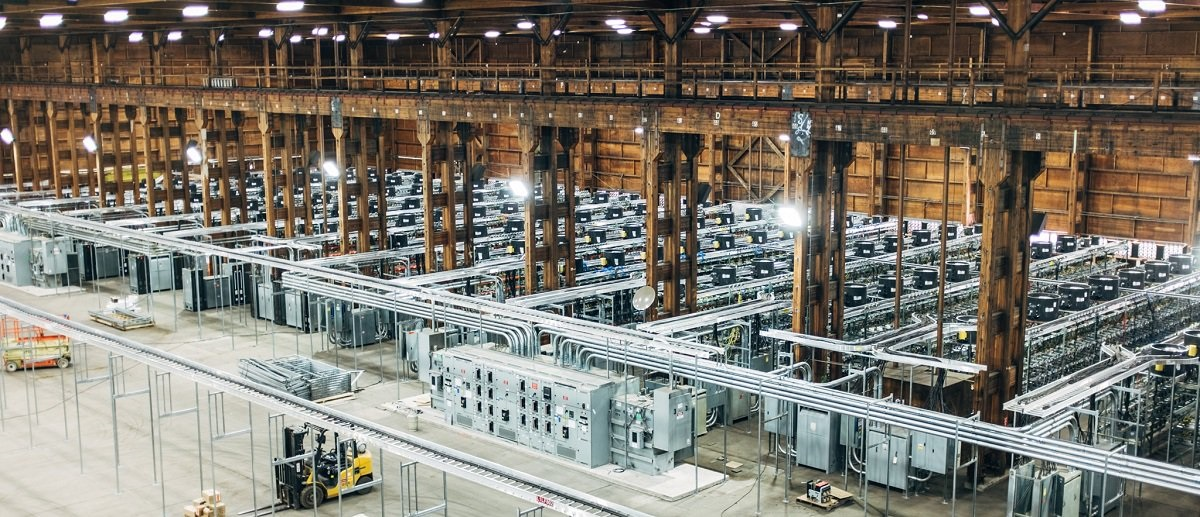
\includegraphics[width=\textwidth]{Pictures/mining-farm-bitcoin.jpg}
\end{center}
\end{block}

\begin{block}{\href{https://www.blockchain.com/charts/pools}{Concentration du hashrate} (janv 2023)}
\begin{center}
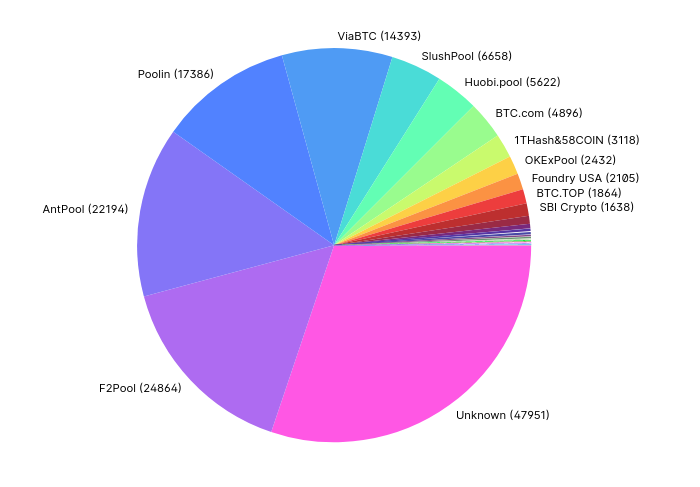
\includegraphics[width=.6\textwidth]{Pictures/hashrate_distrib_jan23.png}
\end{center}
\end{block}

\begin{block}{\href{https://www.blockchain.com/explorer/charts/transactions-per-second}{Vitesse de traitement des transactions}}
\begin{center}
\includegraphics[width=\textwidth]{Pictures/cryptographics/the-scaling-issue.png}
\end{center}
\end{block}
\begin{block}{Jeux d'instructions limités}
\begin{center}
\includegraphics[width=.9\textwidth]{Pictures/automate_simple.jpeg}
\end{center}
\end{block}
\begin{block}{Hard-forks}
\begin{center}
\includegraphics[width=.9\textwidth]{Pictures/cryptographics/blockchain-hard-fork.png}
\end{center}
\end{block}
\end{frame}

\section{Perspectives}
\label{sec:orgf246700}
\begin{frame}[label={sec:org7df0c43}]{Perspectives}
\begin{block}{}
\begin{block}{Naissance d'une techno}
\end{block}
\begin{block}{qui réunie}
\end{block}
\begin{block}{mais qui pourrait être plus efficace}
\end{block}
\end{block}
\end{frame}
\end{document}